%!TEX root = ../thesis.tex  % Comment this line for standalone compilation
%*******************************************************************************
%*********************************** First Chapter Appendix *****************************
%*******************************************************************************

\chapter{Diffusion Models Encode the Intrinsic Dimension of Data Manifolds}

\section{Extended background on diffusion models}
\label{ch3:appendix:background}
\textbf{Setup:}  In \cite{song2020score} score-based  \cite{score_matching} and diffusion-based \cite{diffusion_models, ddpm} generative models have been unified into a single continuous-time score-based framework where the diffusion is driven by a stochastic differential equation.  This framework relies on Anderson's Theorem \cite{anderson1982reverse_time_sde}, which states that under certain Lipschitz conditions on the drift coefficient $f : \mathbb{R}^{n_x} \times \mathbb{R} \xrightarrow{} \mathbb{R}^{n_x}$ and on the diffusion coefficient $G : \mathbb{R}^{n_x} \times \mathbb{R}\xrightarrow{} \mathbb{R}^{n_x} \times \mathbb{R}^{n_x}$ and an integrability condition on the target distribution $p_0(\textbf{x}_0)$ a forward diffusion process governed by the following SDE:
\begin{gather}
\label{ch3:eq:forward_sde}
 d\textbf{x}_t = f(\textbf{x}_t,t)dt+G(\textbf{x}_t,t)d\textbf{w}_t  
\end{gather} 
has a reverse diffusion process governed by the following SDE:
\label{ch3:eq:reverse_sde}
\begin{gather}
    d\textbf{x}_t=[f(\textbf{x}_t,t)-G(\textbf{x}_t,t)G(\textbf{x}_t,t)^T\nabla_{\textbf{x}_t}{\ln{p_t(\textbf{x}_t)}}]dt + G(\textbf{x}_t,t)d\Bar{\textbf{w}_t},
\end{gather}


\noindent where $\Bar{\textbf{w}_t}$ is a standard Wiener process in reverse time. 

The forward diffusion process transforms the \textit{target distribution} $p_0(\textbf{x}_0)$ to a \textit{diffused distribution} $p_T(\textbf{x}_T)$ after diffusion time $T$. By appropriately selecting the drift and the diffusion coefficients of the forward SDE, we can make sure that after sufficiently long time $T$, the diffused distribution $p_T(\textbf{x}_T)$ approximates a simple distribution, such as $\mathcal{N}(\textbf{0},\textbf{I})$. We refer to this simple distribution as the \textit{prior distribution}, denoted by $\pi$. The reverse diffusion process transforms the diffused distribution $p_T(\textbf{x}_T)$ to the data distribution $p_0(\textbf{x}_0)$ and the prior distribution $\pi$ to a distribution $p^{SDE}$. The distribution $p^{SDE}$ is close to $p_0(\textbf{x}_0)$ if the diffused distribution $p_T(\textbf{x}_T)$ is close to the prior distribution $\pi$. We get samples from $p^{SDE}$ by sampling from $\pi$ and simulating the reverse SDE from time $T$ to time $0$.

\textbf{Sampling:} To get samples by simulating the reverse SDE, we need access to the time-dependent \textit{score function} $\nabla_{\textbf{x}_t}{\ln{p_t(\textbf{x}_t)}}$. In practice, we approximate the time-dependent score function with a neural network $s_{\theta}(\textbf{x}_t,t) \approx \nabla_{\textbf{x}_t}{\ln{p_t(\textbf{x}_t)}}$ and simulate the reverse SDE presented in equation \ref{ch3:eq:approximated_reverse_sde} to map the prior distribution $\pi$ to $p^{SDE}_{\theta}$.

\begin{gather}\label{ch3:eq:approximated_reverse_sde}
d\textbf{x}_t=[f(\textbf{x}_t,t)-G(\textbf{x}_t,t)G(\textbf{x}_t,t)^Ts_{\theta}(\textbf{x}_t,t)]dt + G(\textbf{x}_t,t)d\Bar{\textbf{w}_t},
\end{gather}If the prior distribution is close to the diffused distribution and the approximated score function is close to the ground truth score function, the modeled distribution  $p^{SDE}_{\theta}$ is provably close to the target distribution $p_0(\textbf{x}_0)$. This statement is formalised in the language of distributional distances in the work of \cite{song2021maximum}. 

%In diffusion models, the sde in equation \ref{ch3:eq:uniform_sde} describes the forward diffusion for all dimensions in an input tensor:

%\begin{equation}\label{ch3:eq:uniform_sde}
%d\textbf{x}_t=f(\textbf{x}_t,t)dt + g(t)d\Bar{w_t},
%\end{equation}

%We used unbold notation for the random variables to show that this equation describes diffusion in one dimension. 

\textbf{Training:} A neural network $s_\theta(\textbf{x}_t,t)$ can be trained to approximate the score function $\nabla_{\textbf{x}_t}{\ln{p_t(\textbf{x}_t)}}$ by minimizing the weighted score matching objective

\begin{gather}
\begin{aligned}
    \mathcal{L}_{SM}(\theta, \lambda(\cdot)) := 
    \frac{1}{2} \mathbb{E}_{\subalign{&t \sim U(0,T)\\ &\textbf{x}_t \sim p_t(\textbf{x}_t)}} [\lambda(t) \norm{\nabla_{\textbf{x}_t}{\ln{p_t(\textbf{x}_t)}} - s_\theta(\textbf{x}_t,t)}_2^2]
\end{aligned}
\end{gather}
where $\lambda: [0,T] \xrightarrow{} \mathbb{R}_+$ is a positive weighting function.

However, the above quantity cannot be optimized directly since we don't have access to the ground truth score $\nabla_{\textbf{x}_t}{\ln{p_t(\textbf{x}_t)}}$. Therefore in practice, a different objective has to be used \cite{score_matching, vincent2011connection, song2020score}. In \cite{song2020score}, the weighted denoising score-matching objective is used, which is defined as 

\begin{gather}\label{ch3:DSM_for_uniform_diffusion_models}
\begin{aligned}
    \mathcal{L}_{DSM}(\theta, \lambda(\cdot)) := 
    \frac{1}{2} \mathbb{E}_{\subalign{&t \sim U(0,T)\\ &\textbf{x}_0 \sim p_0(\textbf{x}_0) \\ &\textbf{x}_t \sim p_t(\textbf{x}_t | \textbf{x}_0)}} [\lambda(t) \norm{\nabla_{\textbf{x}_t}{\ln{p_t(\textbf{x}_t | \textbf{x}_0)}} - s_\theta(\textbf{x}_t,t)}_2^2]
\end{aligned}
\end{gather}

The difference between DSM and SM is the replacement of the ground truth score which we do not know by the score of the perturbation kernel which we know analytically for many choices of forward SDEs. The choice of the weighted DSM objective is justified because the weighted DSM objective is equal to the SM objective up to a constant that does not depend on the parameters of the model $\theta$. The reader can refer to \cite{vincent2011connection} for the proof. 

\section{Training details}
\label{ch3:sec:hparams}
We trained the score model using the weighted denoising score matching objective \cite{song2020score}, presented in eq. \ref{ch3:DSM_for_uniform_diffusion_models}. We used the likelihood weighting function, i.e. $\lambda(t)=g(t)^2$, where $g(t)$ is the diffusion coefficient of the forward SDE.

\subsection{Euclidean data}
For all of our experiments on Euclidean data, we used a fully connected network with 5 hidden layers and 2048 nodes in each hidden layer to approximate the score function. The input and output dimension is the same as the ambient dimension. For the optimisation of the model, we used the Adam algorithm with a learning rate of $2\mathrm{e}{-5}$ and exponential moving average (EMA) on the weights of the model with a decay rate of $0.9999$. Moreover, we chose the variance exploding SDE \cite{song2020score} as the forward process with $\sigma_{min}=0.01$ and $\sigma_{max}=4$.

\subsection{ Image data}    
For all our of our experiments on image data, we used the DDPM architecture \cite{ho2020denoising} with variance exploding SDE \cite{song2020score} and hyperparameters indicated in Table \ref{ch3:tab:model_params}.

\subsection{Auto-encoder}
The encoder and decoder encoder architectures are based on the DDPM U-Net \cite{ddpm}, which we call half-U nets.

For the encoder we used the downsampling part of the U-Net and removed the upsampling part and the skip connections. The downscaled tensor is flattened and mapped to the latent dimension with an additional linear layer.

For the decoder we start by linearly transforming the latent vector and reshaping it into a tensor of appropriate dimension. Then we used the upsampling part of the DDPM U-Net.

We used the Adam optimizer and EMA rate $0.999$. We used learning rate scheduler reducing the loss on plateau starting form $10^{-4}$ and stopping at $10^{-5}$. We trained the auto-encoder for each latent dimension for 36h on NVIDIA A-100 GPU. At the end we used checkpoints which minimized the validation loss to evaluate the reconstruction error.

All other hyperparameters are included in Table \ref{ch3:tab:model_params}.

\begin{table}[h]
\centering
\begin{tabular}{|l|l|l|}
\hline
\textbf{Hyper-parameter} & \textbf{MNIST} & \textbf{Synthetic Image data} \\
\hline
Number of filters & 128 & 128 \\
\hline
Channel multipliers & (1, 2, 2, 4) & (1, 2, 2, 2) \\
\hline
Dropout & 0.1 & 0.1 \\
\hline
EMA rate & 0.999 & 0.999 \\
\hline
Normalization & GroupNorm & GroupNorm \\
\hline
Nonlinearity & Swish & Swish \\
\hline
Number of residual blocks & 4 & 4 \\
\hline
Attention resolution & 16 & 16 \\
\hline
Convolution size & 3 & 3 \\
\hline
$\sigma_\text{min}$ & $0.009$ & $0.01$ \\
\hline
$\sigma_\text{max}$ & $50$ & $50$  \\
\hline
Learning rate & Scheduler($10^{-4}$, $10^{-5}$) & $2 \cdot 10^{-4}$ \\
\hline
\end{tabular}

\caption{DDPM Model Parameters}
\label{ch3:tab:model_params}
\end{table}

\section{Benchmarking}
\label{ch3:sec:benchmark}
We compared our method against well established approaches to intrinsic dimensionality estimation: the MLE estimator \cite{dim_MLE}, \cite{haro_mle}, Local PCA \cite{fan_local_pca} and Probabilistic PCA \cite{auto_ppca} \cite{ppca}. For MLE estimator and local PCA we used the implementation provided in the R package  \textsc{intrinsicDimension} \cite{R_intrinsic_dim}. The MLE estimator has an important hyperparameter $m$ - the number of nearest neighbour distances that should be used for the dimension estimation. We used values $m=5$ and $20$ since these are extremal values considered in \cite{pope2021intrinsic}. For PPCA we used the \textsc{scikit-learn} implementation \cite{sklearn}. The code for reproducing the benchmarking experiments is included in our codebase.

For the ID-NF method \cite{horvat2022nfid}, we used the official implementation available at \url{https://github.com/chrvt/ID-NF}. For the Euclidean data, we utilized the "vector data" folder, which employs block neural autoregressive flows to learn the normalizing flows, from which the intrinsic dimension is extracted using the ID-NF method. For the synthetic image data and MNIST, we used the "images" folder, which uses rational quadratic splines to train the normalizing flows.

\section{Proofs}
\label{ch3:appendix:proof}
Here we provide full proofs for the statements in Section \ref{ch3:sec:theory}. First, we show that for any point $\textbf{x}$ sufficiently close to the data manifold and sufficiently small $t$ the score $\nabla_\textbf{x} \ln p_t(\textbf{x})$ points directly at the manifold. We demonstrate this by showing that projection of the score in any direction $\boldsymbol{\nu} \perp \textbf{n}$ vanishes in proportion to the projection on $\textbf{n} = \frac{(\pi(\textbf{x}) - \textbf{x})}{\norm{\pi(\textbf{x}) -\textbf{x}}}$ as $t \to 0$. Then Theorem \ref{ch3:thm:score_orthogonal} and Corollary \ref{ch3:cor:score_ratio} will follow easily from this result.

\begin{theorem}
\label{ch3:thm:master_thm}
Suppose that the the support of the data distribution $P_0$ is contained in a compact embedded sub-manifold $\mathcal{M} \subseteq \mathbb{R}^d$ and let $P_t$ be the distribution of samples from $P_0$ diffused for time $t$. Then, under mild assumptions, for any point $\textup{\textbf{x}} \in \mathbb{R}^d$ sufficiently close to $\mathcal{M}$, with orthogonal projection on $\mathcal{M}$, given by $\pi(\textup{\textbf{x}})$. Let $\textup{\textbf{n}}$ be a unit vector pointing from $\textup{\textbf{x}}$ to $\pi(\textup{\textbf{x}})$, then we have that for any unit vector $\boldsymbol{\nu}$ orthogonal to $\textup{\textbf{n}}$: 
\begin{gather*}
    \frac{\boldsymbol{\nu}^T \nabla_\textup{\textbf{x}} \ln p_t(\textup{\textbf{x}})}{\textup{\textbf{n}}^T \nabla_\textup{\textbf{x}} \ln p_t(\textup{\textbf{x}})} \to 0, \text{as } t \to 0.
\end{gather*}
\end{theorem}

\textbf{Assumptions}
\begin{enumerate}
    \item The distribution $P_0$ has a smooth density $p_0$ wrt the volume measure on the manifold.
    \item The density $p_0$ is bounded away from zero on the manifold.
\end{enumerate}

\subsection*{Illustrative simple case}

\begin{figure}
\centering
  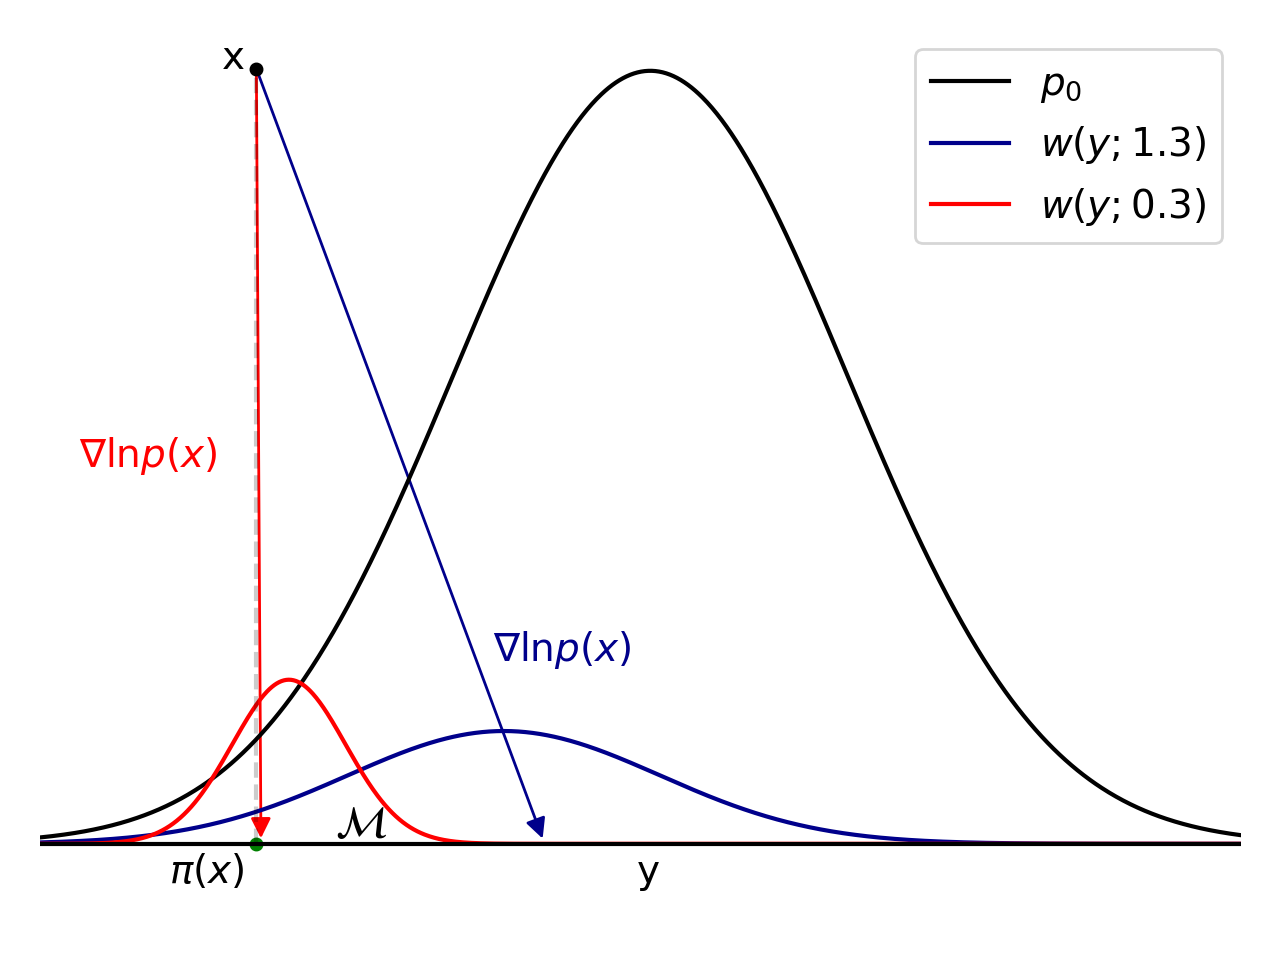
\includegraphics[width=0.7\linewidth]{Chapter3/figures/explanation.png}
  \caption[Caption without FN]{The score is the weighted average of vectors pointing from $\textbf{x}$ to $\textbf{y}$ with weights given by $w(\textbf{y};\sigma_t)$. As $\sigma_t$ decreases weights $w(\textbf{y}; \sigma_t)$ concentrate around $\pi(\textbf{x})$ and the influence of points $\textbf{y}$ away from projection $\pi(\textbf{x})$ becomes insignificant. Therefore, the direction of the score tends to a align with $\pi(\textbf{x})-\textbf{x}$. (Norm of the score vectors on the figure was scaled for better visibility. The direction is preserved.)}
  \label{ch3:fig:example}
\end{figure}

We first present an illustrative proof of a simple case of $\mathcal{M}$ being a linear subspace with $k=1$ and $d=2$. This case gives all of the essential ideas behind the general proof without much of the technicality. For the more interested reader, we then provide a proof of the result for a general manifold, using tools such as the notion of tubular neighbourhoods and some results from Morse theory. 
    
    Without the loss of generality assume that $\mathcal{M} = \{ (x_1,x_2) \in \mathbb{R}^2 : x_2 = 0 \}$ the line given by the $x_1$-axis. Pick a point $\textbf{x} \in \mathbb{R}^2$. The score at point $\textbf{x}$ is given by
\begin{gather*}
    \nabla_\textbf{x} \ln p_t(\textbf{x}) = \frac{1}{\sigma_t^2 p_t(\textbf{x})} \int_\mathcal{M} (\textbf{y}-\textbf{x}) \mathcal{N}(\textbf{y} | \textbf{x}, \sigma^2_t\textbf{I}) p_0(\textbf{y}) d\textbf{y}.
\end{gather*}
Notice that $\mathcal{N}((y_1, y_1) | (x_1, x_2), \sigma^2_t\textbf{I})$\footnote{In component-wise notation $\textbf{y} = (y_1, y_2)$ and $\textbf{x} = (x_1, x_2)$.} is a bivariate normal distribution and its restriction to $\mathcal{M}$ is equal to $\mathcal{N}((y_1, 0) | (x_1, x_2), \sigma^2_t\textbf{I}) = \mathcal{N}(0 | x_2, \sigma^2_t) \mathcal{N}(y_1 | x_1, \sigma^2_t)$. \vspace{0.2cm} Therefore
\begin{gather*}
    \nabla_\textbf{x} \ln p_t(\textbf{x}) = \frac{\mathcal{N}(0 | x_2, \sigma^2_t)}{\sigma_t^2p_t(\textbf{x})} \int_\mathcal{M} (\textbf{y}-\textbf{x})  \mathcal{N}(y_1 | x_1, \sigma^2_t) p_0(\textbf{y}) d\textbf{y}.
\end{gather*}
This means that the score is the weighted average of vectors pointing from $\textbf{x}$ to $\textbf{y}$ over all choices of points $\textbf{y}$ on the manifold, with weights given by $w(\textbf{y};\sigma_t) :=\mathcal{N}(y_1 | x_1, \sigma^2_t) p_0(\textbf{y})$ (see Figure \ref{ch3:fig:example} for visual explanation). For small $\sigma_t$ these weights concentrate around $\pi(\textbf{x})=(x_1,0)$ the projection of $\textbf{x}$ on $\mathcal{M}$, and vanishing far away from it. Consider a ratio of the tangential part to the normal part of the score:
\begin{gather*}
    \frac{\boldsymbol{\nu}^T \nabla_\textbf{x} \ln p_t(\textbf{x})}{\textbf{n}^T \nabla_\textbf{x} \ln p_t(\textbf{x})} = \frac{\int_\mathcal{M} \boldsymbol{\nu}^T(\textbf{y}-\textbf{x})  \mathcal{N}(y_1 | x_1, \sigma^2_t) p_0(\textbf{y}) d\textbf{y}}{\int_\mathcal{M} \textbf{n}^T(\textbf{y}-\textbf{x})  \mathcal{N}(y_1 | x_1, \sigma^2_t) p_0(\textbf{y}) d\textbf{y}} 
    \xrightarrow[\sigma_t \to 0]{}
    \frac{\int_\mathcal{M} \boldsymbol{\nu}^T(\textbf{y}-\textbf{x})  \delta_{x_1}(y_1) p_0(\textbf{y}) d\textbf{y}}{\int_\mathcal{M} \textbf{n}^T(\textbf{y}-\textbf{x})  \delta_{x_1}(y_1) p_0(\textbf{y}) d\textbf{y}} \\
    = \frac{\boldsymbol{\nu}^T ((x_1,0)-\textbf{x})}{\textbf{n}^T ((x_1,0)-\textbf{x})} = \frac{(1,0)^T (0,-x_2)}{(0,1)^T (0,-x_2)} = 0
\end{gather*}
where $\boldsymbol{\nu}$ and $\textbf{n}$ are unit vectors in tangential and normal directions respectively. This implies,
\begin{gather*}
    \text{S}_{\cos} (\textbf{n}, \nabla_\textbf{x} \ln p_t(\textbf{x})) 
    = \frac{\textbf{n}^T  \nabla_\textbf{x} \ln p_t(\textbf{x})}{\norm{ \nabla_\textbf{x} \ln p_t(\textbf{x})}} 
    = \frac{\textbf{n}^T  \nabla_\textbf{x} \ln p_t(\textbf{x})}{\sqrt{(\textbf{n}^T  \nabla_\textbf{x} \ln p_t(\textbf{x}))^2 + (\boldsymbol{\nu}^T  \nabla_\textbf{x} \ln p_t(\textbf{x}))^2}} 
    \\ = \frac{1}{\sqrt{1 + \big( \frac{\boldsymbol{\nu}^T\nabla_\textbf{x} \ln p_t(\textbf{x})}{\textbf{n}^T  \nabla_\textbf{x} \ln p_t(\textbf{x})} \big)^2}} 
    \xrightarrow[t \to 0]{} 1.
\end{gather*}
This establishes the theorem for the simple case. The corollary follows immediately since in the simple case we have $\mathbf{T} = \boldsymbol{\nu}^T$ and $\mathbf{N}=\textbf{n}^T$. \qed

\subsection*{Deriving the formula for the density of $P_t$}
Let $\mathcal{M}$ be a compact $k$-dimensional manifold embedded in $\mathbb{R}^d$.
Let $A \subseteq \mathbb{R}^d$. We define the measure $P_0$ on $\mathbb{R}^d$ as
\begin{gather}
    P_0(A) := \int_{A \cap M} p_0(\textbf{y}) d\textbf{y}
\end{gather}
where $d\textbf{y}$ is the volume form\footnote{Integrating over $A$ using the volume form of $\mathcal{M}$ can be thought of as taking an appropriately re-scaled Lebesgue integral over $A$. That is $P_0(A) = \int_{A \cap \mathcal{M}} p_0(\textbf{y})d\textbf{y} = \int_A \int_{\mathbb{R}^d} \delta (\textbf{s}-\textbf{y})\hat{p}_0(\textbf{s})d\textbf{s} d\textbf{y}$. Where the latter are Lebesgue integrals and $\hat{p}_0(\textbf{s}) = p_0(\textbf{s}) \text{ for } \textbf{s}\in\mathcal{M}$ and zero otherwise.} on $M$ and $p_0$ is a smooth function on $\mathcal{M}$ \footnote{i.e. for any chart $\phi: \mathbb{R}^k \supseteq U \xrightarrow[]{} M$ the composition $p_0 \circ \phi: \mathbb{R}^k \supseteq U \xrightarrow[]{} \mathbb{R}$ is smooth.} such that $\int_\mathcal{M} p_0(\textbf{y}) d\textbf{y} = 1$. Let $f : \mathbb{R}^d \rightarrow \mathbb{R}$ be a $P_0$-measurable function. By approximating $f$ with simple functions (linear combination of indicator functions) we conclude that:
\begin{gather}
\label{ch3:eq:itegrals_on_M}
    \int_A f dP_0 = \int_{A \cap M} f(\textbf{y}) p_0(\textbf{y}) d\textbf{y}
\end{gather}
Consider a measure $P_t$ as a convolution of $P_0$ with a normal distribution on $\mathbb{R}^d$. For any measurable  $A \subseteq \mathbb{R}^d$ we have
\begin{gather*}
    (P_0 \ast  \mathcal{N}_{0, t})(A) := \int_{\mathbb{R}^d}\int_{A-\textbf{y}}d\mathcal{N}_{0, t}(\textbf{x})dP_0(\textbf{y}) = \int_{\mathbb{R}^d}\int_{A-\textbf{y}}\mathcal{N}(\textbf{x} | 0, \sigma^2_t\textbf{I})d\textbf{x} dP_0(\textbf{y}) \\
    =  \int_{\mathbb{R}^d}\int_{A}\mathcal{N}(\textbf{x}-\textbf{y} | 0, \sigma^2_t\textbf{I})d\textbf{x} dP_0(\textbf{y}) =  \int_{\mathbb{R}^d}\int_{A}\mathcal{N}(\textbf{y} | \textbf{x}, \sigma^2_t\textbf{I})d\textbf{x} dP_0(\textbf{y}) \\
    = \int_{A} \int_{\mathbb{R}^d} \mathcal{N}(\textbf{y} | \textbf{x}, \sigma^2_t\textbf{I})dP_0(\textbf{y}) d\textbf{x} \overset{\eqref{ch3:eq:itegrals_on_M}}{=} \int_{A} \int_\mathcal{M} \mathcal{N}(\textbf{y} | \textbf{x}, \sigma^2_t\textbf{I}) p_0(\textbf{y}) d\textbf{y} d\textbf{x}
\end{gather*}
where $d\textbf{y}$ is a volume form on $M$ and $d\textbf{x}$ is a volume form on $\mathbb{R}^d$.
Therefore the measure $P_t$ has a density on $\mathbb{R}^d$ given by:
\begin{gather}
    \label{ch3:convolution}
    p_t(\textbf{x}) = \int_\mathcal{M} \mathcal{N}(\textbf{y} | \textbf{x}, \sigma^2_t\textbf{I}) p_0(\textbf{y}) d\textbf{y}.
\end{gather}
Note the $\mathcal{N}(\textbf{y}|\textbf{x},\sigma^2_t\textbf{I})$ here. Typically one would write this as $\mathcal{N}(\textbf{x}|\textbf{y},\sigma^2_t\textbf{I})$ and think of \eqref{ch3:convolution} as the quantity of probability mass at point $\textbf{x}$ after diffusing for time $t$ with initial distribution $p_0(\textbf{y})$. We instead write it this way as it will be more intuitive to think of \eqref{ch3:convolution} as the average probability mass that intersects the manifold after diffusing from a delta distribution at $\textbf{x}$ (where the average is taken over $p_0(\textbf{y})$). These are of course equivalent as $\mathcal{N}(\textbf{x}|\textbf{y},\sigma^2_t\textbf{I})$ is symmetric is $\textbf{x}$ and $\textbf{y}$.

\subsection*{Tubular Neighbourhoods}
First we need to ensure that the point $\textbf{x}$ has a unique projection on $\mathcal{M}$. This is always true for an $\textbf{x}$ sufficiently close to $\mathcal{M}$. We can formalize this with the notion of \textit{tubular neighbourhood} - a tube around $\mathcal{M}$ such that every point $\textbf{x}$ inside can be uniquely represented as a sum of the point on the manifold and a vector from the normal bundle i.e. $\textbf{x} = \textbf{y} + \textbf{v}$ where $\textbf{y} \in \mathcal{M}$ and $\textbf{v} \in \mathcal{N}_\textbf{y} \mathcal{M}$. Formally:

\begin{definition}
Endpoint Map\\
The endpoint map $Y: \mathcal{NM} \xrightarrow[]{} \mathbb{R}^d$ is defined by $Y(\textbf{y}, \textbf{v}) = \textbf{y} + \textbf{v}$ for $\textbf{y} \in \mathcal{M}$ and $\textbf{v} \in \mathcal{N}_\textbf{y} \mathcal{M}$. 
\end{definition}

\begin{definition}
Tubular Neighbourhood\\
A (uniform) tubular neighbourhood of $\mathcal{M}$ is a neighbourhood $U_R$ of $\mathcal{M}$ in $\mathbb{R}^d$ that is a diffeomorphic image under the endpoint map of an open subset $V_R \subseteq \mathcal{NM}$ of the form:
\begin{gather*}
    V_R = \{ (\textbf{y},\textbf{v}) \in \mathcal{NM}: \norm{\textbf{v}}_2 < R \} 
\end{gather*}
\end{definition}
Since $Y$ restricted to $V_R$ is a diffeomorphism\footnote{so in particular it is a bijection}, it follows  that every point $\textbf{x} = (\textbf{y},\textbf{v})$ in the tubular neighbourhood has a unique orthogonal projection on $\mathcal{M}$ given by $\textbf{y}$. We will denote this projection as $\pi(\textbf{x})$.

Conveniently, it turns out that every  compact embedded submanifold of $\mathbb{R}^d$ has a tubular neighborhood.

\begin{theorem}
Tubular Neighborhood Theorem [Theorem 5.25]\cite{lee2019_riemman} \\  
Every  compact  embedded submanifold of $\mathbb{R}^d$ has a uniform tubular neighborhood.
\end{theorem}

\subsection*{Preliminary lemmas and  Morse theory}
In this section we will establish that for every $\textbf{x}$ in the tubular neighbourhood of $\mathcal{M}$ there exists an open neighbourhood $E$ of $\pi(\textbf{x})$ such that:
\begin{enumerate}
    \item $\textbf{n}^T(\textbf{y}-\textbf{x}) > \norm{\pi(\textbf{x}) - \textbf{x}}_2 - \varepsilon $ on $E$ .
    \item $|\boldsymbol{\nu}^T(\textbf{y}-\textbf{x})| < \varepsilon$ on $E$.
    \item %For every $\textbf{y}$ in $E$ we have $\norm{\textbf{x} - \textbf{y}} < M  := \min_{y \in \mathcal{M} \setminus E} \norm{\textbf{x} - \textbf{y}}_2$. Which implies
    The mass of a Gaussian centred at $\textbf{x}$ is concentrated in $E$,
    $$ \frac{\int_{\mathcal{M} \setminus E}\mathcal{N}(\textbf{y} | \textbf{x}, \sigma^2_t\textbf{I}) d\textbf{y}}{ \int_E \mathcal{N}(\textbf{y} | \textbf{x}, \sigma^2_t\textbf{I}) d\textbf{y}} \to 0 \text{ as } t \to 0. $$
\end{enumerate}

We begin by defining an $E$ which satisfies the first two conditions.
\begin{lemma}
\label{ch3:lemma:small_projection}
Choose $E$ contained in a ball of radius $0 < \varepsilon < \norm{\textup{\textbf{x}} - \pi(\textup{\textbf{x}})}$ around $\pi(\textup{\textbf{x}})$. Let $\textup{\textbf{y}} \in E$, and let $ \textup{\textbf{v}}_\varepsilon := \textup{\textbf{y}} - \pi(\textup{\textbf{x}}) $. Then 
    \begin{enumerate}
        \item $\textup{\textbf{n}}^T(\textup{\textbf{y}}-\textup{\textbf{x}}) > \norm{\pi(\textup{\textbf{x}}) - \textup{\textbf{x}}}_2 - \varepsilon $ on $E$ .
        \item $|\boldsymbol{\nu}^T(\textup{\textbf{y}}-\textup{\textbf{x}})| < \varepsilon$ on $E$.
    \end{enumerate}
\end{lemma}
\begin{proof}
By direct computation
\begin{align*}
   \textbf{n}^T(\textbf{y}-\textbf{x}) &= \textbf{n}^T( (\textbf{x} - \pi(\textbf{x})) + \textbf{v}_\varepsilon)\\
   &= \textbf{n}^T(\textbf{x} - \pi(\textbf{x})) + \textbf{n}^T\textbf{v}_\varepsilon \\
   &= \norm{\textbf{x} - \pi(\textbf{x})}_2 + \textbf{n}^T\textbf{v}_\varepsilon\\
   &\geq  \norm{\textbf{x} - \pi(\textbf{x})} - \norm{\textbf{v}_\varepsilon}_2.
\end{align*}   
We have that $\norm{\textbf{v}_\varepsilon} < \varepsilon$, hence for all $\textbf{y}$ in $E$ we have that $ \textbf{n}^T(\textbf{y}-\textbf{x}) \geq \norm{\textbf{x} - \pi(\textbf{x})} - \varepsilon > 0 $. For the second inequality \begin{align*}
    | \boldsymbol{\nu}^T(\textbf{y}-\textbf{x}) | &\leq | \boldsymbol{\nu}^T( (\textbf{x} - \pi(\textbf{x}))| + |\boldsymbol{\nu}^T\textbf{v}_\varepsilon|  \\
    &\leq  \norm{\textbf{v}_\varepsilon}_2 \\ 
    &\leq \varepsilon.
\end{align*}
\end{proof}


Now to find $E$ which also satisfies the last condition we proceed by recalling some elementary definitions and results of Morse theory.

\begin{theorem}
Morse lemma [Corollary 1.17]\cite{nicolaescu2011morse_theory} \\
If $\textup{\textbf{y}}_0$ is a non-degenerate critical point of index $\gamma$ of a smooth function $f : \mathcal{M} \xrightarrow[]{} \mathbb{R}$, then there exist a chart $\phi = (\phi_i)_{i=1}^k$  in a neighbourhood $U$ of $\textup{\textbf{y}}_0$ such that $\phi(\textbf{y}_0) = 0$, and in this chart we have the equality:
$$ f(\textup{\textbf{y}}) = f(\textup{\textbf{y}}_0) - \sum_{i=1}^\gamma \phi_i(\textup{\textbf{y}})^2 + \sum_{i=\gamma + 1}^k \phi_i(\textup{\textbf{y}})^2 $$
\end{theorem}

Let $f_\textup{\textbf{x}}(\textbf{y}): \mathcal{M} \xrightarrow[]{} \mathbb{R}$  denote the squared distance function from $\textbf{x}$ given by $f_\textup{\textbf{x}}(\textbf{y}) = \norm{\textbf{x} - \textbf{y}}_2^2$.
We will establish that if $\textbf{x}$ is in a tubular neighbourhood, then its projection $\pi(\textbf{x})$ is a non-degenerate critical point of $f_\textup{\textbf{x}}$ of index zero.


\begin{definition}
Focal point \\
A point $\textbf{x} =Y(\textbf{y}, \textbf{v})$ in the image of the endpoint map $Y$, is called a non-focal point of $\mathcal{M}$ with respect to $\textbf{y}$ if $dY(\textbf{y},\textbf{v})$ is an isomorphism. Otherwise it is called a focal point.
\end{definition}

\begin{theorem}
Critical points and focal points \cite{palais1988critical}
 \\
Let $\mathcal{M}$ be an embedded submanifold of $\mathbb{R}^d$, $\textup{\textbf{y}} \in M$, $\textup{\textbf{v}} \in \mathcal{N}_\textup{\textbf{y}}\mathcal{M}$, and $\textup{\textbf{x}} = Y (\textup{\textbf{y}},\textup{\textbf{v}}) = \textup{\textbf{y}} + \textup{\textbf{v}}$. Then
\begin{enumerate}
    \item $\textup{\textbf{y}}$ is a critical point of $f_\textup{\textbf{x}}$.
    \item $\textup{\textbf{y}}$ is a non-degenerate critical point of $f_\textup{\textbf{x}}$ if and only if $\textup{\textbf{x}}$ is a non-focal point.
    \item Index of $f_a$ at $\textbf{y}$ is equal to the number of focal points of $\mathcal{M}$ with respect to $\textup{\textbf{y}}$ on the line segment joining $\textup{\textbf{y}}$ to $\textup{\textbf{x}}$.
\end{enumerate}
\end{theorem}
Because the restriction of the endpoint map $Y$ to the tubular neighbourhood is a diffeomorphism, the differential $dY$ is an isomorphism for every point in the tubular neighbourhood. Therefore there are no focal points of $\mathcal{M}$ in the tubular neighbourhood. Hence, it follows directly from the above theorem, that if $\textbf{x}$ is in the tubular neighbourhood, then the projection $\pi(\textbf{x})$ is a non-degenerate critical point of $f_\textup{\textbf{x}}$ of index zero. Now we are ready to prove the following lemma.

\begin{lemma}
\label{ch3:lemma:gaussian_concentration}
    There exists a connected open neighbourhood $E$ of $\pi(\textup{\textbf{x}})$ satisfying conditions of lemma \ref{ch3:lemma:small_projection} and such that, 
    \begin{gather}
        \frac{\int_{\mathcal{M} \setminus E}\mathcal{N}(\textup{\textbf{y}} | \textup{\textbf{x}}, \sigma^2_t\textup{\textbf{I}}) d\textup{\textbf{y}}}{ \int_E \mathcal{N}(\textup{\textbf{y}} | \textup{\textbf{x}}, \sigma^2_t\textup{\textbf{I}}) d\textup{\textbf{y}}} \to 0 \text{ as } t \to 0. 
    \end{gather}
\end{lemma}
\begin{proof}
Fix $\varepsilon > 0$. Then conditions of lemma \ref{ch3:lemma:small_projection} are satisfied inside $B(\pi(\textbf{x}), \varepsilon)$. We have demonstrated that $\pi(\textbf{x})$ fulfills the criteria stipulated by the Morse lemma. Consequently, we can pick $\tilde{U}$ as the neighborhood and $\phi$ as the coordinate system that the Morse lemma provides. Now let $U = \tilde{U} \cap B(\pi(\textbf{x}), \varepsilon)$. Since $\mathcal{M}$ is compact and $U$ is open, there exists $m = \min_{\mathcal{M} \setminus U} f_\textup{\textbf{x}}(\textbf{y})$ and by uniqueness of projection $f_\textup{\textbf{x}}(\pi(\textbf{x})) < m$. 
Let $r= \sqrt{m - (f_\textup{\textbf{x}}(\pi(\textbf{x}))) / 2}$ and let $E = \phi^{-1}(B(0, r))$. For all $\textbf{y} \in E$ we have:
$$f_\textup{\textbf{x}}(\textbf{y}) = f_\textup{\textbf{x}}(\pi(\textbf{x})) + \norm{\phi(\textbf{y})}^2 <   f_\textup{\textbf{x}}(\pi(\textbf{x})) + r^2 < m.$$ 
Notice that for every $\textbf{y} \in U \setminus E$ we have $f_\textup{\textbf{x}}(\textbf{y}) \geq f_\textup{\textbf{x}}(\pi(\textbf{x})) + r^2$. Therefore we have established that
\begin{gather}
\label{ch3:eq:less}
   \forall_{\textbf{y} \in E} \forall_{\tilde{\textbf{y}} \in \mathcal{M} \setminus E } f_\textup{\textbf{x}}(\textbf{y}) < f_\textup{\textbf{x}}(\tilde{\textbf{y}}). 
\end{gather}
Computing directly, we have   
\begin{gather}
\label{ch3:eq:normals2}
    \frac{\int_{\mathcal{M} \setminus E}\mathcal{N}(\textbf{y} | \textbf{x}, \sigma^2_t\textbf{I}) d\textbf{y}}{ \int_E \mathcal{N}(\textbf{y} | \textbf{x}, \sigma^2_t\textbf{I}) d\textbf{y}}
    = \frac{\int_{\mathcal{M} \setminus E} \exp\{{-f_\textup{\textbf{x}}(\textbf{y})/2\sigma_t^2}\} d\textbf{y}}{ \int_E \exp \{{-f_\textup{\textbf{x}}(\textbf{y})/2\sigma_t^2} \}d\textbf{y}} 
\end{gather}
By the mean value theorem there exists $\textbf{y}^*\in E$ and $\tilde{\textbf{y}}^*\in \mathcal{M} \setminus E$ such that 
\begin{align*}
    \int_E \exp \{{-f_\textup{\textbf{x}}(\textbf{y})/2\sigma_t^2} \}d\textbf{y} &= \text{Vol}(E)\exp\{-f_\textup{\textbf{x}}(\textbf{y}^*)/2\sigma_t^2 \} \\
    \int_{\mathcal{M} \setminus E} \exp \{{-f_\textup{\textbf{x}}(\textbf{y})/2\sigma_t^2} \}d\textbf{y} &= \text{Vol}(\mathcal{M} \setminus E)\exp\{-f_\textup{\textbf{x}}(\tilde{\textbf{y}}^*)/2\sigma_t^2 \}
\end{align*}
We can use this to evaluate (\ref{ch3:eq:normals2}) to give,
\begin{align*}
    \frac{\int_{\mathcal{M} \setminus E}\mathcal{N}(\textbf{y} | \textbf{x}, \sigma^2_t\textbf{I}) d\textbf{y}}{ \int_E \mathcal{N}(\textbf{y} | \textbf{x}, \sigma^2_t\textbf{I}) d\textbf{y}} 
    &= \frac{\text{Vol}(\mathcal{M} \setminus E) \exp \left\{-f_\textup{\textbf{x}}(\tilde{\textbf{y}}^*) / 2 \sigma_t^2\right\}}{\text{Vol}(E) \exp \left\{-f_\textup{\textbf{x}}(\textbf{y}^*) / 2 \sigma_t^2 \right\}} \\
    &= \frac{\text{Vol}(\mathcal{M} \setminus E)}{\text{Vol}(E)} \exp \left\{- \frac{f_\textup{\textbf{x}}(\tilde{\textbf{y}}^*) - f_\textup{\textbf{x}}(\textbf{y}^*)}{2 \sigma_t^2}\right\}
\end{align*}

Since by (\ref{ch3:eq:less}) $f_\textup{\textbf{x}}(\tilde{\textbf{y}}^*) - f_\textup{\textbf{x}}(\textbf{y}^*) > 0$  the above goes to zero as $\sigma_t$ goes to zero. Moreover, since $E \subseteq U \subseteq B(\pi(\textbf{x}), \varepsilon)$, the conditions of lemma \ref{ch3:lemma:small_projection} are also satisfied.
\end{proof}

\subsection*{Proof of Theorem \ref{ch3:thm:master_thm}}

Fix $\varepsilon > 0$. Assume that $\textbf{x}$ is in a tubular neighbourhood of $\mathcal{M}$, so that the projection $\pi(\textbf{x})$ exists. To simplify the expressions that appear multiple times, we define the following functions:
\[
g(\textbf{y}, \textbf{x}, t) = \boldsymbol{\nu}^T (\textbf{y}-\textbf{x}) \mathcal{N}(\textbf{y} | \textbf{x}, \sigma^2_t \textbf{I}) p_0(\textbf{y}).
\]

\[
h(\textbf{y}, \textbf{x}, t) = \textbf{n}^T (\textbf{y}-\textbf{x}) \mathcal{N}(\textbf{y} | \textbf{x}, \sigma^2_t \textbf{I}) p_0(\textbf{y}),
\]

Then, we have

\begin{gather}
\label{ch3:eq:begin_proof}
    \frac{\boldsymbol{\nu}^T \nabla_\textbf{x} \ln p_t(\textbf{x})}{\textbf{n}^T \nabla_\textbf{x} \ln p_t(\textbf{x})}   = \frac{\boldsymbol{\nu}^T \nabla_\textbf{x}  p_t(\textbf{x})}{\textbf{n}^T \nabla_\textbf{x}  p_t(\textbf{x})} = \frac{\int_\mathcal{M} g(\textbf{y}, \textbf{x}, t)\, d\textbf{y}}{\int_\mathcal{M} h(\textbf{y}, \textbf{x}, t)\, d\textbf{y}}.
\end{gather}

Split $\mathcal{M}$ into two parts: $E$ and $\mathcal{M} \setminus E$, where $E=B(\textbf{x}, r) \cap \mathcal{M}$ is an open neighbourhood of $\pi(\textbf{x})$ in $\mathcal{M}$ satisfying the conditions of Lemma \ref{ch3:lemma:gaussian_concentration} and Lemma \ref{ch3:lemma:small_projection} for a chosen $\varepsilon > 0$. Then, we have that \eqref{ch3:eq:begin_proof} is equal to

\begin{gather}
    \label{ch3:eq:two_terms}
       \frac{\int_{E} g(\textbf{y}, \textbf{x}, t)\, d\textbf{y}}{\int_\mathcal{M} h(\textbf{y}, \textbf{x}, t)\, d\textbf{y}} + \frac{\int_{\mathcal{M} \setminus E} g(\textbf{y}, \textbf{x}, t)\, d\textbf{y}}{\int_\mathcal{M} h(\textbf{y}, \textbf{x}, t)\, d\textbf{y}}.
\end{gather}

\noindent We begin by bounding the first term:
\begin{align*}
    \frac{\int_{E} g(\textbf{y}, \textbf{x}, t)\, d\textbf{y}}{\int_\mathcal{M} h(\textbf{y}, \textbf{x}, t)\, d\textbf{y}} & = \frac{\int_{E} g(\textbf{y}, \textbf{x}, t)\, d\textbf{y}}{\int_E h(\textbf{y}, \textbf{x}, t)\, d\textbf{y} + \int_{\mathcal{M} \setminus E} h(\textbf{y}, \textbf{x}, t)\, d\textbf{y}} \\
    & = \frac{ \dfrac{\int_{E} g(\textbf{y}, \textbf{x}, t)\, d\textbf{y}}{\int_{E} h(\textbf{y}, \textbf{x}, t)\, d\textbf{y}}  }{1 + \dfrac{ \int_{\mathcal{M} \setminus E} h(\textbf{y}, \textbf{x}, t)\, d\textbf{y}}{\int_{E} h(\textbf{y}, \textbf{x}, t)\, d\textbf{y}}} \\
    & =: \frac{A_t}{1+B_t}.
\end{align*}

For $A_t$, we have
\begin{gather*}
    |A_t| = \bigg| \frac{\int_{E} g(\textbf{y}, \textbf{x}, t)\, d\textbf{y}}{\int_{E} h(\textbf{y}, \textbf{x}, t)\, d\textbf{y}} \bigg|. 
\end{gather*}
Using the fact that $\textbf{n}^T (\textbf{y}-\textbf{x})$ is positive and bounded away from zero and applying the triangle inequality, we obtain
\begin{align*}
    |A_t| &\leq \frac{\int_{E} |\boldsymbol{\nu}^T (\textbf{y}-\textbf{x})| \mathcal{N}(\textbf{y} | \textbf{x}, \sigma^2_t \textbf{I}) p_0(\textbf{y})\, d\textbf{y}}{\int_{E} h(\textbf{y}, \textbf{x}, t)\, d\textbf{y}} \\
        &\leq \frac{ \varepsilon\, p_\text{max} \int_{E} \mathcal{N}(\textbf{y} | \textbf{x}, \sigma^2_t \textbf{I})\, d\textbf{y}}{ (\|\pi(\textbf{x}) - \textbf{x}\| - \varepsilon )\, p_\text{min} \int_{E} \mathcal{N}(\textbf{y} | \textbf{x}, \sigma^2_t \textbf{I})\, d\textbf{y}} \\
    &= \frac{p_\text{max}}{p_\text{min}} \frac{ \varepsilon}{\|\pi(\textbf{x}) - \textbf{x}\| - \varepsilon},
\end{align*}
where in the second inequality we used that $0 < p_\text{min} < p_0(\textbf{y}) < p_\text{max}$, $|\boldsymbol{\nu}^T(\textbf{y}-\textbf{x})| < \varepsilon$, and $\textbf{n}^T(\textbf{y}-\textbf{x}) > \|\pi(\textbf{x}) - \textbf{x}\| - \varepsilon$ on $E$.

Since $\varepsilon$ was arbitrary, this term can be made arbitrarily small.

Now we move to $B_t$. Let $D = \max_{\textbf{y} \in \mathcal{M}} \|\textbf{x} - \textbf{y}\|$. By the triangle and Cauchy-Schwarz inequalities, we have
\begin{align*}
    |B_t| &\leq \frac{ \int_{\mathcal{M} \setminus E} |\textbf{n}^T (\textbf{y}-\textbf{x})| \mathcal{N}(\textbf{y} | \textbf{x}, \sigma^2_t \textbf{I}) p_0(\textbf{y})\, d\textbf{y}}{\int_{E} h(\textbf{y}, \textbf{x}, t)\, d\textbf{y}} \\
    &\leq \frac{ p_\text{max} D}{ p_\text{min} (\|\pi(\textbf{x}) - \textbf{x}\| - \varepsilon)} \frac{\int_{\mathcal{M} \setminus E}  \mathcal{N}(\textbf{y} | \textbf{x}, \sigma^2_t \textbf{I})\, d\textbf{y}}{\int_{E} \mathcal{N}(\textbf{y} | \textbf{x}, \sigma^2_t \textbf{I})\, d\textbf{y}},
\end{align*}
which goes to zero as $t$ goes to zero.

Finally, we move to the second term in (\ref{ch3:eq:two_terms}). We start with the same steps as with the first term:
\begin{gather*}
    \frac{\int_{\mathcal{M} \setminus E} g(\textbf{y}, \textbf{x}, t)\, d\textbf{y}}{\int_\mathcal{M} h(\textbf{y}, \textbf{x}, t)\, d\textbf{y}}
    = \frac{ \dfrac{\int_{\mathcal{M} \setminus E} g(\textbf{y}, \textbf{x}, t)\, d\textbf{y}}{\int_{E} h(\textbf{y}, \textbf{x}, t)\, d\textbf{y}}  }{1 + \dfrac{ \int_{\mathcal{M} \setminus E} h(\textbf{y}, \textbf{x}, t)\, d\textbf{y}}{\int_{E} h(\textbf{y}, \textbf{x}, t)\, d\textbf{y}} } 
    =: \frac{C_t}{1 + B_t},
\end{gather*}
so we only need to examine $C_t$. By the triangle and Cauchy-Schwarz inequalities again, we have
\begin{align*}
    |C_t| &\leq \frac{\int_{\mathcal{M} \setminus E} |\boldsymbol{\nu}^T (\textbf{y}-\textbf{x})| \mathcal{N}(\textbf{y} | \textbf{x}, \sigma^2_t \textbf{I}) p_0(\textbf{y})\, d\textbf{y}}{\int_{E} h(\textbf{y}, \textbf{x}, t)\, d\textbf{y}} \\
    &\leq \frac{ p_\text{max} D}{ p_\text{min} (\|\pi(\textbf{x}) - \textbf{x}\| - \varepsilon)} \frac{\int_{\mathcal{M} \setminus E}  \mathcal{N}(\textbf{y} | \textbf{x}, \sigma^2_t \textbf{I})\, d\textbf{y}}{\int_{E} \mathcal{N}(\textbf{y} | \textbf{x}, \sigma^2_t \textbf{I})\, d\textbf{y}},
\end{align*}
which goes to zero as $t$ goes to zero.

Putting it all together:
\begin{align*}
    \frac{|\boldsymbol{\nu}^T \nabla_\textbf{x} \ln p_t(\textbf{x})|}{|\textbf{n}^T \nabla_\textbf{x} \ln p_t(\textbf{x})|} 
    &= \frac{|A_t + C_t|}{|1 + B_t|} \\
      &\leq \frac{1}{|1 + B_t|} \left(  \frac{p_\text{max}}{p_\text{min}} \frac{ \varepsilon}{\|\pi(\textbf{x}) - \textbf{x}\| - \varepsilon } + |C_t| \right) \\
      &\xrightarrow[t \to 0]{} \frac{p_\text{max}}{p_\text{min}} \frac{ \varepsilon}{\|\pi(\textbf{x}) - \textbf{x}\| - \varepsilon }.
\end{align*}
Since $\varepsilon$ can be chosen arbitrarily small, this finishes the proof. \qed

    \subsection*{Proof of Theorem \ref{ch3:thm:score_orthogonal}}
    Beginning with $\textbf{n}$ and extending to an orthonormal basis ($\textbf{n}$, $\boldsymbol{\nu}_1$, ... , $\boldsymbol{\nu}_{d-1}$) of $\mathbb{R}^d$, we have
    \begin{gather*}
        \text{S}_{\cos} (\textbf{n}, \nabla_\textbf{x} \ln p_t(\textbf{x})) = \frac{\textbf{n}^T\nabla_\textbf{x} \ln p_t(\textbf{x})}{\norm{\nabla_\textbf{x} \ln p_t(\textbf{x})}} 
        = \frac{\textbf{n}^T(\nabla_\textbf{x} \ln p_t(\textbf{x}))}{\sqrt{ (\textbf{n}^T\nabla_\textbf{x} \ln p_t(\textbf{x}))^2 + \sum_{i=1}^{d-1}(\boldsymbol{\nu}_i^T\nabla_\textbf{x} \ln p_t(\textbf{x}))^2 }} \\
        = \frac{1}{\sqrt{ 1 + \sum_{i=1}^{d-1}\big( \frac{\boldsymbol{\nu}_i^T\nabla_\textbf{x} \ln p_t(\textbf{x})}{\textbf{n}^T\nabla_\textbf{x} \ln p_t(\textbf{x})} \big)^2 }} 
         \xrightarrow[t \to 0]{} 1,
    \end{gather*}
    where in taking the limit we applied the Theorem \ref{ch3:thm:master_thm}. \qed
    
    \subsection*{Proof of Corollary \ref{ch3:cor:score_ratio}}
    Let $(\boldsymbol{\tau}_1, ..., \boldsymbol{\tau}_k)$ be an orthonormal basis of the tangent space $T_{\pi(\textbf{x})}\mathcal{M}$ and extend $\textbf{n}$ to an orthonormal basis $(\textbf{n}, \boldsymbol{\eta}_1, ..., \boldsymbol{\eta}_{d-k-1})$ of the normal space $\mathcal{N}_{\pi(\textbf{x})}\mathcal{M}$.
    Then the projection of the score on the tangent space is given by $\mathbf{T} \nabla_\textbf{x} \ln p_t(\textbf{x}) = \sum_{i=1}^k (\boldsymbol{\tau}_i^T\nabla_\textbf{x} \ln p_t(\textbf{x})) \boldsymbol{\tau}_i$, while the projection on the normal space is  $\mathbf{N} \nabla_\textbf{x} \ln p_t(\textbf{x}) = (\textbf{n}^T\nabla_\textbf{x} \ln p_t(\textbf{x})) \textbf{n} +  \sum_{i=1}^{d-k-1} (\boldsymbol{\eta}_i^T\nabla_\textbf{x} \ln p_t(\textbf{x})) \boldsymbol{\eta}_i$. Therefore
    \begin{gather*}
        \frac{\norm{\mathbf{T} \nabla_\textbf{x} \ln p_t(\textbf{x}) }}{\norm{\mathbf{N} \nabla_\textbf{x} \ln p_t(\textbf{x}) }} = \sqrt{\frac{\sum_{i=1}^k (\boldsymbol{\tau}_i^T\nabla_\textbf{x} \ln p_t(\textbf{x}))^2 }{ (\textbf{n}^T\nabla_\textbf{x} \ln p_t(\textbf{x}))^2 +  \sum_{i=1}^{d-k-1} (\boldsymbol{\eta}_i^T\nabla_\textbf{x} \ln p_t(\textbf{x}))^2 }}
        \\ = \sqrt{\frac{\sum_{i=1}^k \big( \frac{\boldsymbol{\tau}_i^T\nabla_\textbf{x} \ln p_t(\textbf{x})}{\textbf{n}^T\nabla_\textbf{x} \ln p_t(\textbf{x})} \big)^2 }{ 1 +  \sum_{i=1}^{d-k-1} \big( \frac{\boldsymbol{\eta}_i^T\nabla_\textbf{x} \ln p_t(\textbf{x})}{\textbf{n}^T\nabla_\textbf{x} \ln p_t(\textbf{x})} \big)^2 }}
        \xrightarrow[t \to 0]{} 0
    \end{gather*}
    where in taking the limit we applied the Theorem \ref{ch3:thm:master_thm}. \qed

    \section{Details on the design of synthetic image manifolds}\label{ch3:Appendix:_design_of_synthetic_image_manifolds}

    \textbf{Squares image manifold:} We generated the \textit{k-squares dataset} whose intrinsic dimension is controllable and is set to $k$. This dataset comprises 32 × 32 pixel images of squares, generated by first establishing fixed square center locations and side lengths (either 3 or 5 units) across all datapoints. For each square in a given image, we uniformly sampled a brightness value from the unit interval for all pixels within the square's boundary, summing values at points of intersection. The dimension of this manifold is equal to the number of squares $k$ and the ambient space dimension is $32\times32=1024$. We provide samples in Figure \ref{ch3:fig:squares}.
    
    \textbf{Gaussian blobs image manifold:} The Squares image manifold is contained in a low dimensional linear subspace which allowed PPCA to estimate the dimension very well. For this reason, we constructed a synthetic image manifold of known dimension, which cannot be contained in any low dimensional linear subspace.  We replace the squares by Gaussian blobs (i.e. brightness of pixels withing each blob is proportional to a Gaussian pdf). We randomly pick the centers of the Gaussian blobs which remain fixed for all datapoints. For each datapoint, we sample the standard deviation of each Gaussian blob uniformly from the interval $[1,5]$. The dimension of this manifold is equal to the number of Gaussian blobs. We provide samples in Figure \ref{ch3:fig:gaussian-blobs}.

    \begin{figure}[h]
        \centering
        \begin{minipage}{.3\textwidth}
            \centering
            
\includegraphics[width=.75\columnwidth]{chapter3/figures/image_manifolds/squares/10.png}
        \end{minipage}
        \begin{minipage}{.3\textwidth}
            \centering
            
\includegraphics[width=.75\columnwidth]{chapter3/figures/image_manifolds/squares/20.png}
        \end{minipage}
        \begin{minipage}{.3\textwidth}
            \centering
            \includegraphics[width=.75\columnwidth]{chapter3/figures/image_manifolds/squares/100.png}
        \end{minipage} 
        \caption{Nine samples from Squares image manifolds of dimensions 10, 20 and 100 (from left to right).}
        \label{ch3:fig:squares}
        \vspace{10pt}
       \begin{minipage}{.3\textwidth}
            \centering
            
\includegraphics[width=.75\columnwidth]{chapter3/figures/image_manifolds/blobs/10.png}
        \end{minipage}
        \begin{minipage}{.3\textwidth}
            \centering
            
\includegraphics[width=.75\columnwidth]{chapter3/figures/image_manifolds/blobs/20.png}
        \end{minipage}
        \begin{minipage}{.3\textwidth}
            \centering
            \includegraphics[width=.75\columnwidth]{chapter3/figures/image_manifolds/blobs/100.png}
        \end{minipage} 
        \caption{Nine samples from Gaussian blob image manifolds of dimensions 10, 20 and 100 (from left to right).}
        \label{ch3:fig:gaussian-blobs}     
   \end{figure}

   \section{Additional Experimental Results}
   \label{ch3:appendix:additional_experimental_results}
   
   \subsection{Euclidean Data}
   \label{ch3:appendix:additional_euclidean}
   
   \begin{figure}[H]
   \begin{minipage}[t]{.45\textwidth}
       \centering
       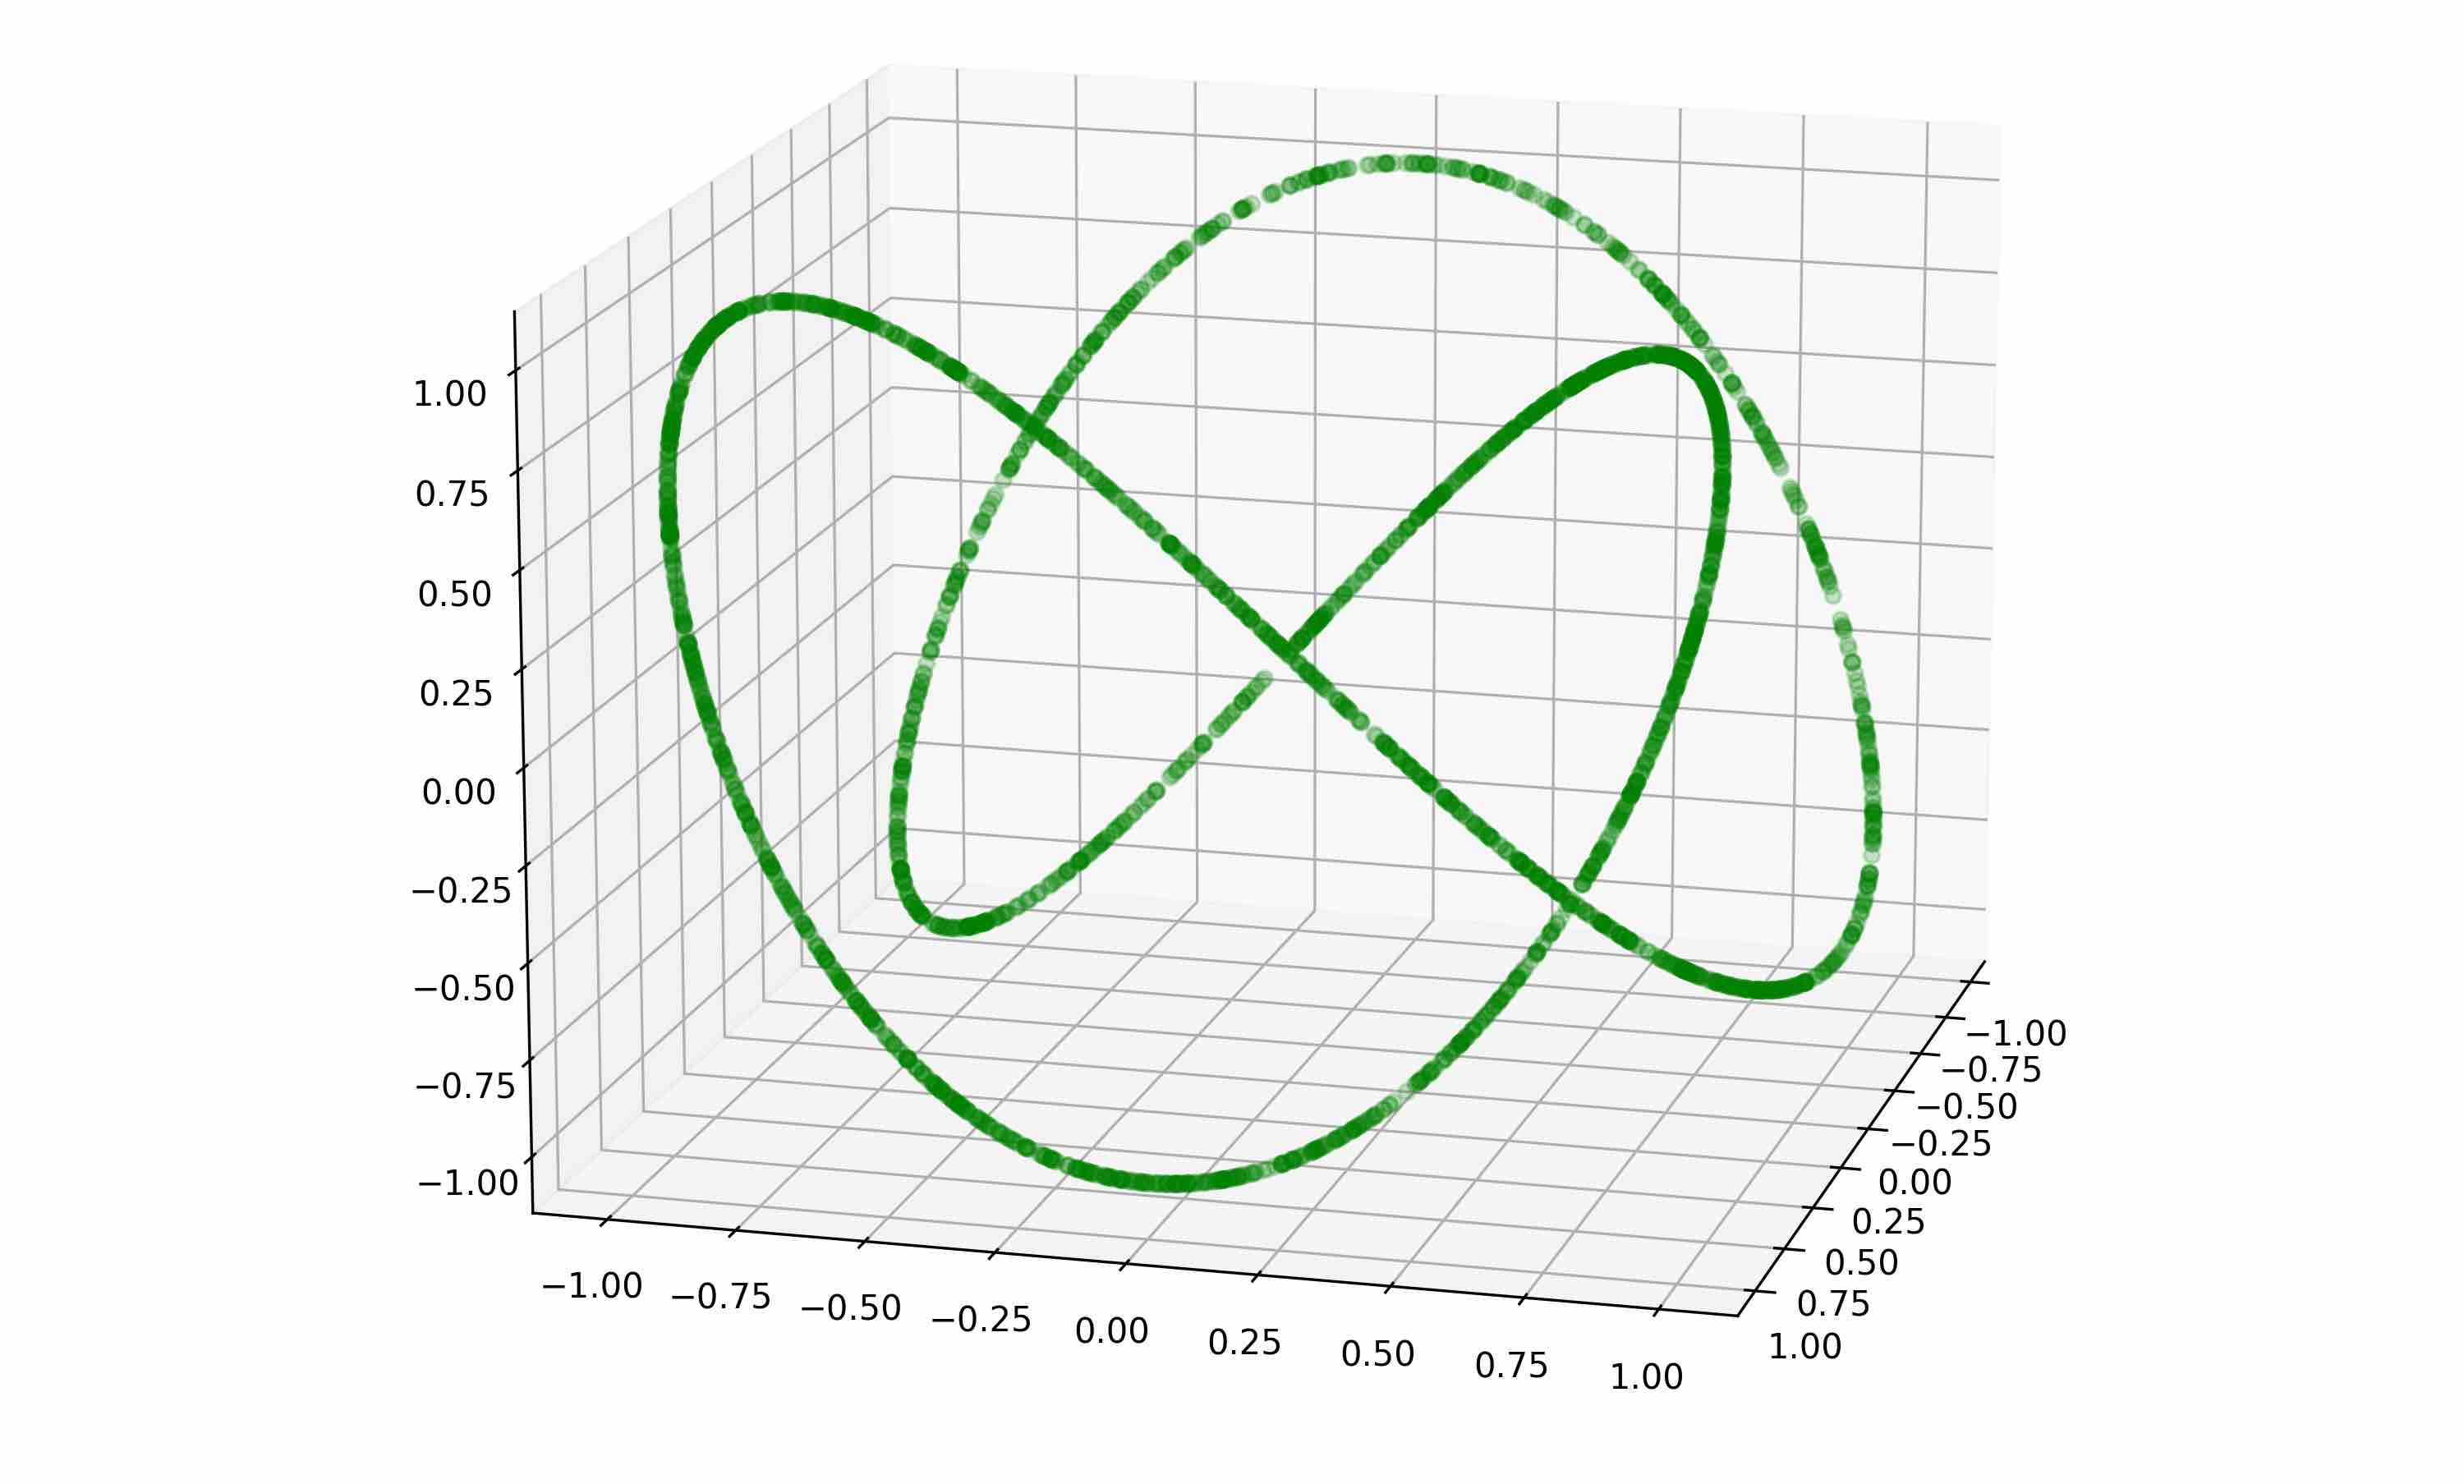
\includegraphics[width=.99\textwidth]{chapter3/figures/spaghetti.jpg}
       \caption{Projection of the spaghetti line on the first three dimensions.}
       \label{ch3:fig:line_samples}
   \end{minipage}
   \hspace{5mm}
   \begin{minipage}[t]{.45\textwidth}
       \centering
       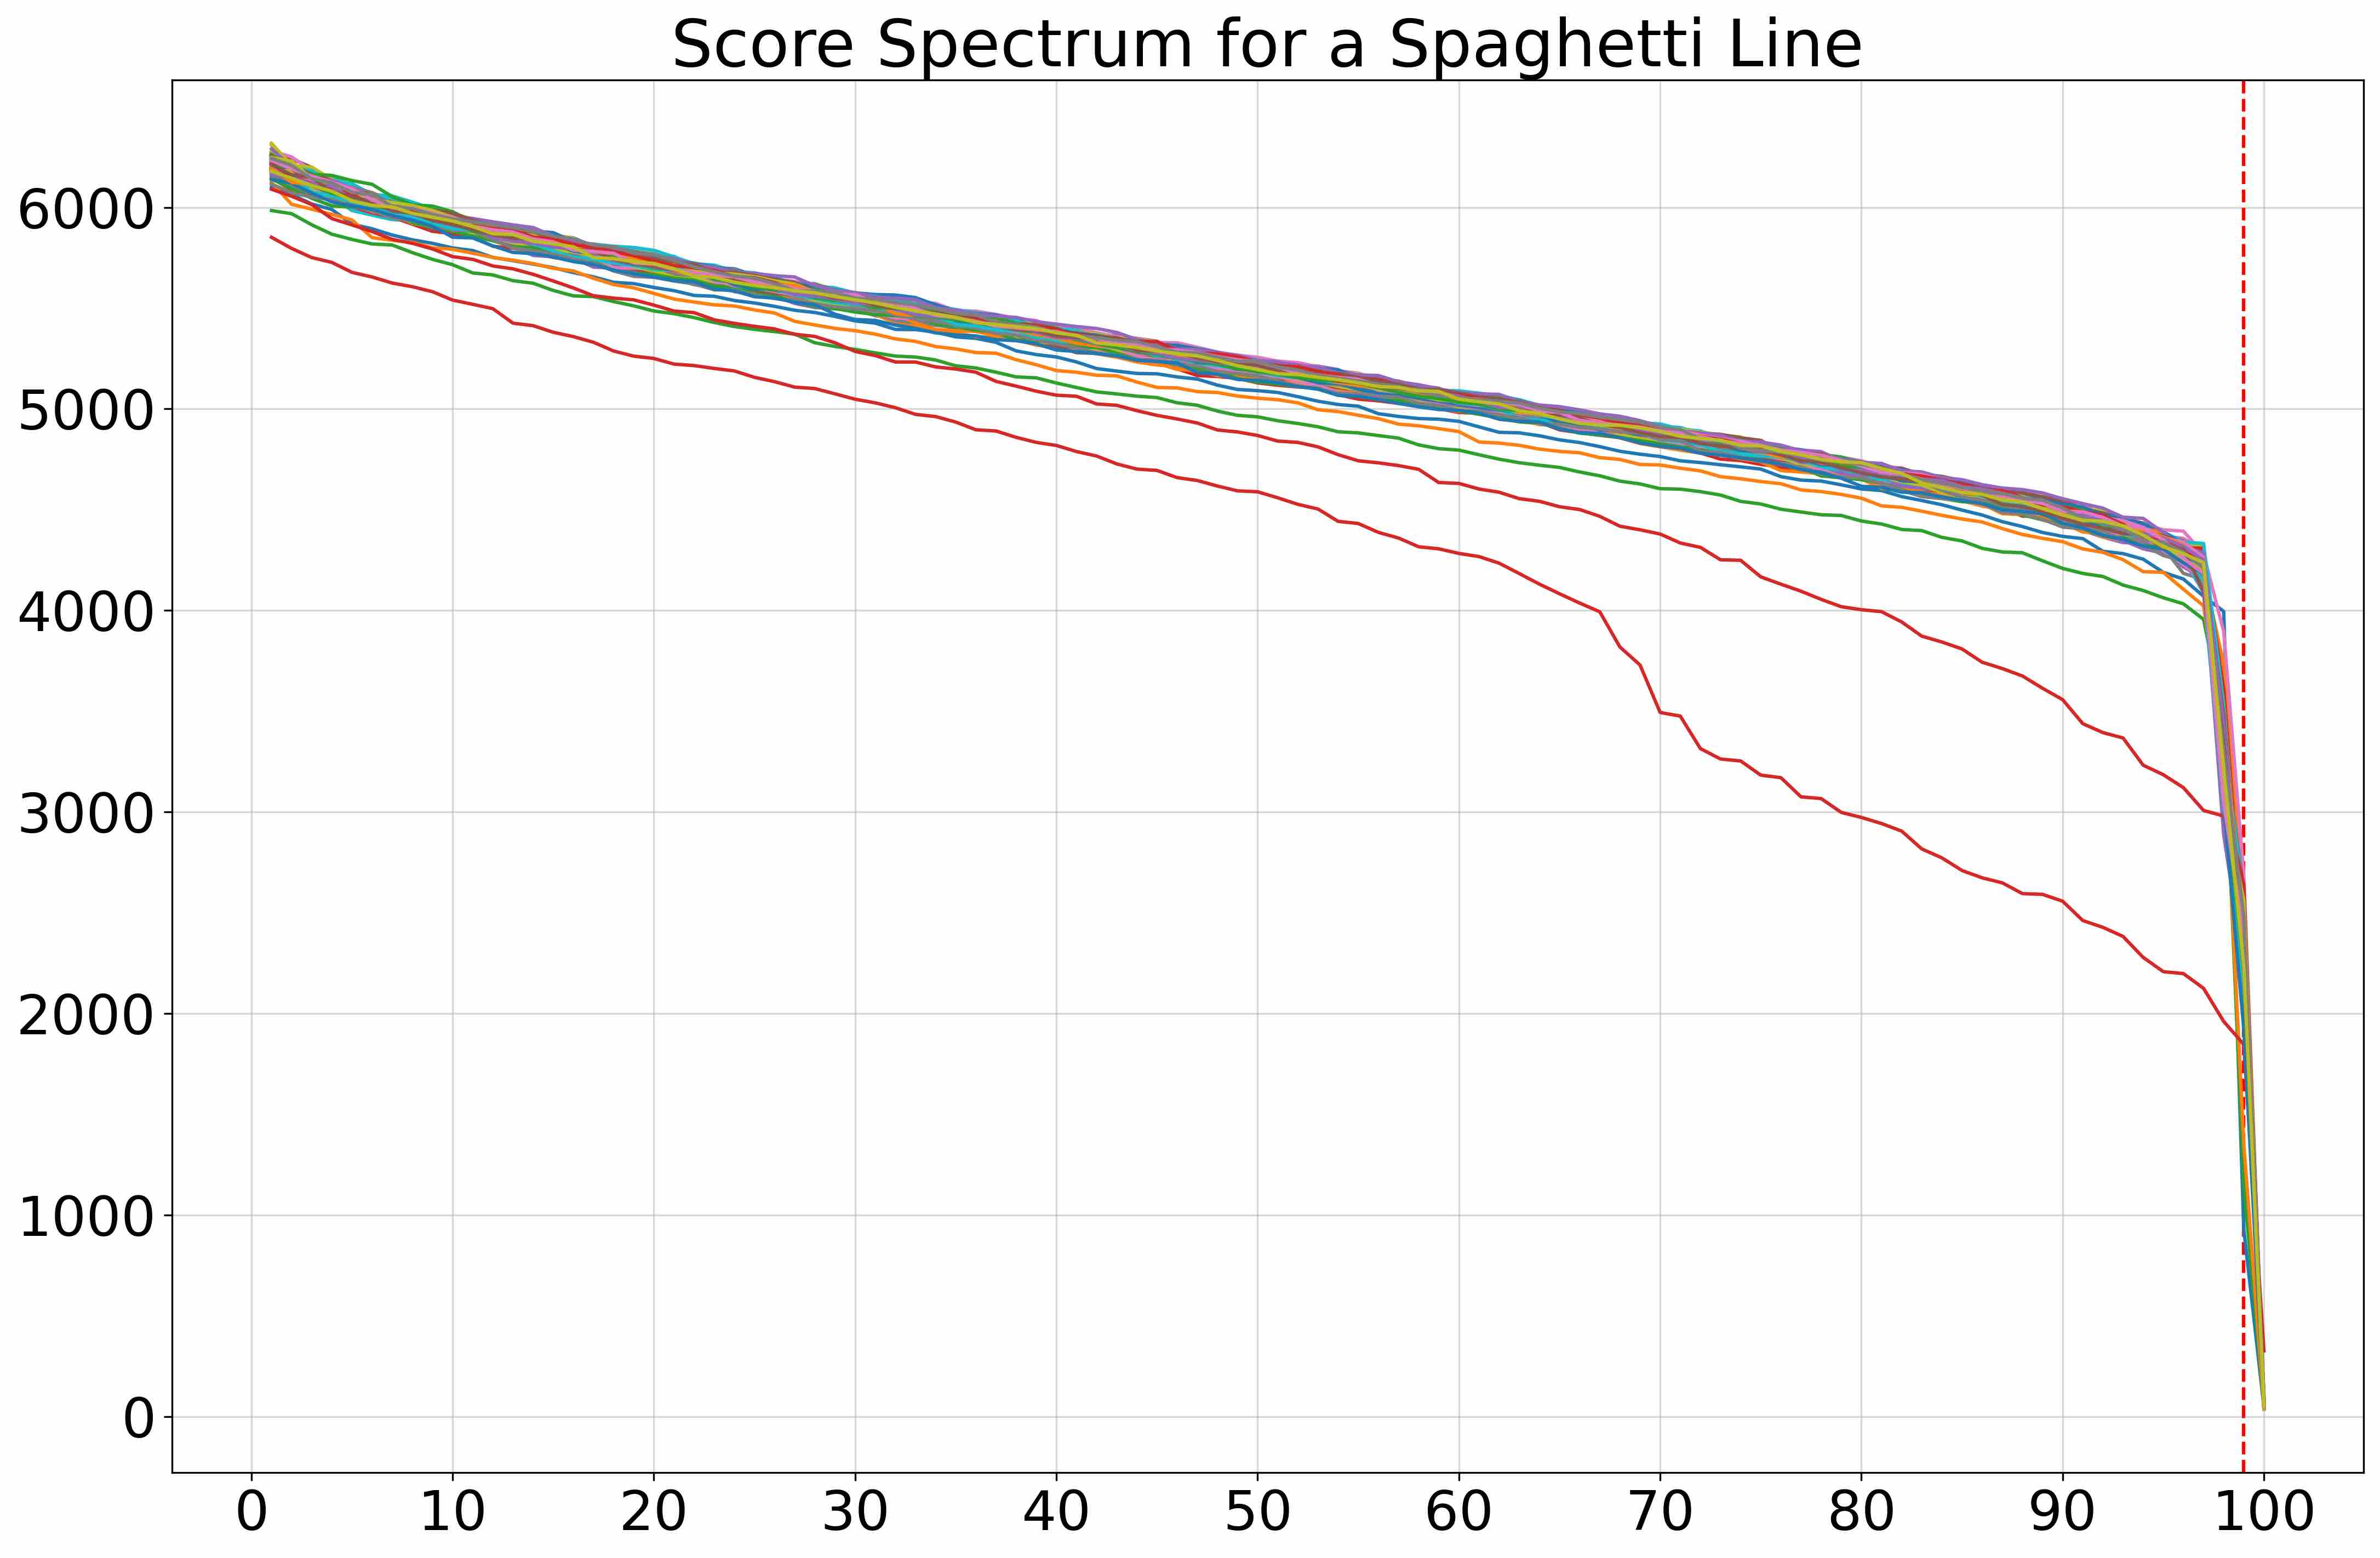
\includegraphics[width=.99\textwidth]{chapter3/figures/line_spectrum.jpg}
       \caption{Score spectrum of the spaghetti line. The last singular value clearly vanishes indicating that the intrinsic dimensionality of the manifold is equal to one.}
       \label{ch3:fig:line}
   \end{minipage}
   \end{figure}
   
   \begin{figure}[H]
   \begin{minipage}[t]{.45\textwidth}
       \centering
       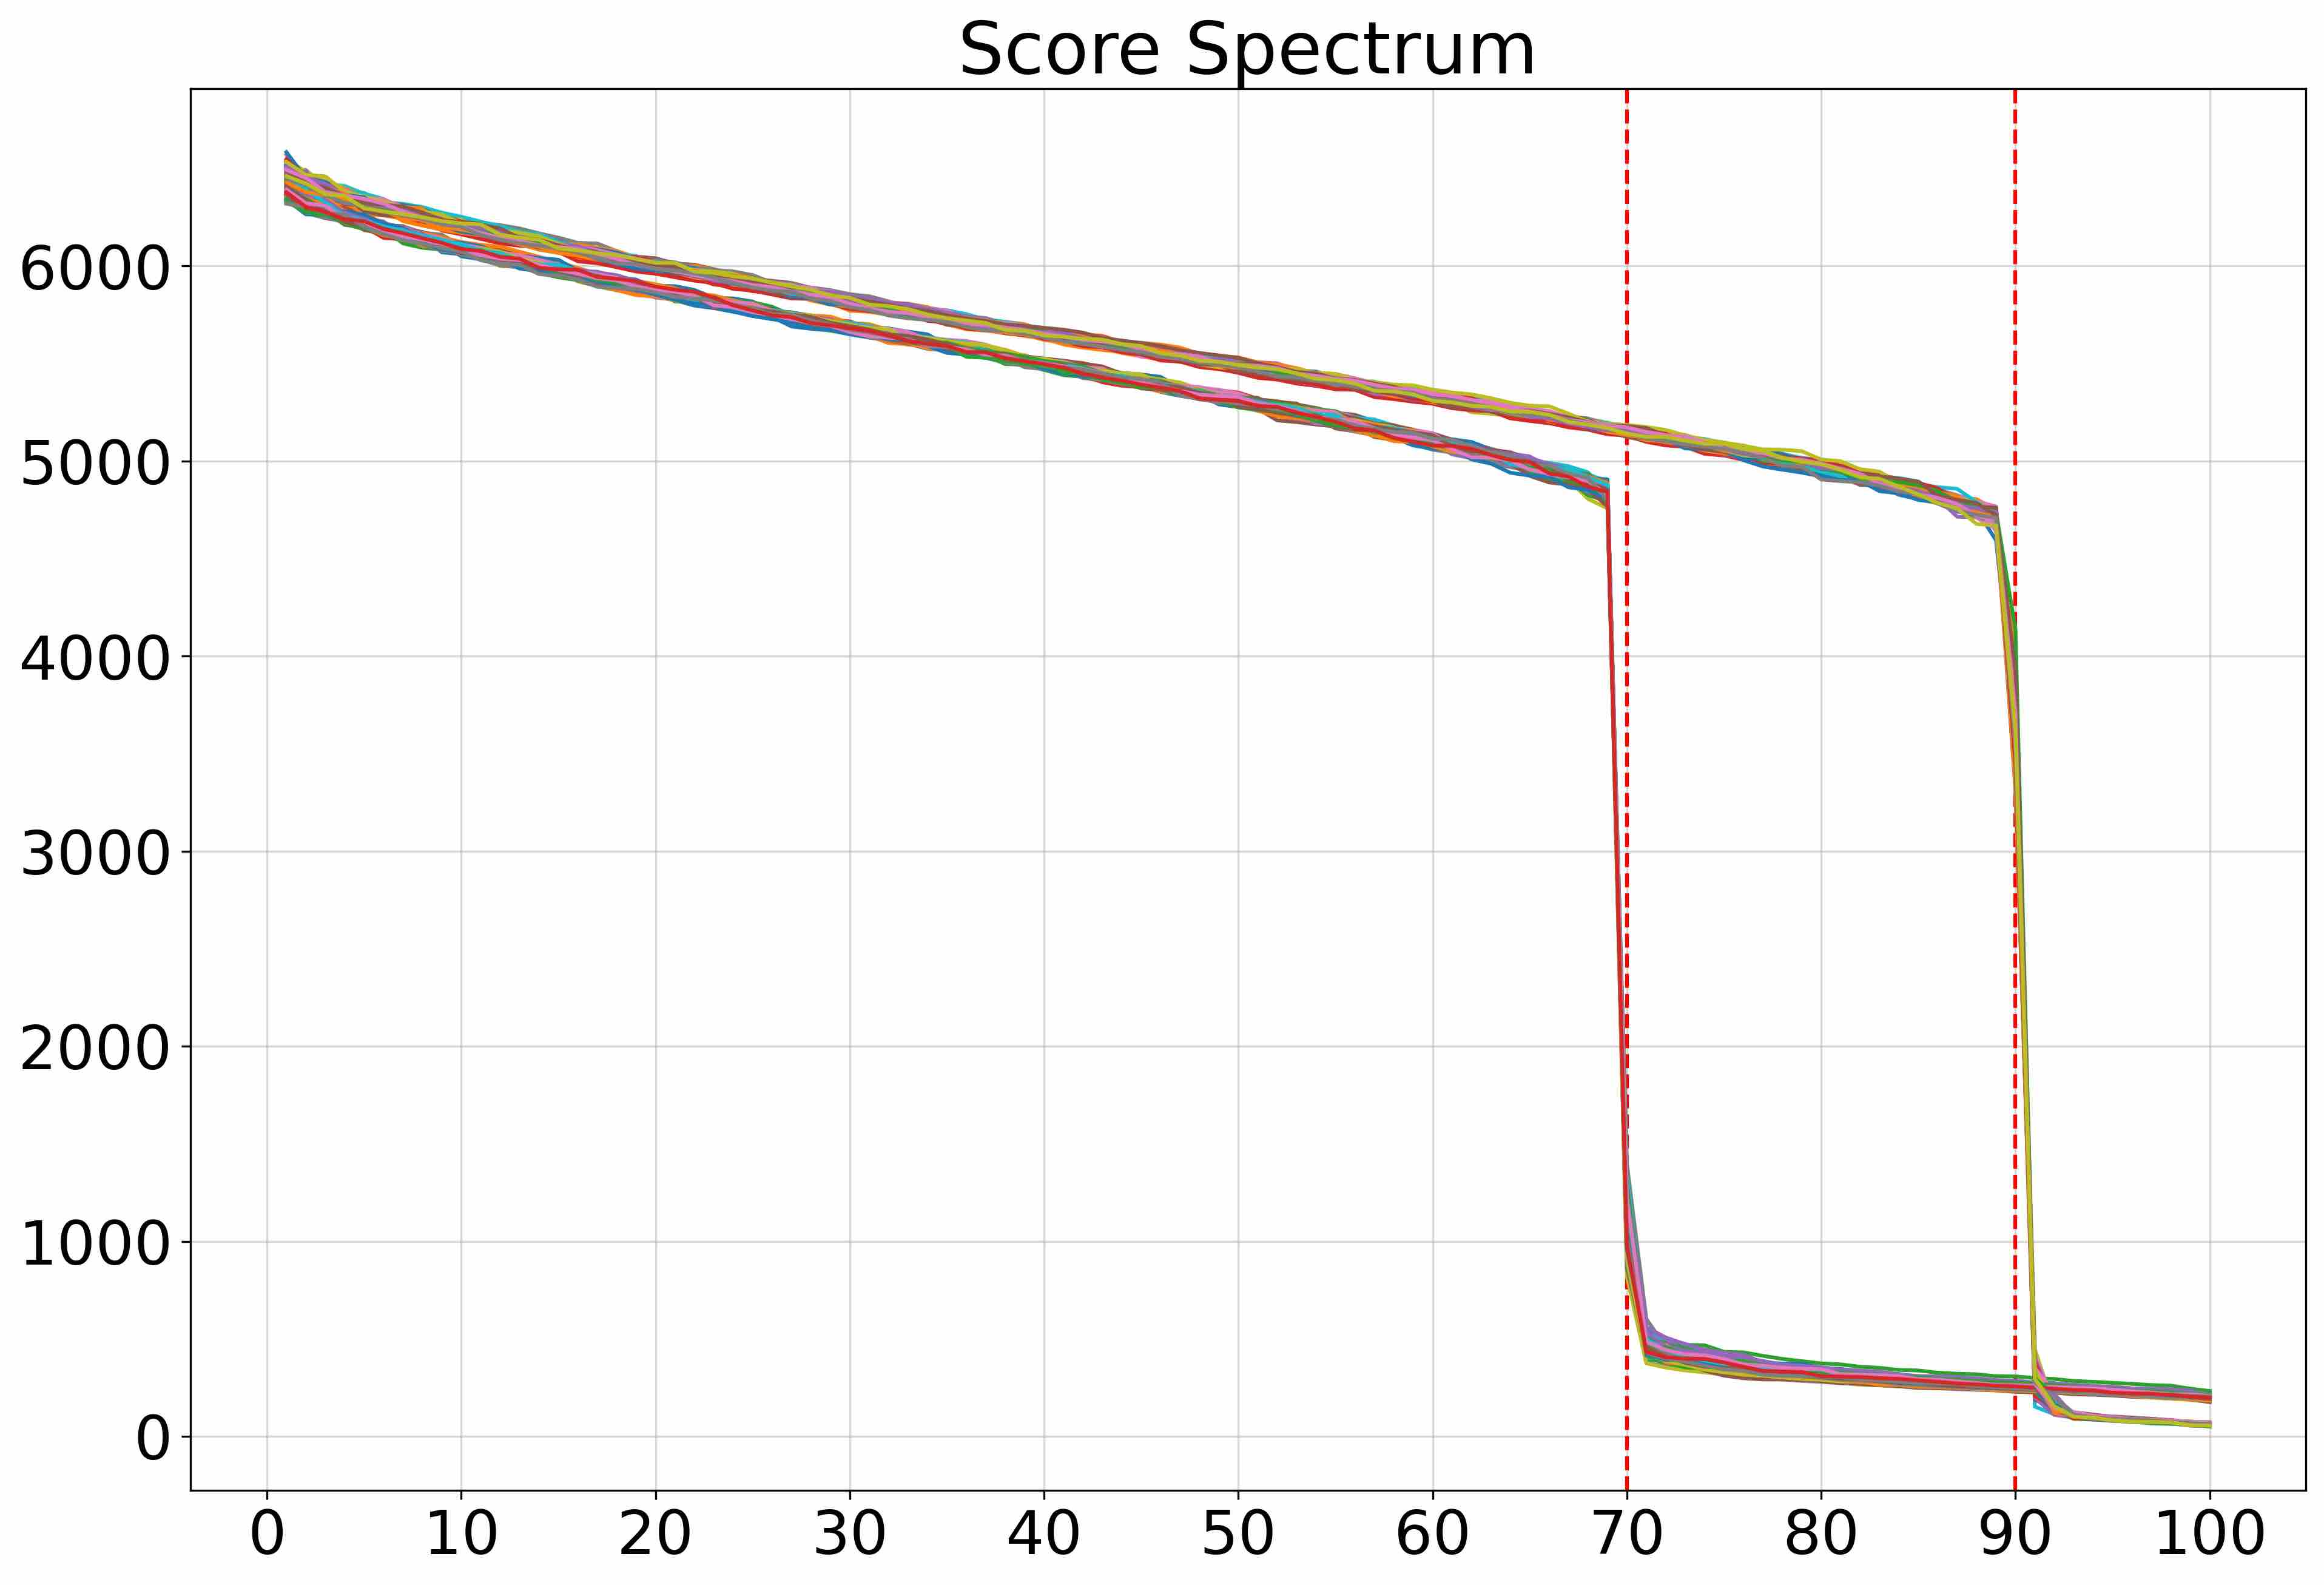
\includegraphics[width=\linewidth]{chapter3/figures/union_of_spheres_spectrum.jpg}
       \caption{Score spectrum for the union of $k$-spheres ($k_1=10, k_2=30$). The separated drops in the spectra clearly show that the data comes form the union of two manifolds of different dimensions.}
       \label{ch3:fig:unions_spectrum}
   \end{minipage}
   \hspace{5mm}
   \begin{minipage}[t]{.45\textwidth}
      \centering
       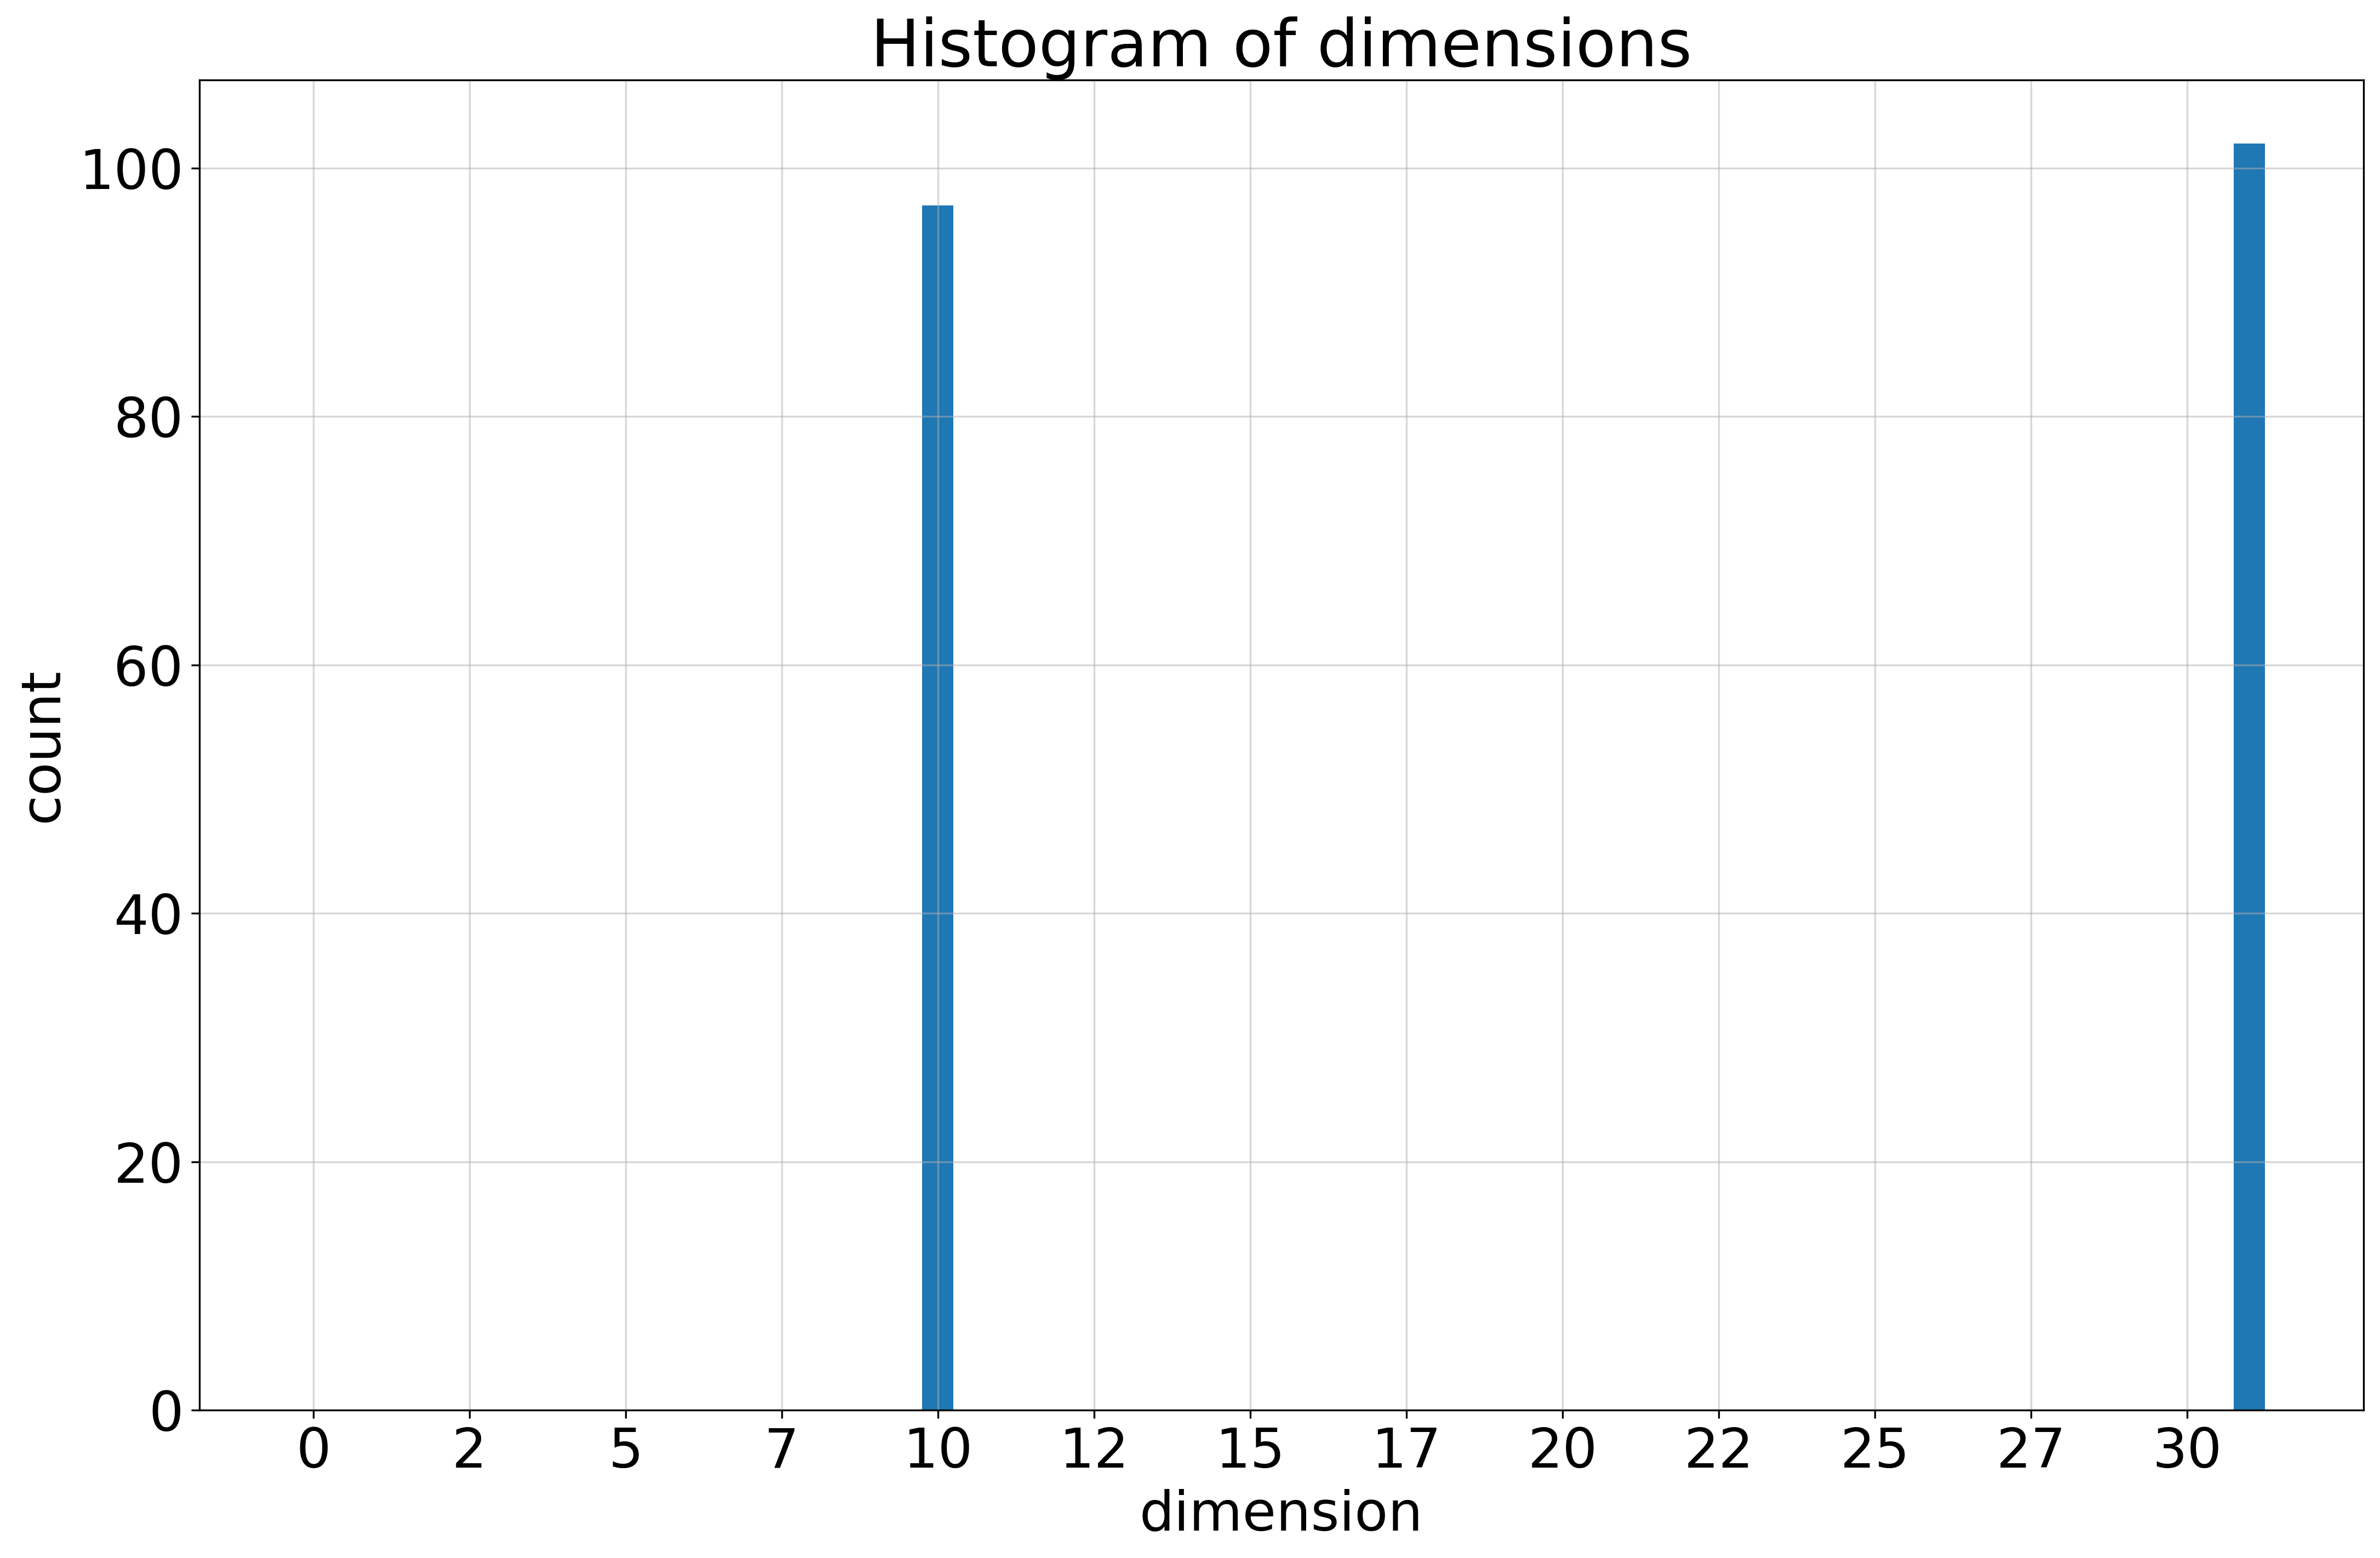
\includegraphics[width=0.99\textwidth]{chapter3/figures/union_of_spheres_dims.png}
       \caption{The histogram of estimated dimensions for the union of $k$-spheres ($k_1=10, k_2=30$). The counts are taken over estimates $\hat{k}(\textbf{x}_0^{(i)})$ at different points $\textbf{x}_0^{(i)}$.}
       \label{ch3:fig:union_dims}
   \end{minipage}
   \end{figure}
   
   
   \subsection{Synthetic Image Data}
   \label{ch3:appendix:additional_image}
   
   \begin{figure}[H]
   \centering
   \begin{minipage}[t]{.45\textwidth}
       \centering
       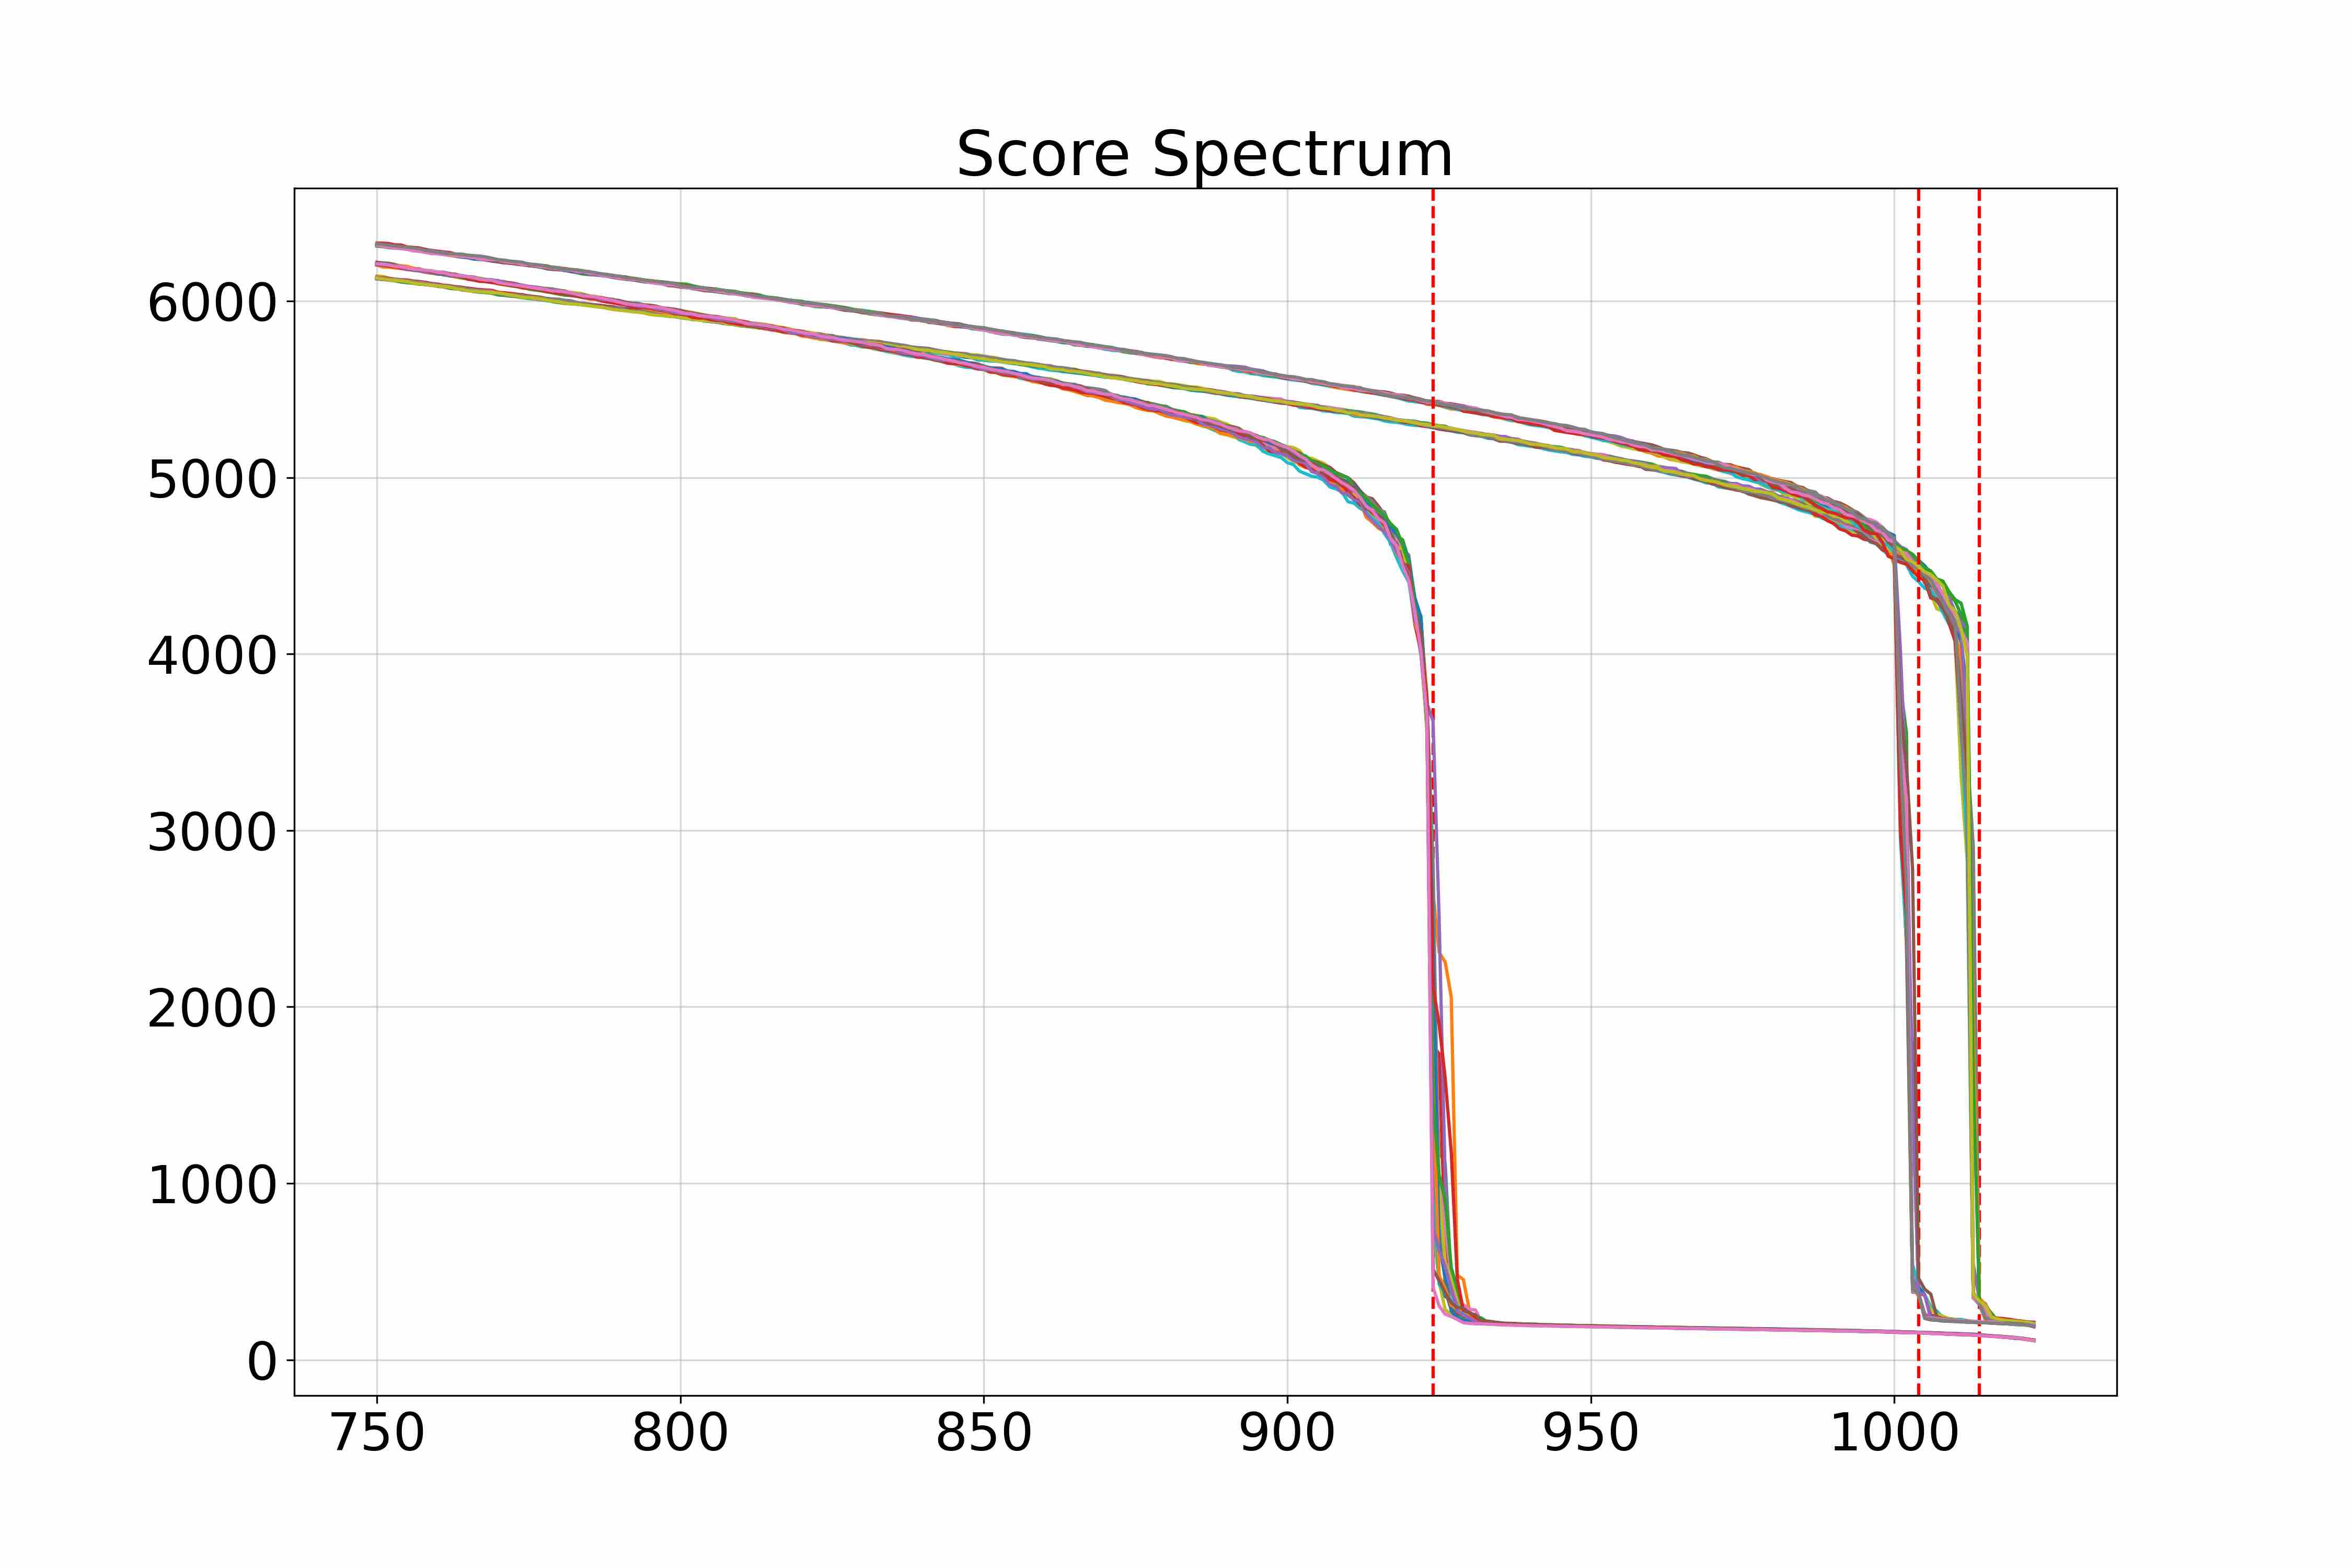
\includegraphics[width=.95\textwidth]{chapter3/figures/image_manifolds/squares_spectrum.jpg}\\
       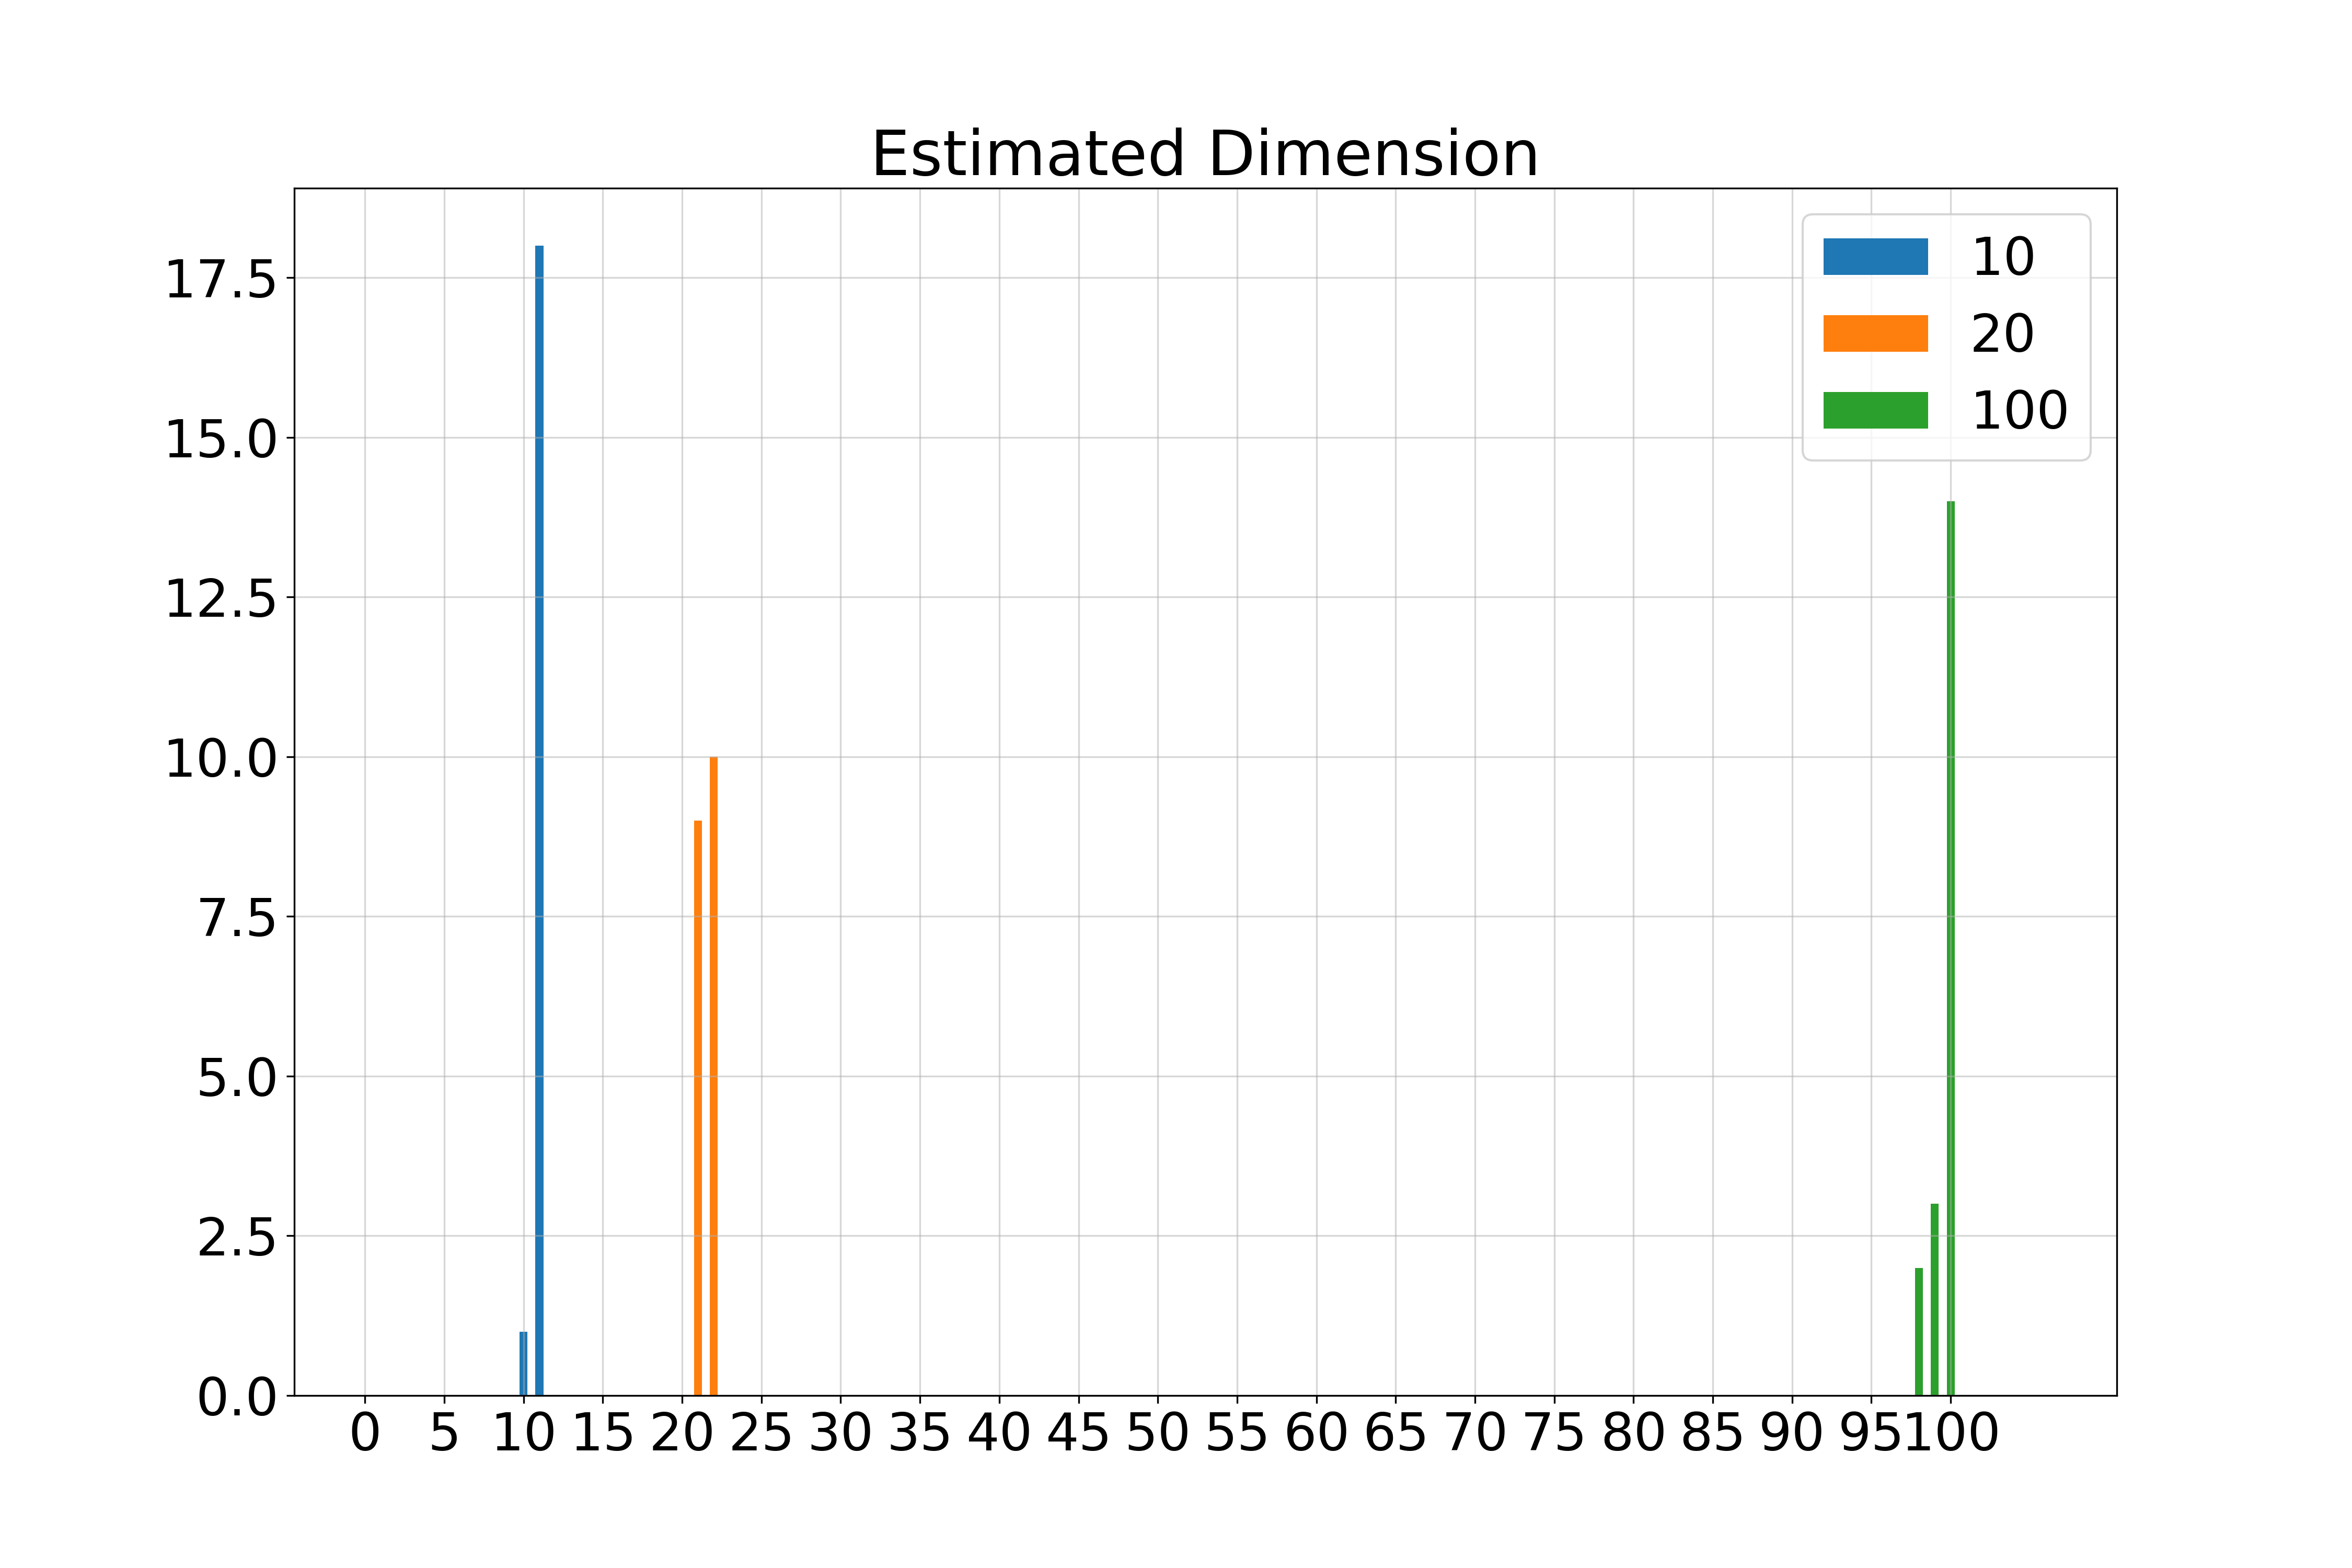
\includegraphics[width=.95\textwidth]{chapter3/figures/image_manifolds/squares_spectrum_adhoc.png}
       \caption{Score spectra and histogram of estimated dimension based on the score spectrum of the Squares image manifold of dimensions 10, 20 and 100.}
       \label{ch3:fig:squares_spectrum}
   \end{minipage}
   \hspace{10mm}
   \begin{minipage}[t]{.45\textwidth}
       \centering
       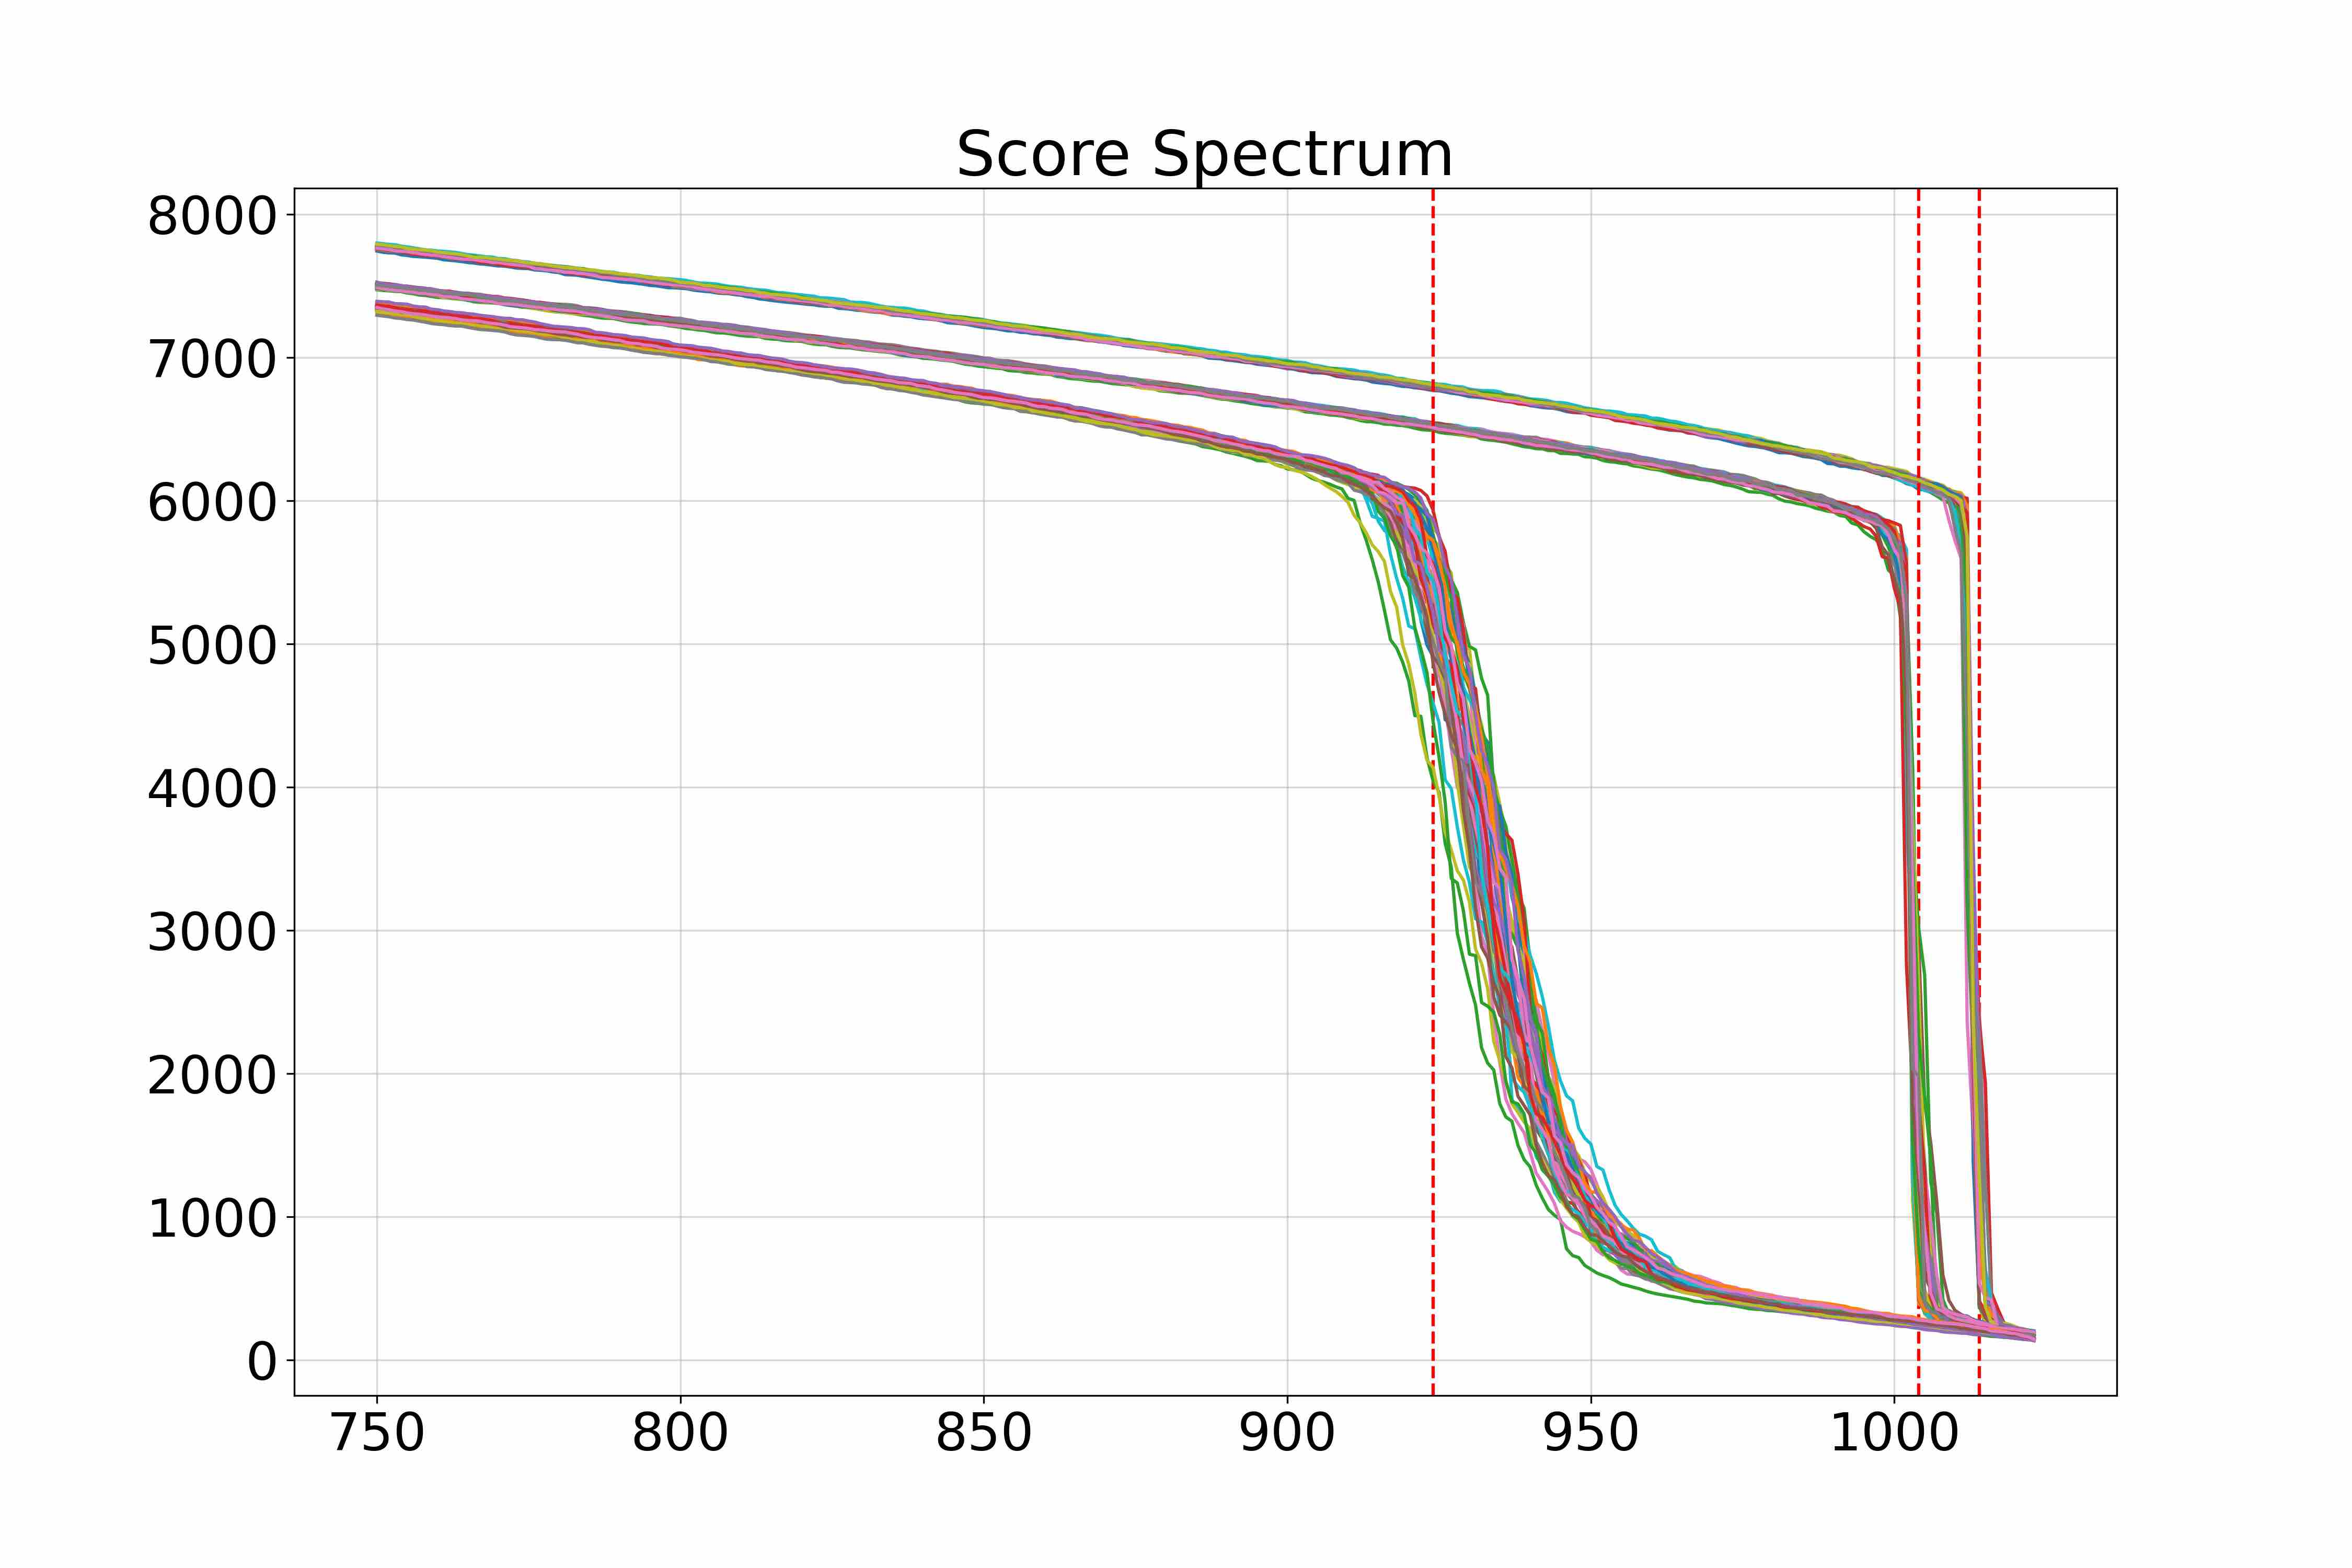
\includegraphics[width=.95\textwidth]{chapter3/figures/image_manifolds/gaussians_spectrum.jpg}\\
       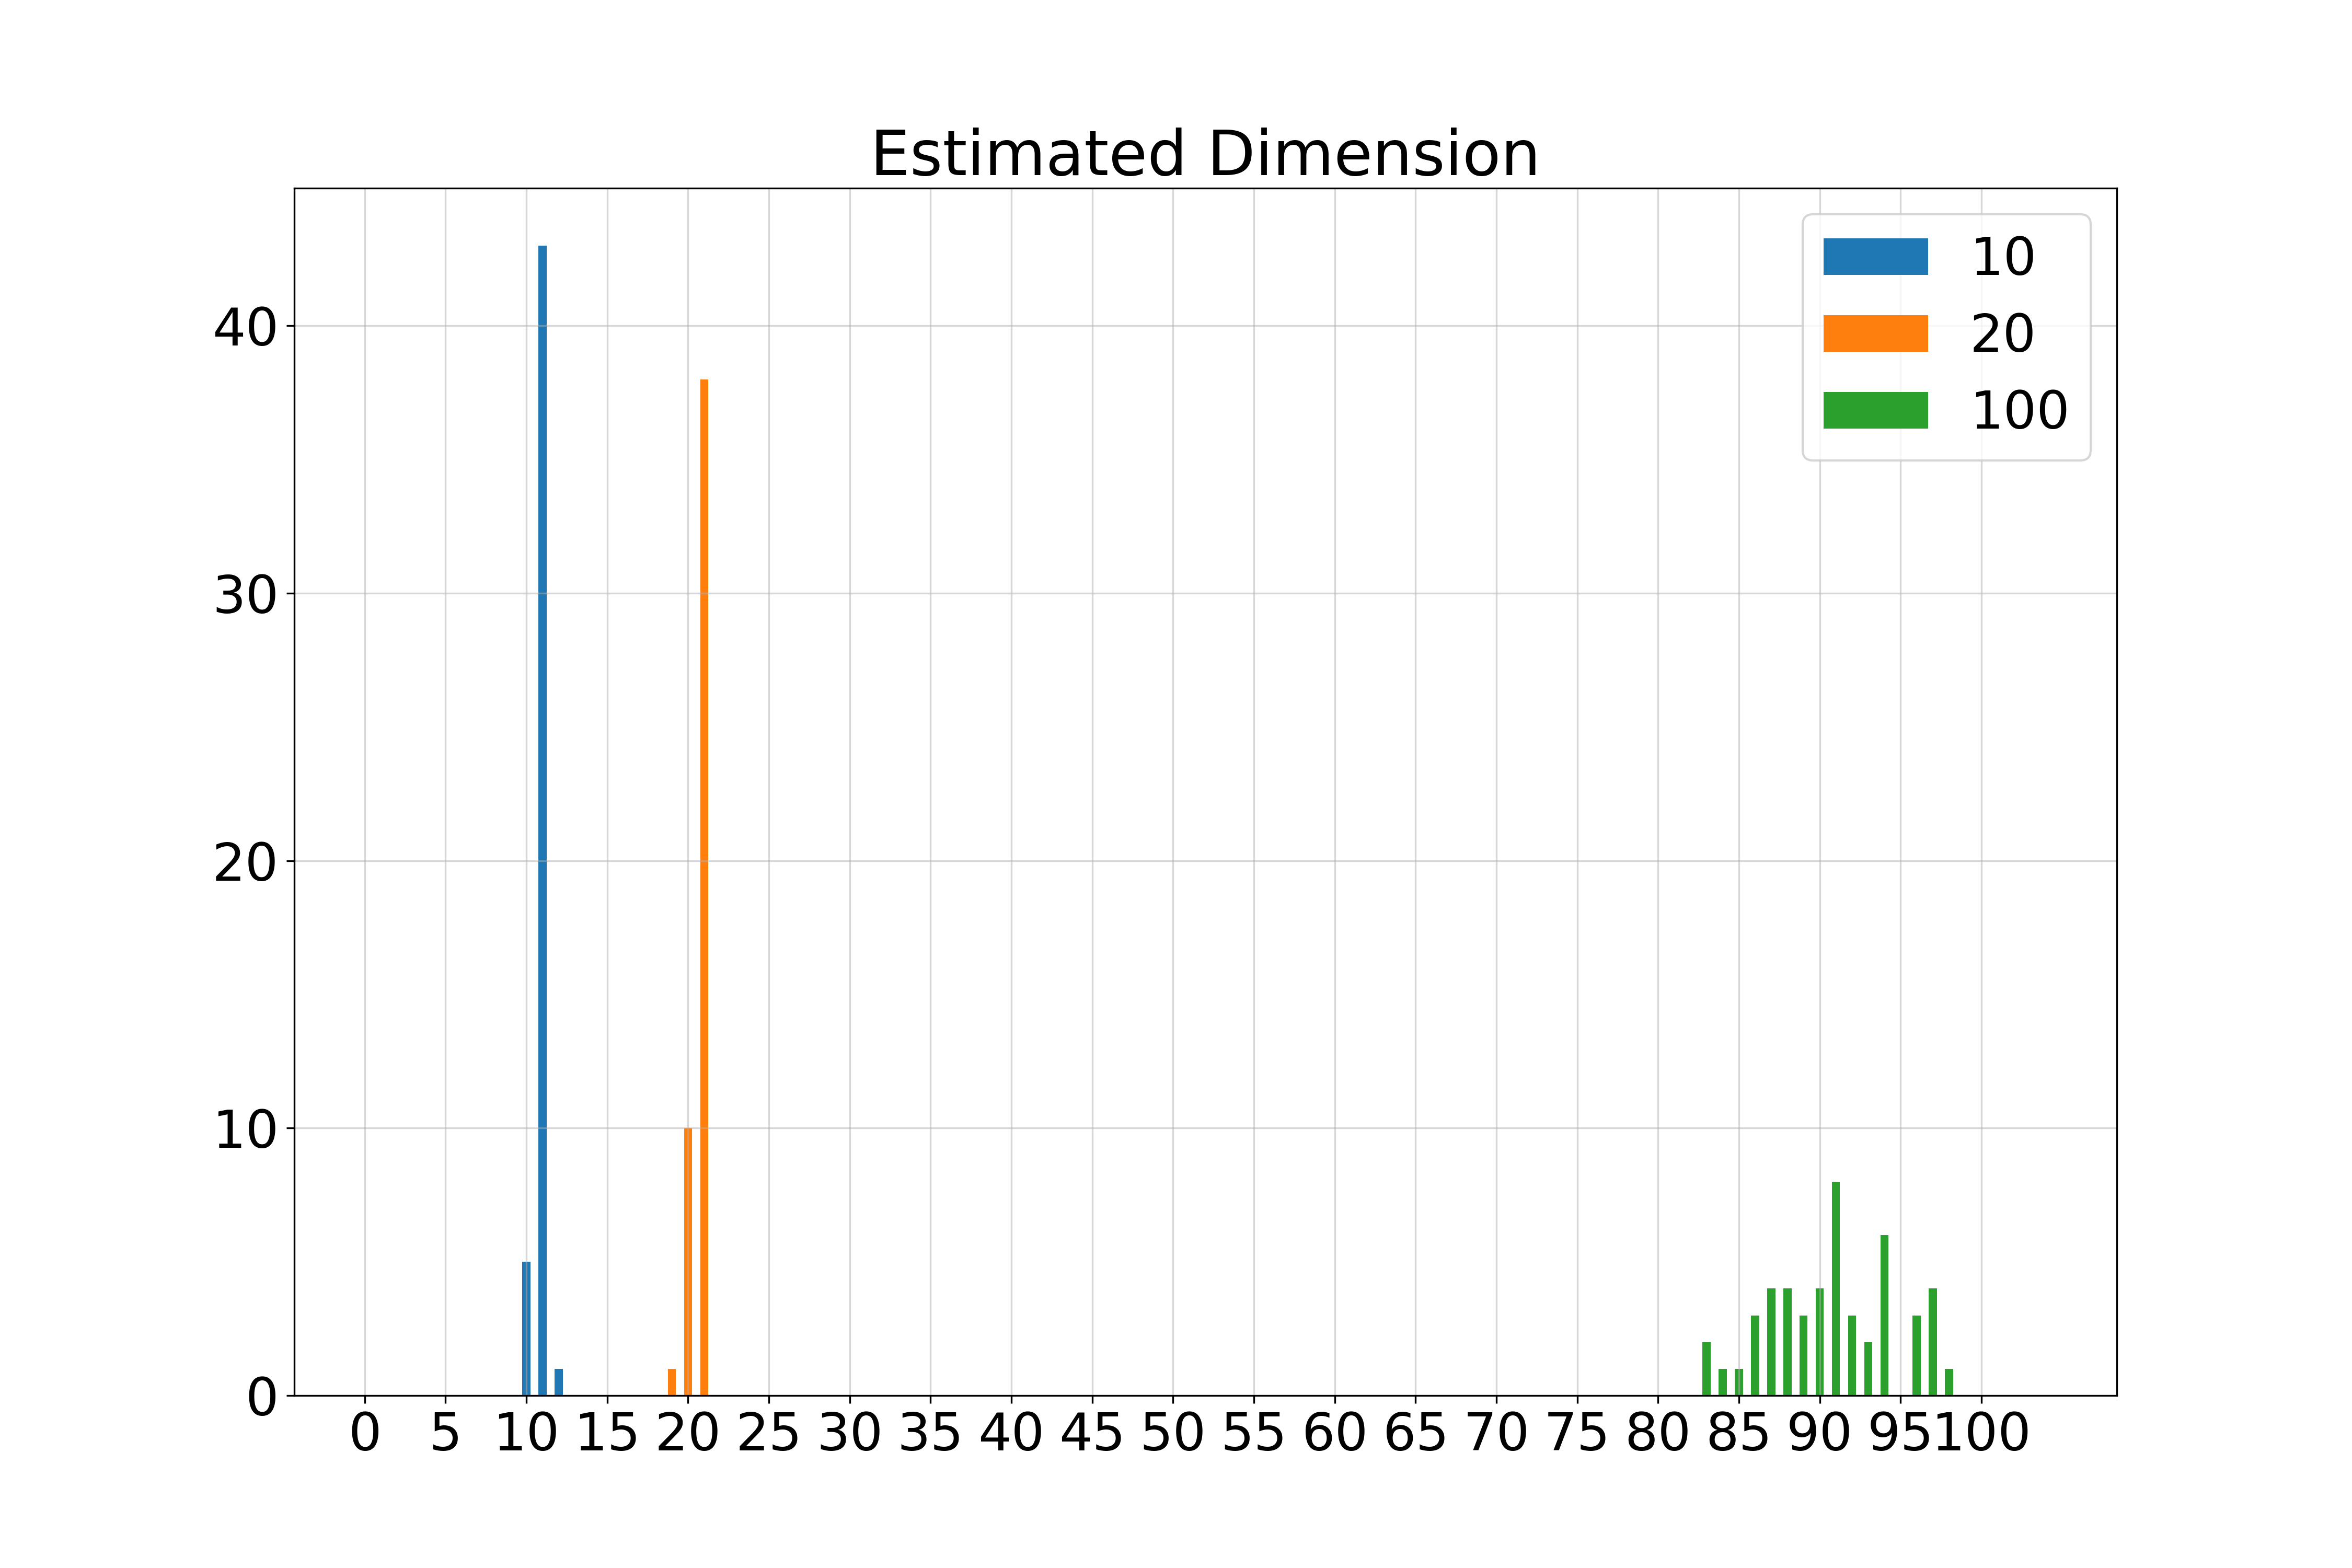
\includegraphics[width=.95\textwidth]{chapter3/figures/image_manifolds/gaussians_spectrum_adhoc.png}
       \caption{Score spectra and histogram of estimated dimension based on the score spectrum of the Gaussian blobs image manifold of dimensions 10, 20 and 100.}
       \label{ch3:fig:gaussians_spectrum}
   \end{minipage}
   \end{figure}
   
   
   \subsection{MNIST}
   \label{ch3:sec:Additional_Experimental_Results_for_MNIST}
   \begin{figure}[h!]
       \centering
       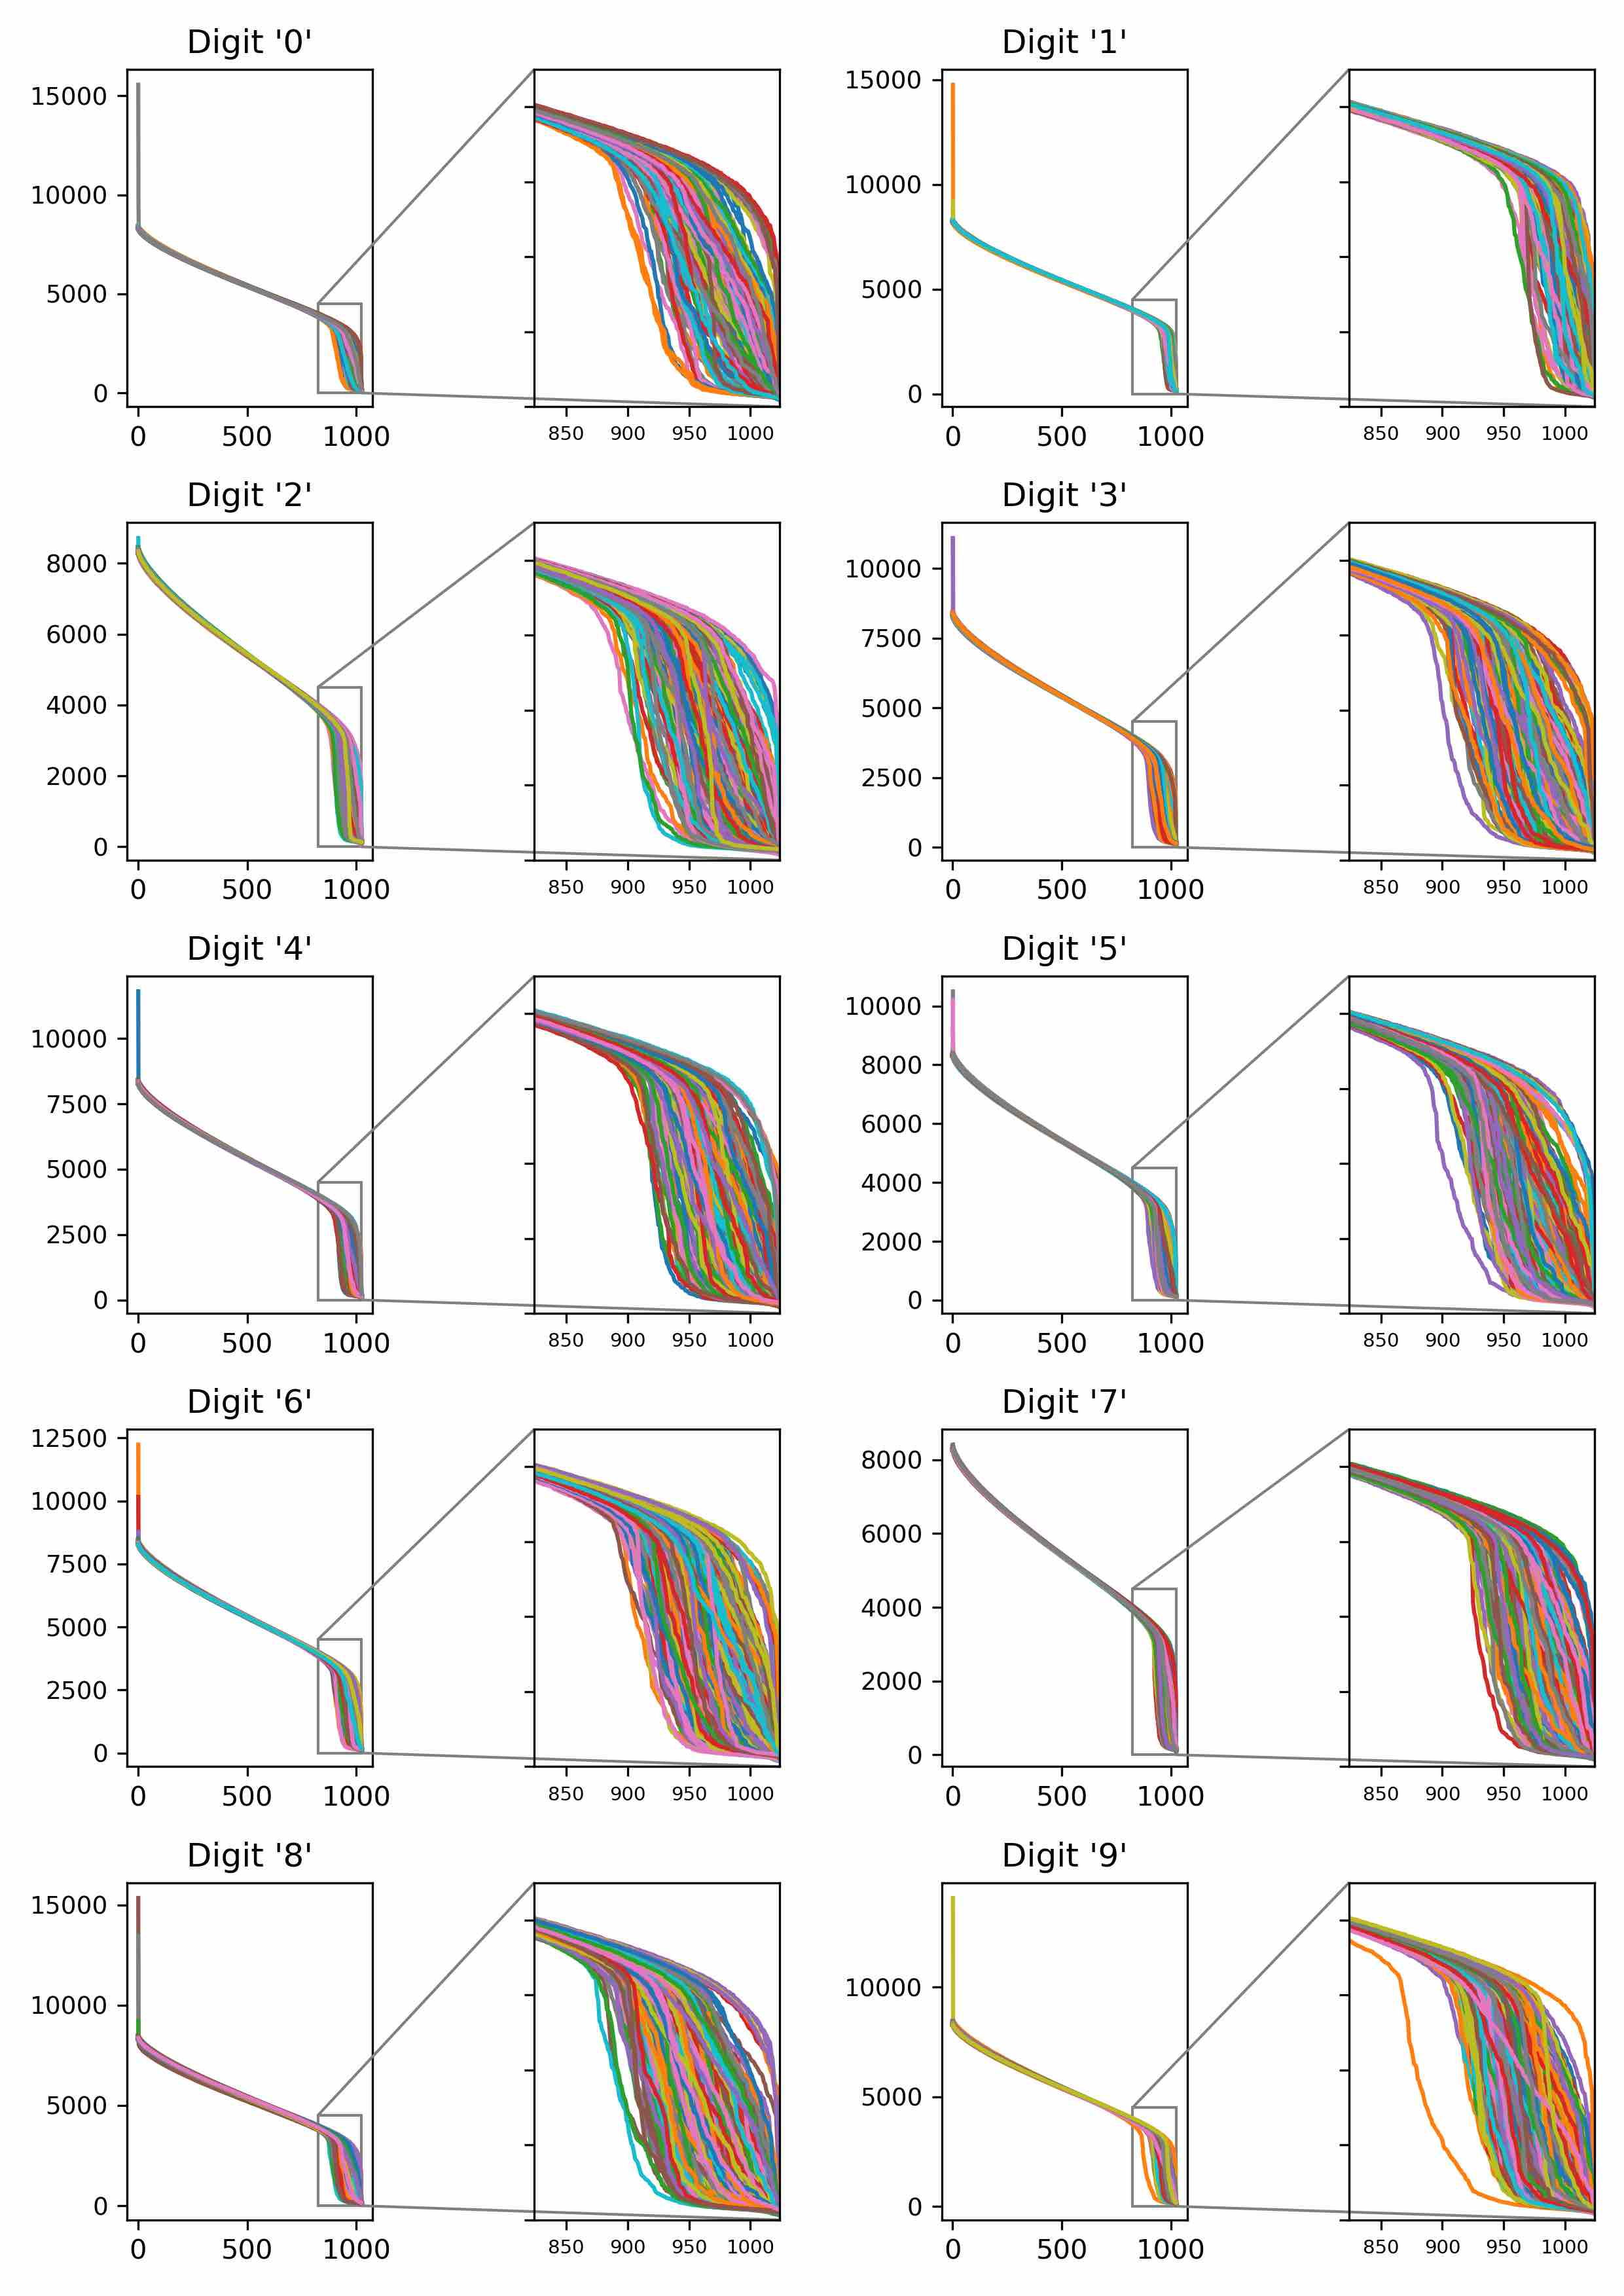
\includegraphics[width=0.9\textwidth]{chapter3/figures/image_manifolds/MNIST/mnist_spectrum_all_curves.jpg}
       \caption{MNIST score spectra for all digits}
       \label{ch3:fig:score_spectra_mnist_extended}
   \end{figure}
   
   In Figure \ref{ch3:fig:score_spectra_mnist_extended} we present $500$ score spectra evaluated at $500$ different instances for each digit. We observe that a considerable number of spectra indicate lower manifold dimension than the dimension documented in Table \ref{ch3:tab:estimated_mnist_dimensions}. This deviation can be attributed to amplified
   geometrical and statistical error at the respective evaluation points. 
   
   We choose the maximum estimated dimension as our conjecture of the intrinsic dimension under the premise that a collapse of the spectrum at a smaller dimension than the dimension of the normal space is extremely unlikely from a probabilistic standpoint.  However, it is feasible to encounter a spectrum collapse suggesting a higher normal space dimension, hence a lower intrinsic dimension, due to the intensified geometric and approximation error at the point of evaluation. It is noteworthy that our estimation strategy locates the drop at the position of the maximal gradient, a practice that may marginally inflate the intrinsic dimension estimate, as exemplified in the Squares and Gaussian blobs manifolds. Therefore, if our reported dimension for each MNIST digit is not precise, it is either a minor overestimation or a lower limit of the true dimension.
   
\section{Robustness analysis}
   \label{ch3:appendix:robust}
   \subsection{Robustness to score approximation error}
   As we discussed in the previous sections, our method is guaranteed to work given a perfect score approximation for sufficiently small $t$. However, in practice there will be an approximation error resulting from finite training data, limited model capacity and imperfect optimization. Therefore, we conduct an empirical analysis of the influence of the error in score approximation on the produced estimate of the dimension. We train a model $s_\theta$ on a uniform distribution on $25$-sphere and then we corrupt the output of the model with a Gaussian perturbation $e \sim \mathcal{N}(0, \sigma^2_e\textbf{I})$. Then, we produce score spectra by applying our method to the resulting corrupted scores. We repeat this experiment for different intensities of noise $\sigma_e$. We pick $\sigma_e$ so that the noise norm to score norm ratio $r = \mathbb{E}[\norm{e}] / \mathbb{E}_{x_{t_0} \sim p_{t_0}(\textbf{x}_{t_0} | \textbf{x}_0)}[\norm{s(\textbf{x}_{t_0} , t_0)}]$ has a prescribed value. We find that as we increase the intensity of noise singular values corresponding to the tangential component start to increase causing the gap in the score spectrum  to diminish. This is expected since the noise added to the score vectors has a tangential component.  However, for values of $r < 0.5$ our method is still producing a visible drop in the spectrum at the correct point. The results are presented in Figure \ref{ch3:fig:robustness_score}.
   
   \begin{figure}[h!]
       \centering
       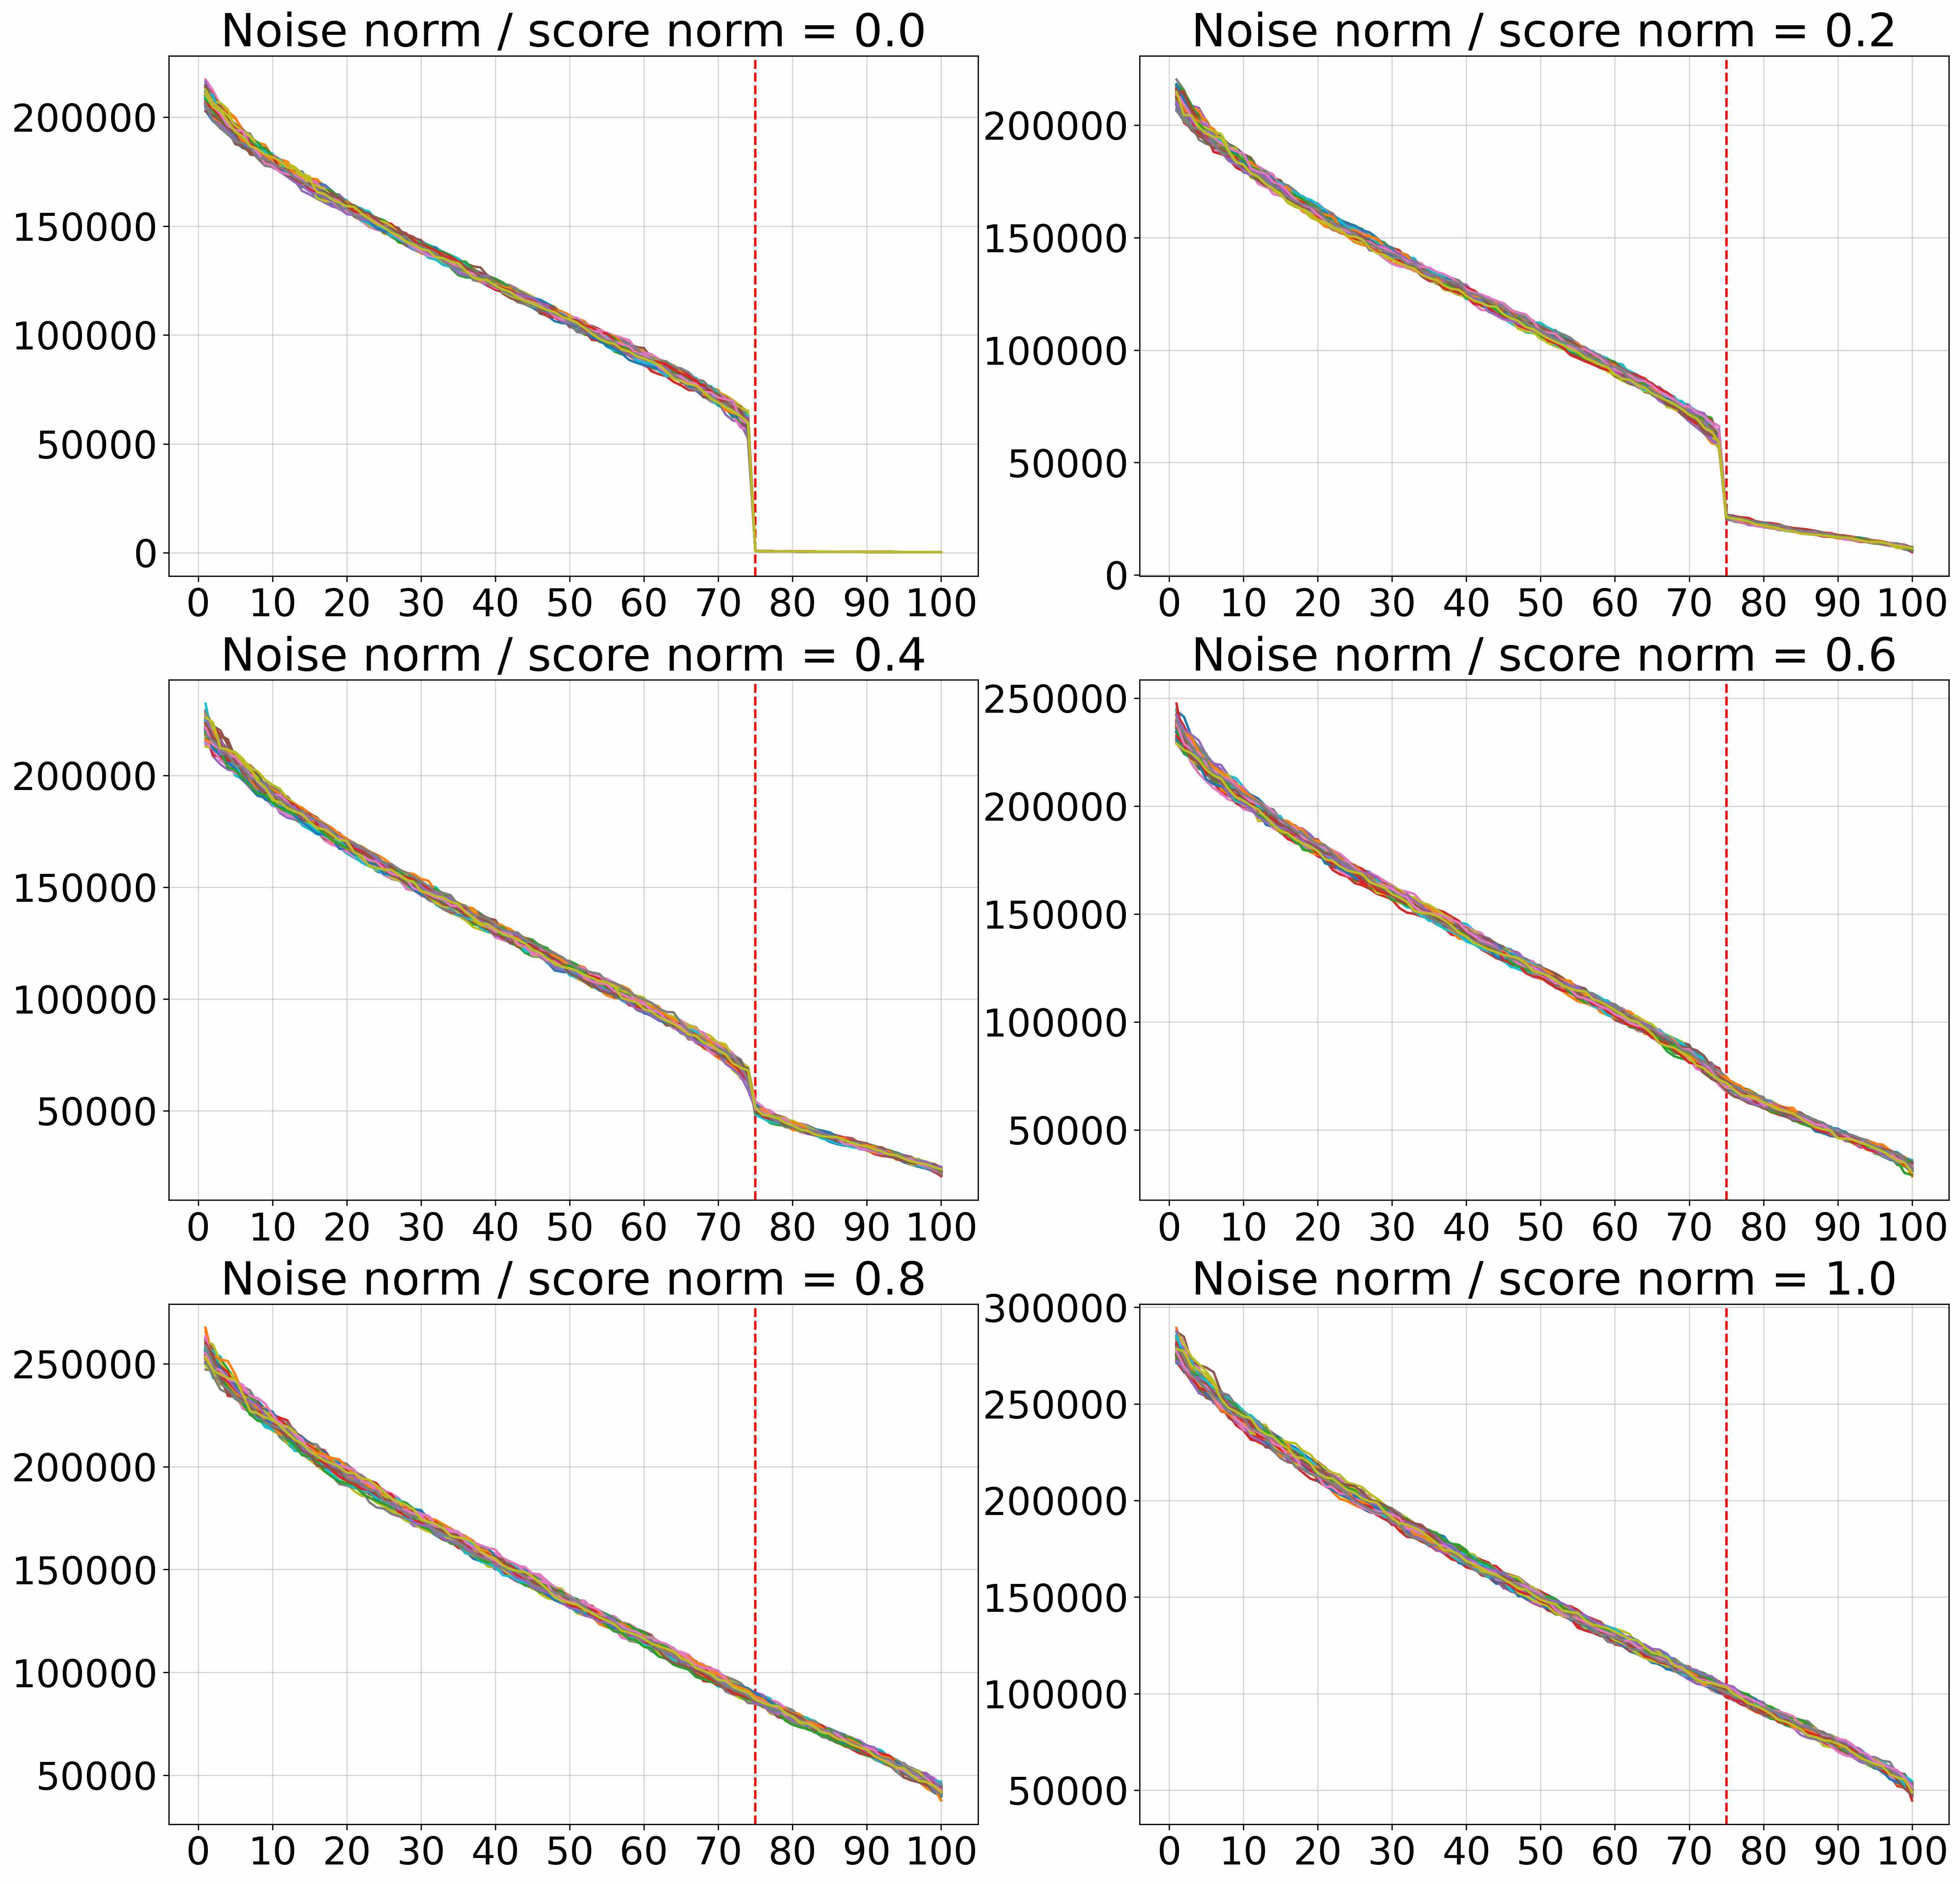
\includegraphics[width=\textwidth]{Chapter3/figures/robustness_score.jpg}
       \caption{Score spectra for noise corrupted score model on 25-sphere.}
       \label{ch3:fig:robustness_score}
   \end{figure}

   \subsection{Robustness to non-uniform distribution on the manifold}

   \begin{wraptable}{L}{0.6\textwidth}
       \begin{center}
       \small
       \begin{tabular}{ccccc}
       \toprule
       %& \multicolumn{3}{c}{Uniform distributions} &  \multicolumn{4}{c}{Non-uniform 10-sphere}\\
       & Uniform & $\alpha=1$ & $\alpha=0.75$ & $\alpha=0.5$  \\
       \midrule
       \multirow{1}{*}{Ground Truth} 
       &10 & 10 & 10  & 10    \\
       \midrule
       \multirow{1}{*}{Ours}
       &11 & 10 & 10  & 7 \\
       \midrule
       
       \multirow{1}{*}{MLE (m=5)}
       &9.61 & 5.37 & 4.83  & 4.12   \\
       \midrule
   
       \multirow{1}{*}{MLE (m=20)}
       &9.46 & 4.99 & 4.49  & 3.82 \\
       \midrule
   
       \multirow{1}{*}{Local PCA}
       & 11 & 5 & 4  & 3  \\
       \midrule
   
       \multirow{1}{*}{PPCA}
       & 11 & 11 & 11  & 11  \\
       
       \bottomrule
       \end{tabular}
       \end{center}
       \caption{Dimensionality detection for non-uniform distribution. For our method the maximum over pointwise estimates $\hat{k}(\textbf{x}_0)$ is considered.}
       \label{ch3:tbl:non_uniform}
   \end{wraptable}
   
   We examine the robustness to our method to non-unifomity in data distribution on the manifold surface. Under perfect score approximation and sufficiently small $t_0$ our method is guaranteed to work, but we conduct an empirical study to investigate the behaviour in the presence of score approximation error and $t_0 > 0$ used in practice in diffusion models. We consider a $k$-sphere and sample the surface of the sphere in a non-uniform fashion. We obtain points on the $k$-sphere by sampling vectors $\pmb \theta$ of $k-1$ angles (in radians) from a Gaussian distribution $\mathcal{N}(0, \alpha \mathbf{I})$, where $\alpha \in \mathbb{R}$ is a constant that determines the degree of non-uniformity. Then, we embed the resulting points via a random isometry in a 100 dimensional ambient space. We sample $n=1000$ points $\textbf{x}_0^{(j)}$ from the manifold and at each point we estimate the dimensionality $\hat{k}(\textbf{x}_0^{(j)})$ via the score spectrum. The pointwise estimates are presented in Figure \ref{ch3:fig:non_uniform} and final estimates are shown in Table \ref{ch3:tbl:non_uniform}. For values of $\alpha \in \{1, 0.75\}$, we can still obtain an accurate estimate of the dimension if we take $\hat{k} = \max_{j=1,...,1000} \hat{k}(\textbf{x}_0^{(j)})$ the maximum over point-wise estimates. For an extremely concentrated distribution with $\alpha = 0.5$ the method underestimates the dimension, which indicates that the tangential component of the score was not approximately constant in the neighborhoods used to sample the scores. This problem could be further mitigated by approximating the score closer to the manifold and using smaller sampling neighborhoods (i.e. for smaller $t_0$) or sampling more points $\textbf{x}_0^{(j)}$. Notice that taking the maximum over $\hat{k}(\textbf{x}_0^{(j)})$ is theoretically justified (as long as we assume we are dealing with a connected manifold) since our method can underestimate due to geometric or approximation error (cf. sections \ref{ch3:sec:theory} and \ref{ch3:sec:limitations}, but it is unlikely to significantly overestimate.

   \begin{figure*}
    \begin{minipage}[t]{0.5\textwidth}
        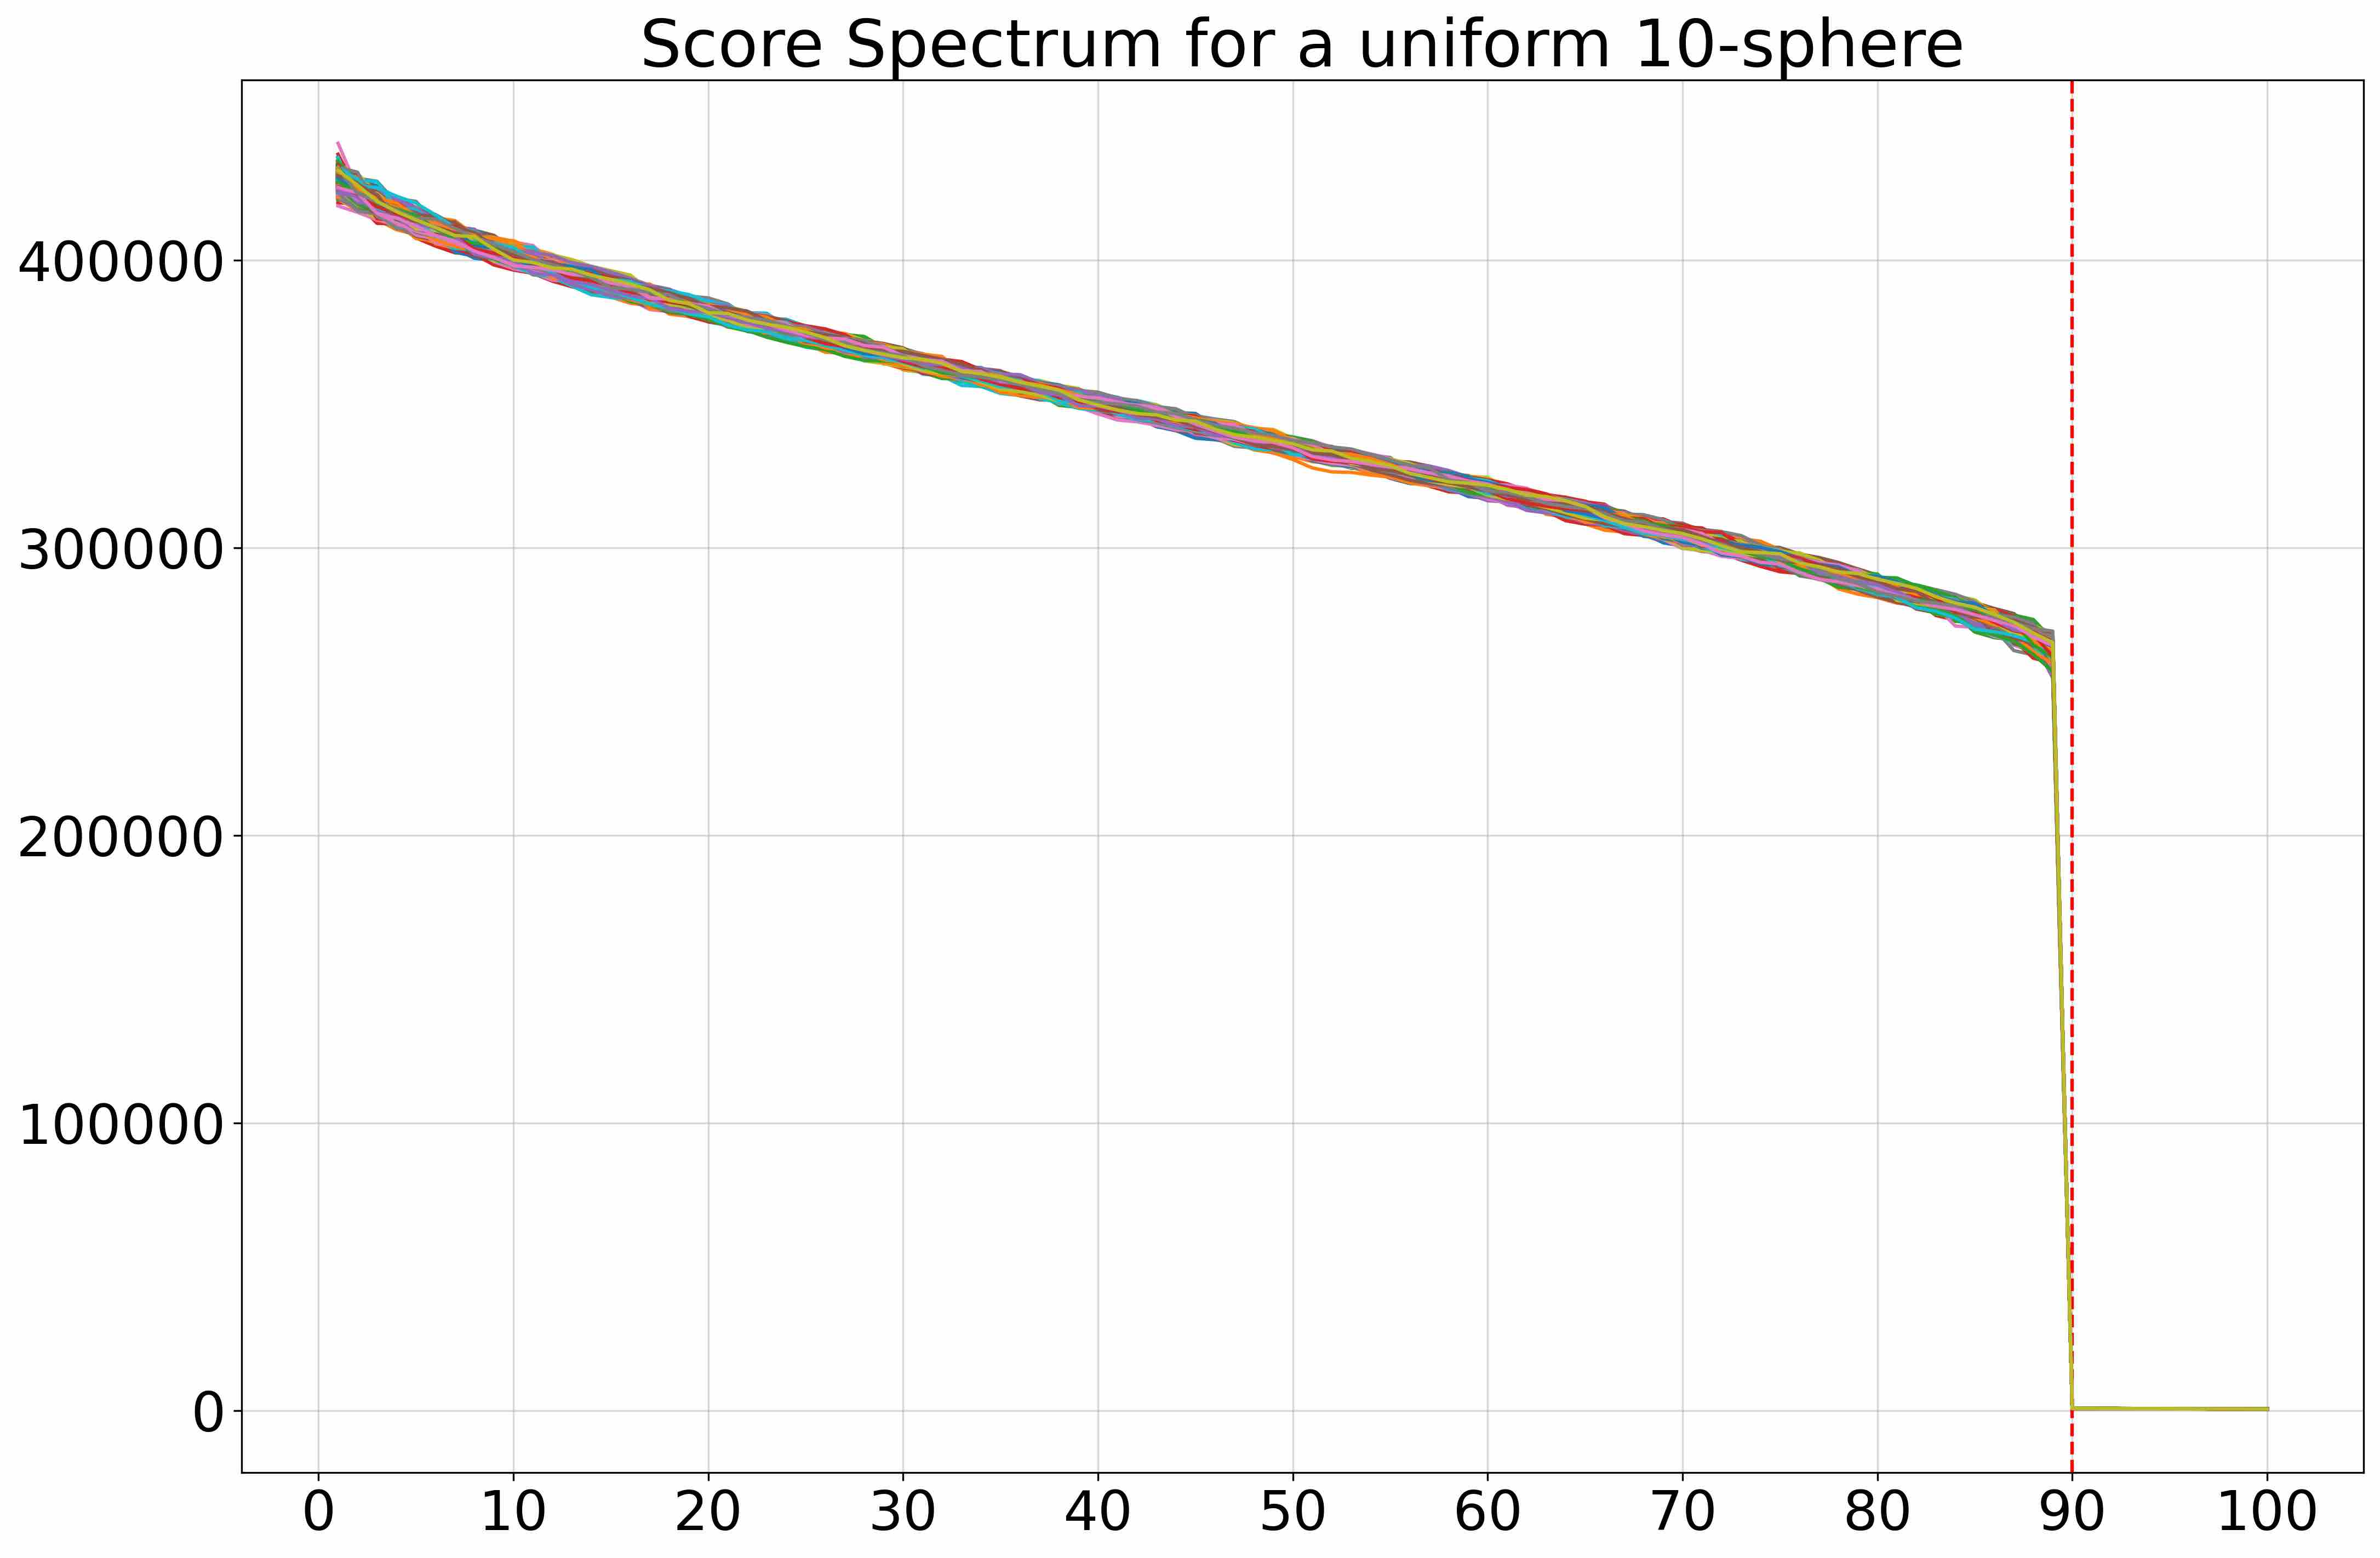
\includegraphics[width=0.95\linewidth]{chapter3/figures/non_uniform/spectrum_0.jpg}
        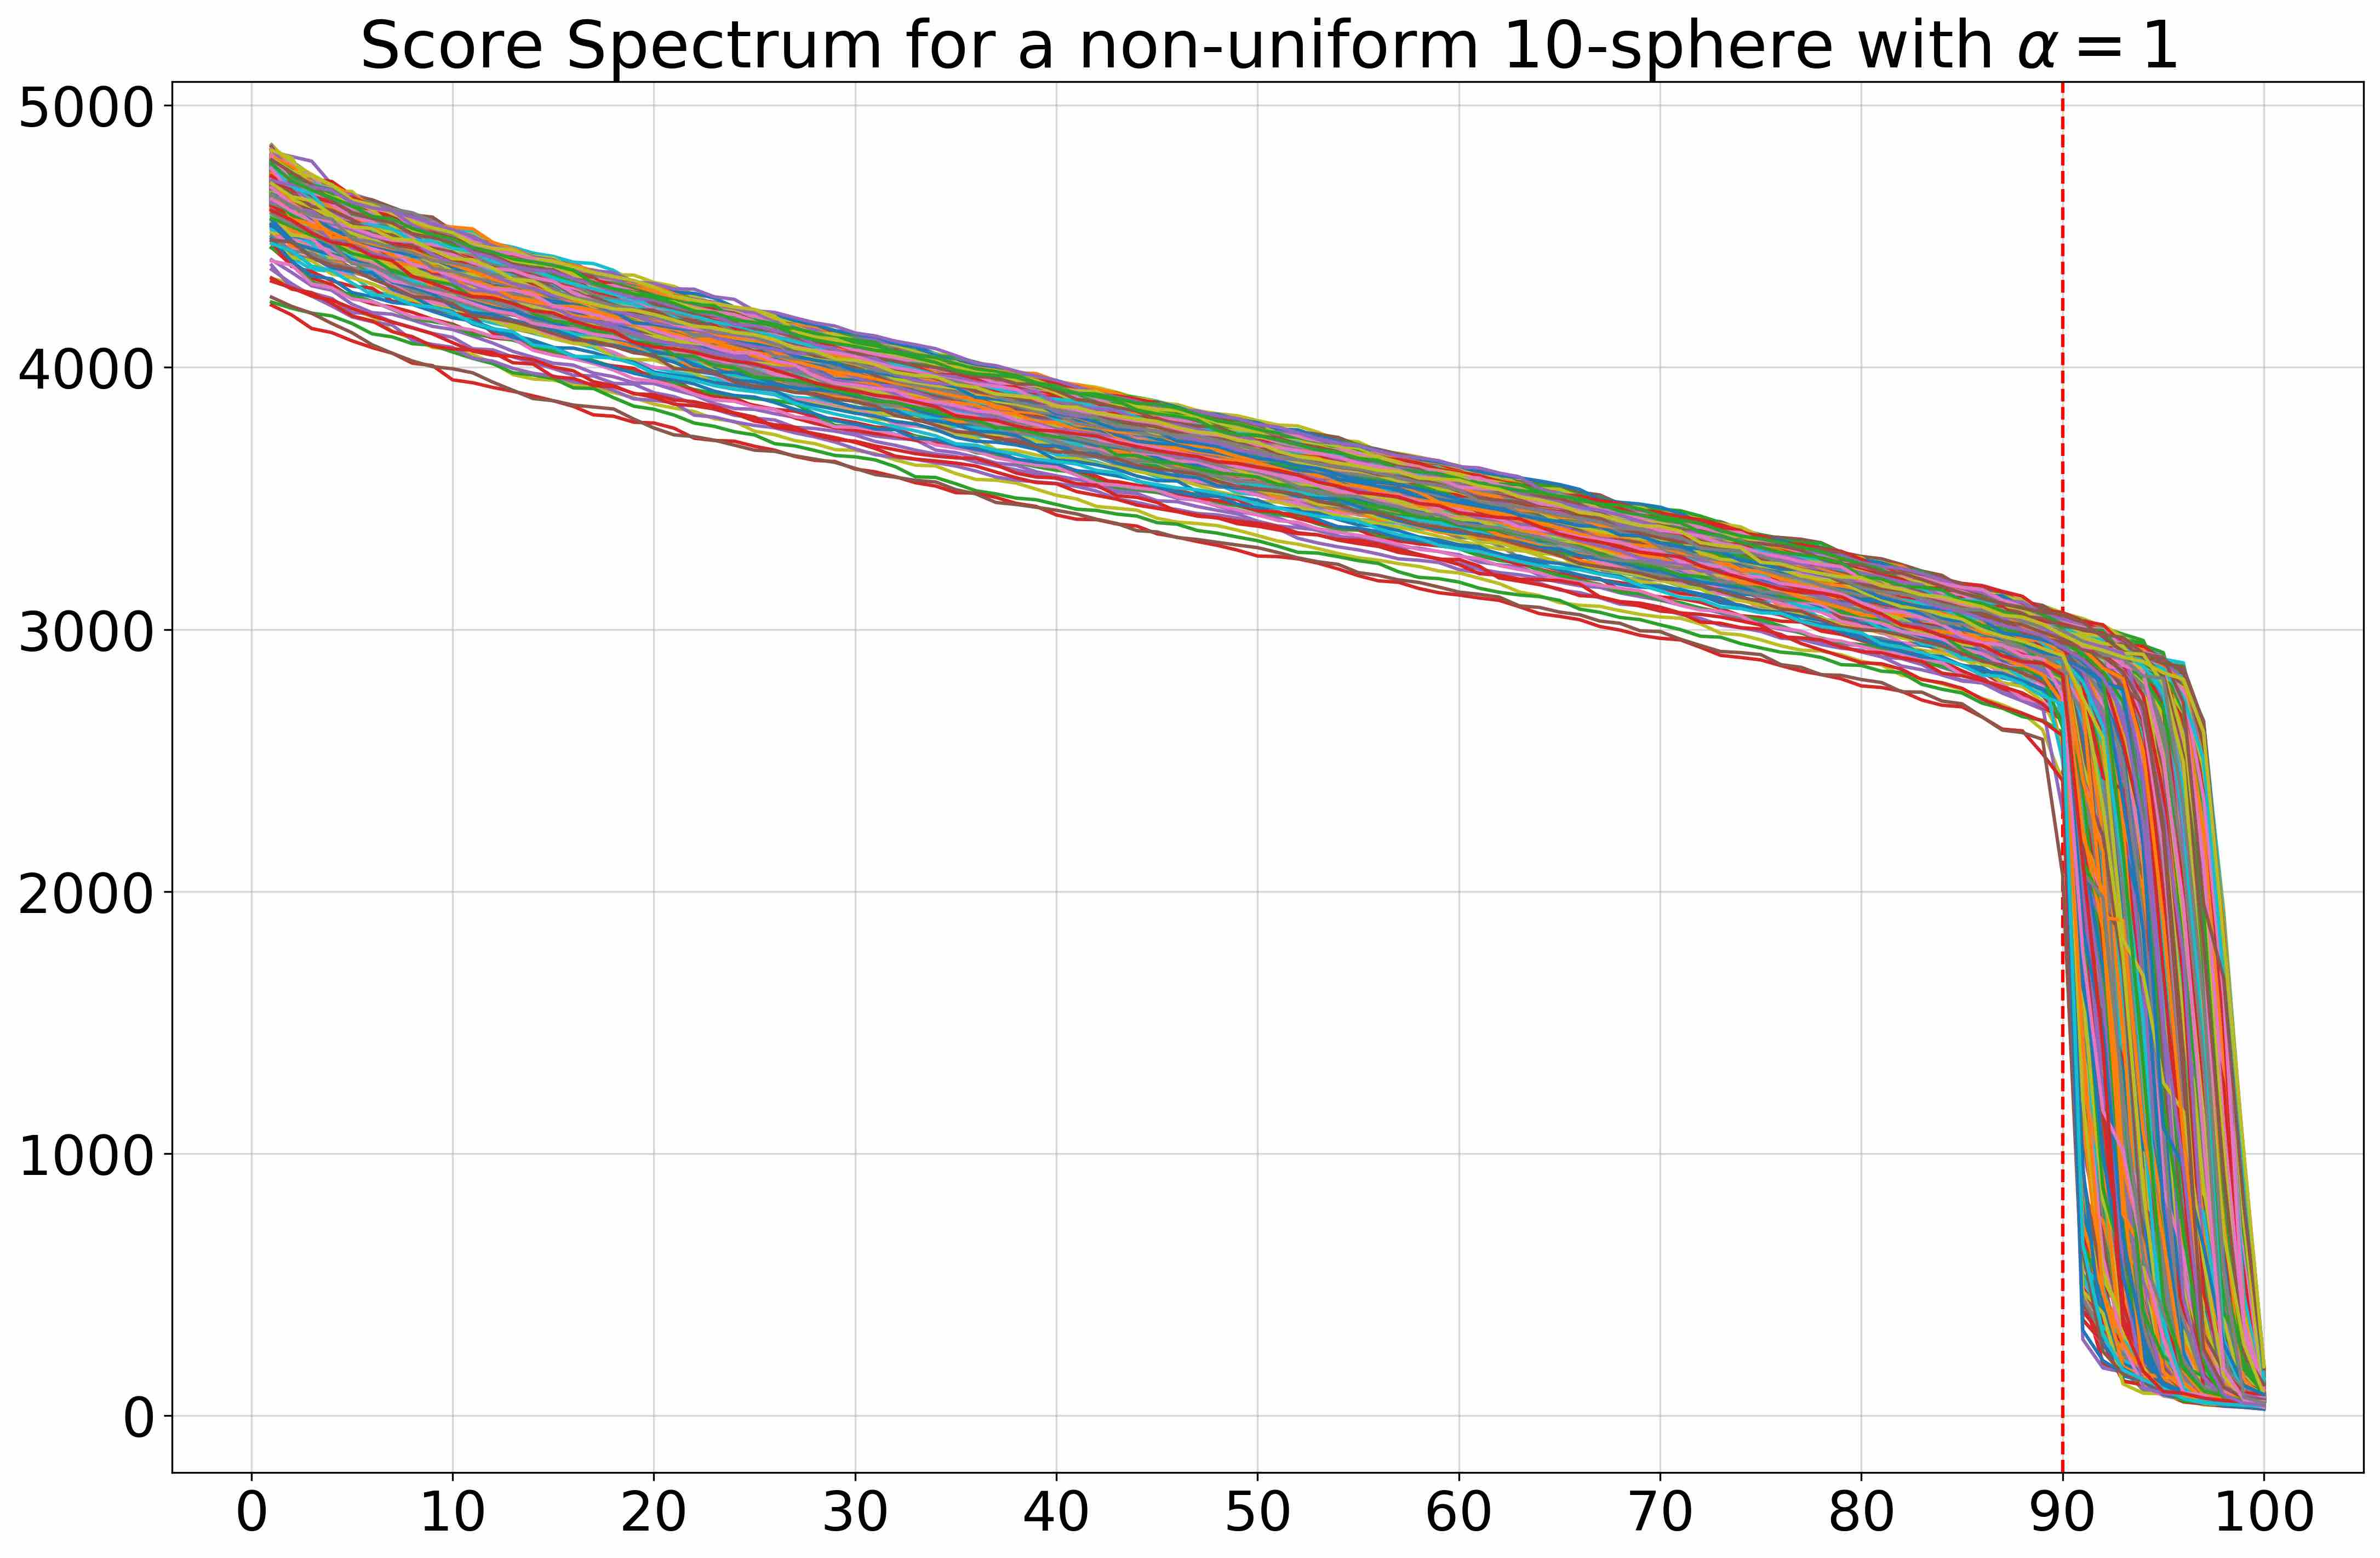
\includegraphics[width=0.95\linewidth]{chapter3/figures/non_uniform/spectrum_1.jpg}
        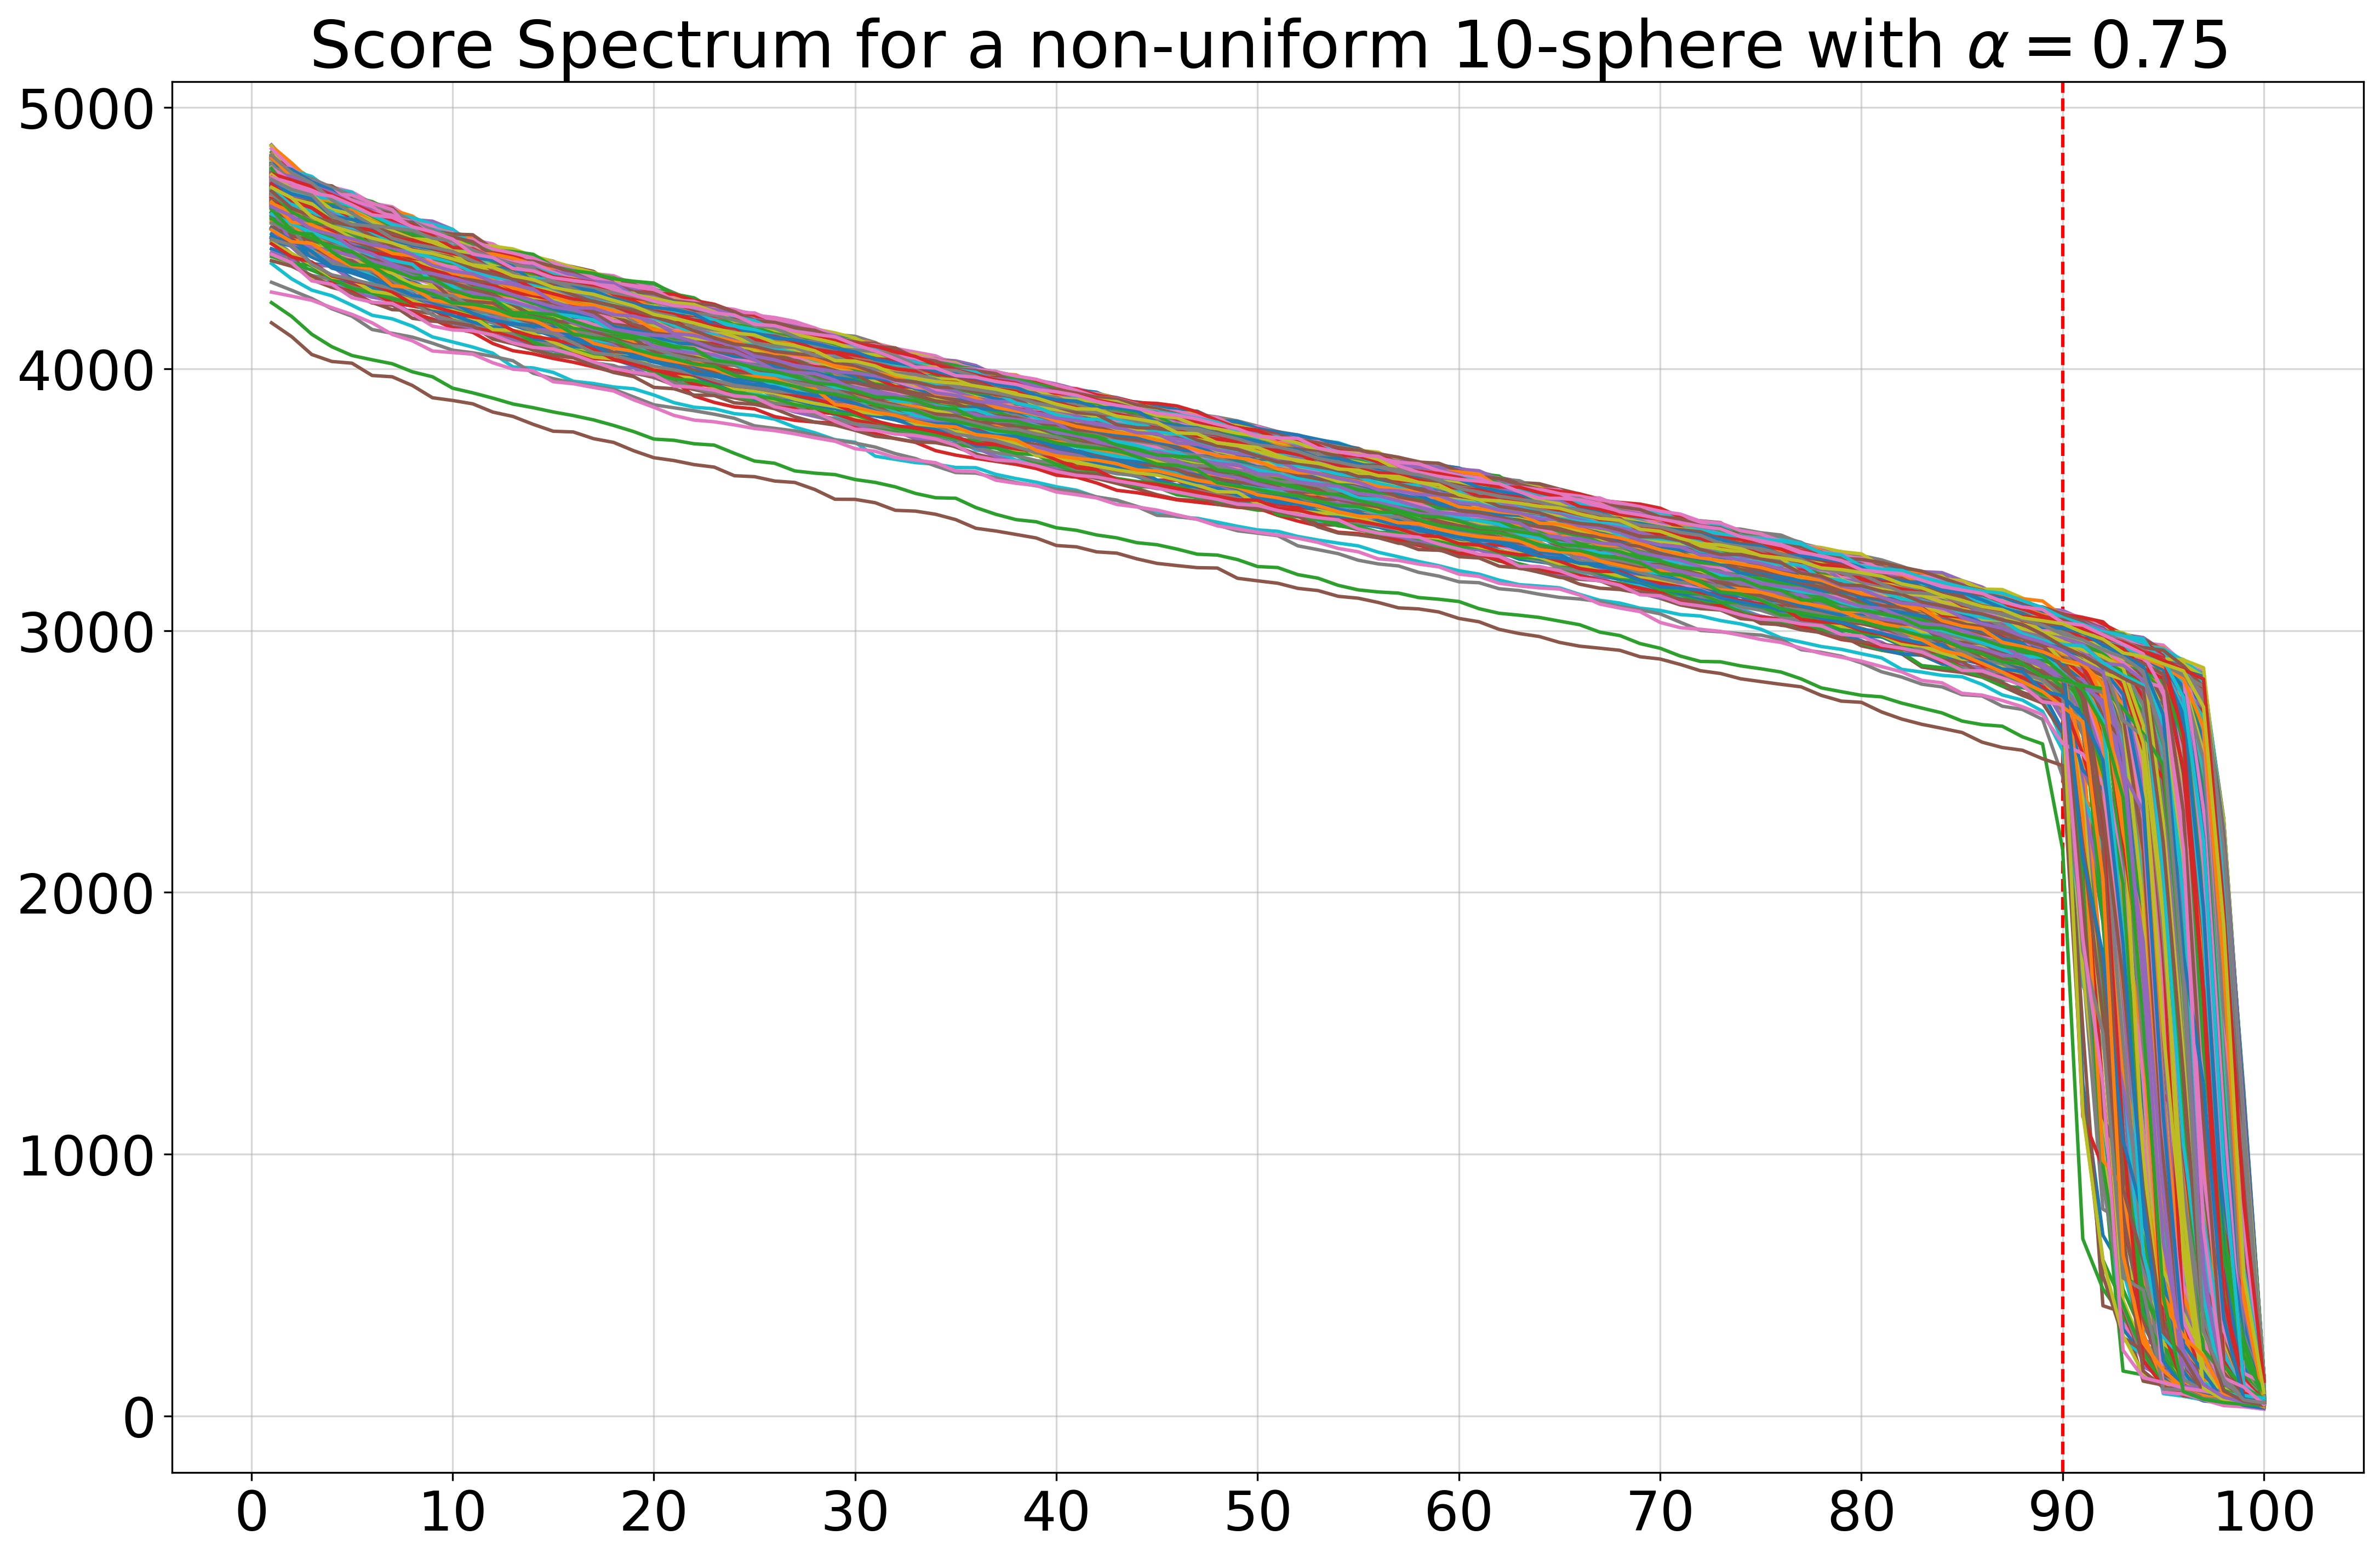
\includegraphics[width=0.95\linewidth]{chapter3/figures/non_uniform/spectrum_0.75.jpg}
        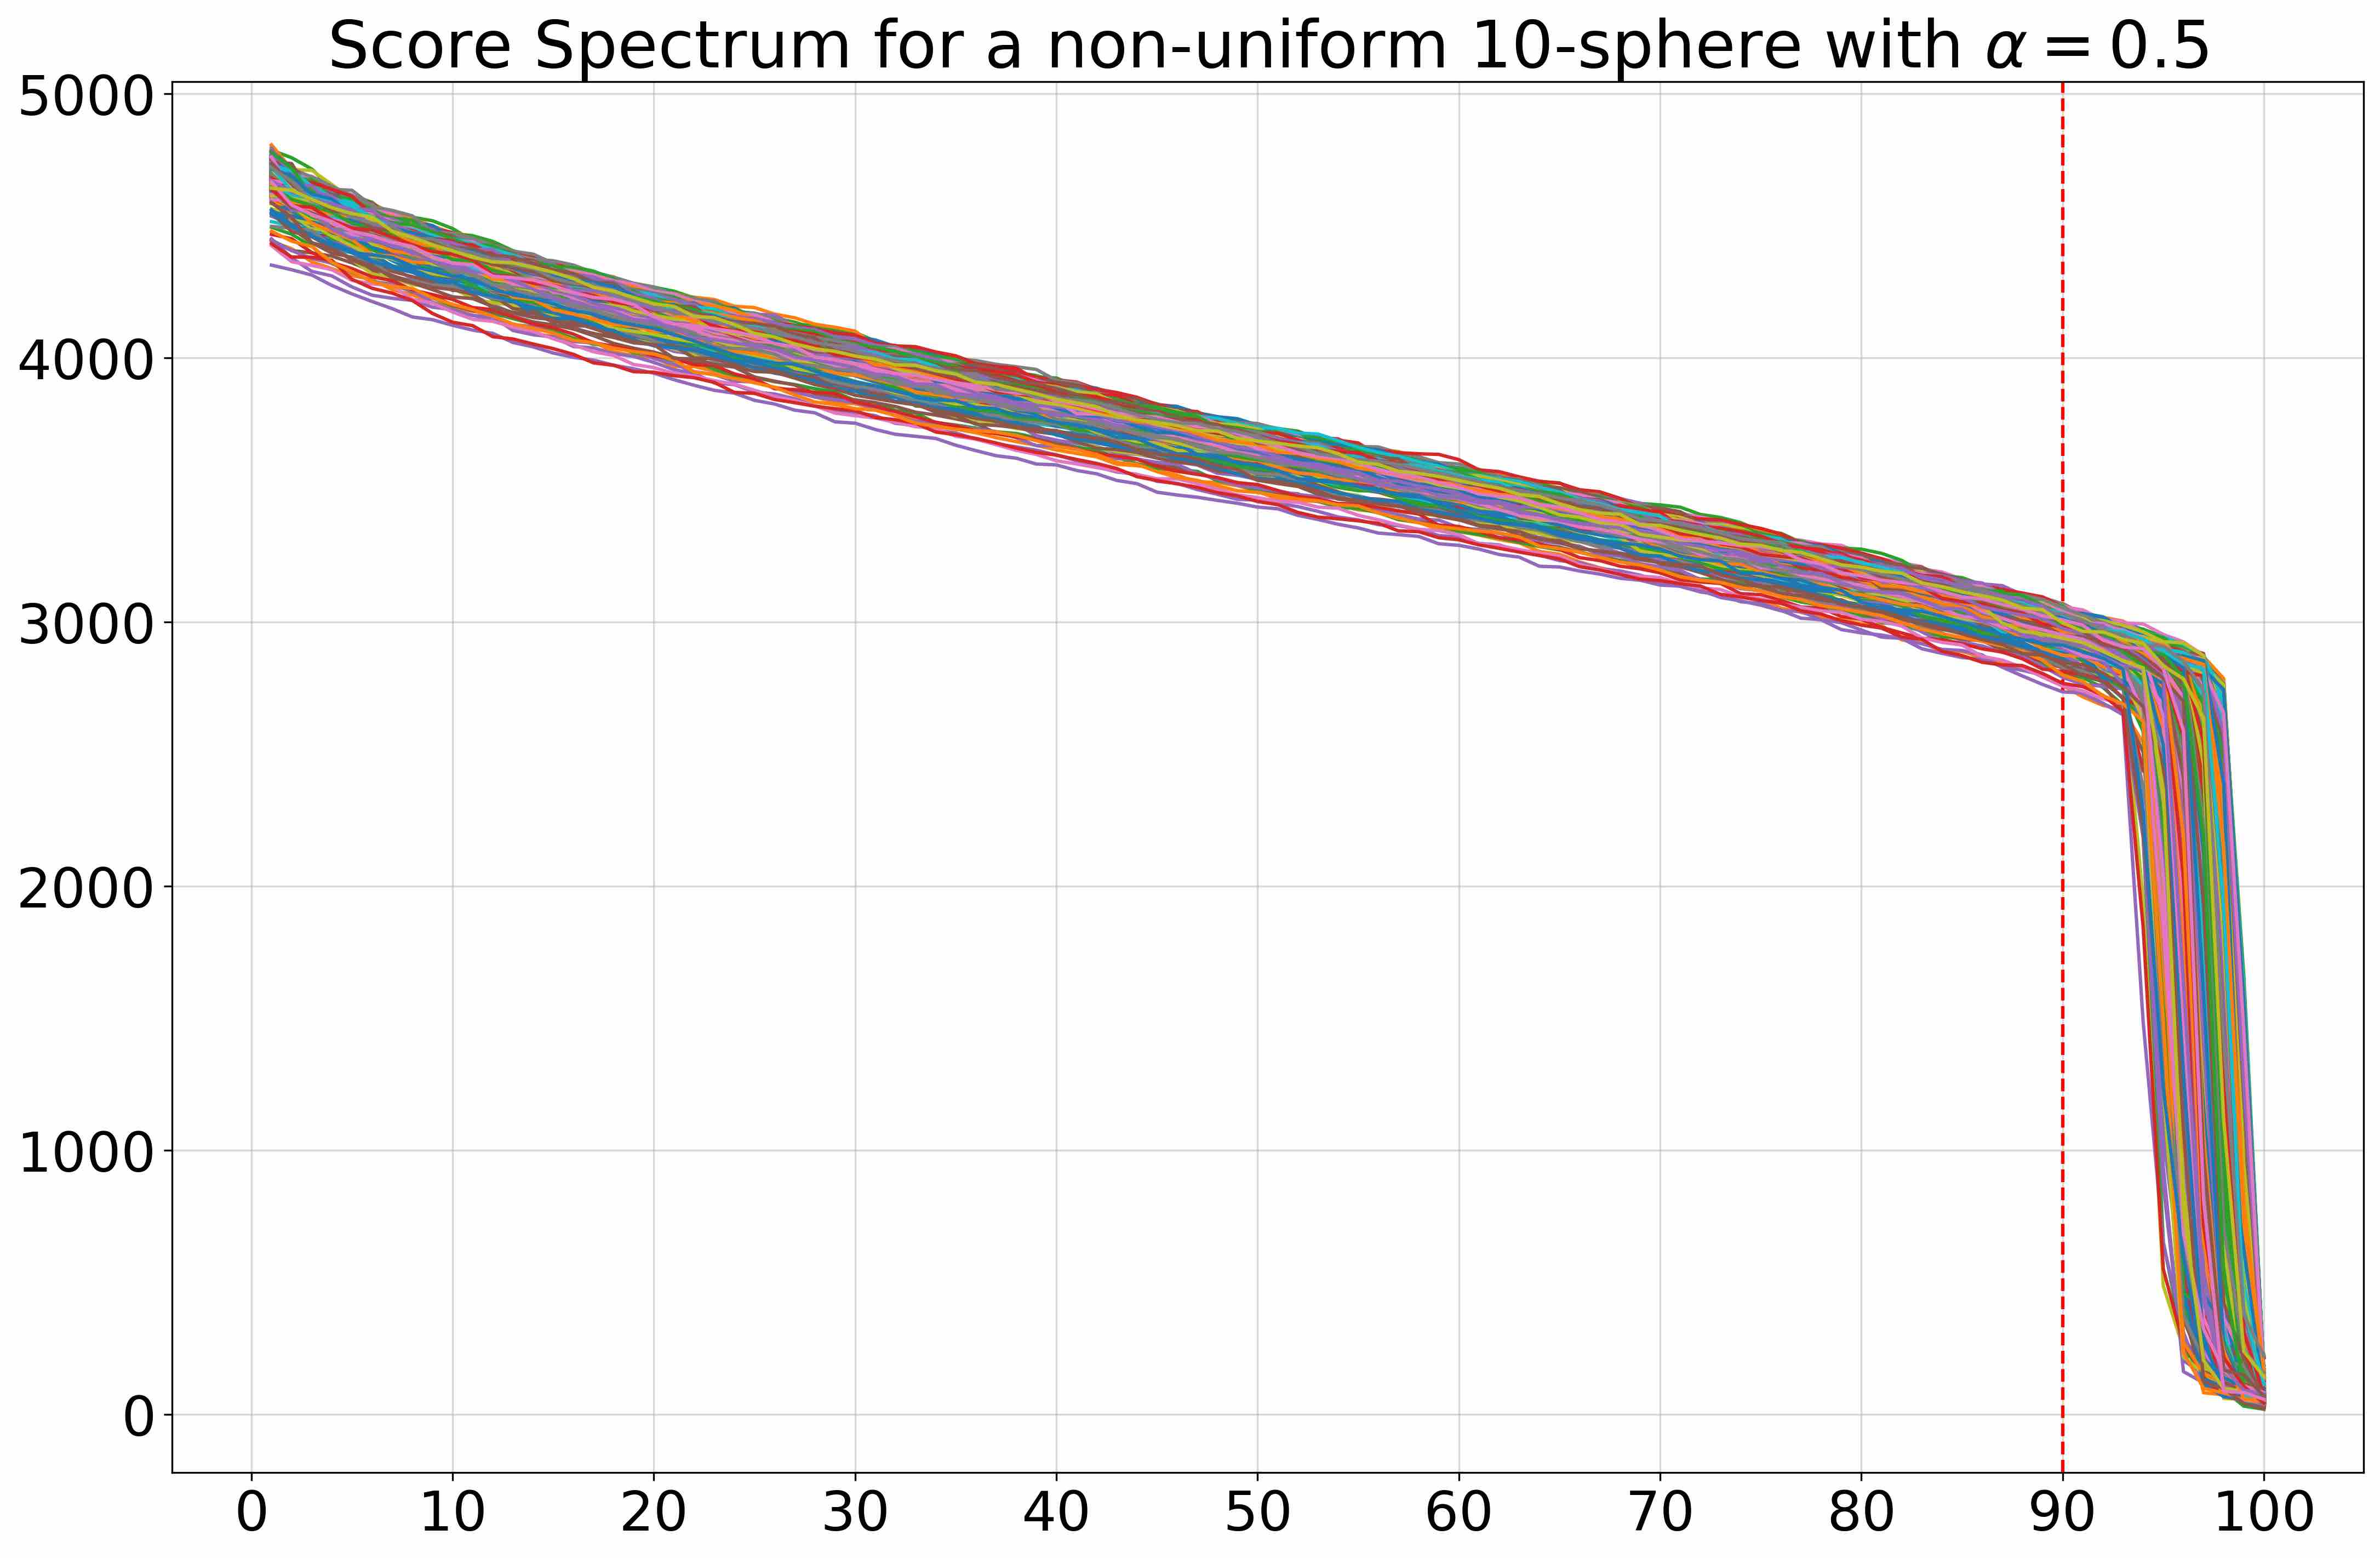
\includegraphics[width=0.95\linewidth]{chapter3/figures/non_uniform/spectrum_0.5.jpg}
    \end{minipage}
    \begin{minipage}[t]{0.5\textwidth}
        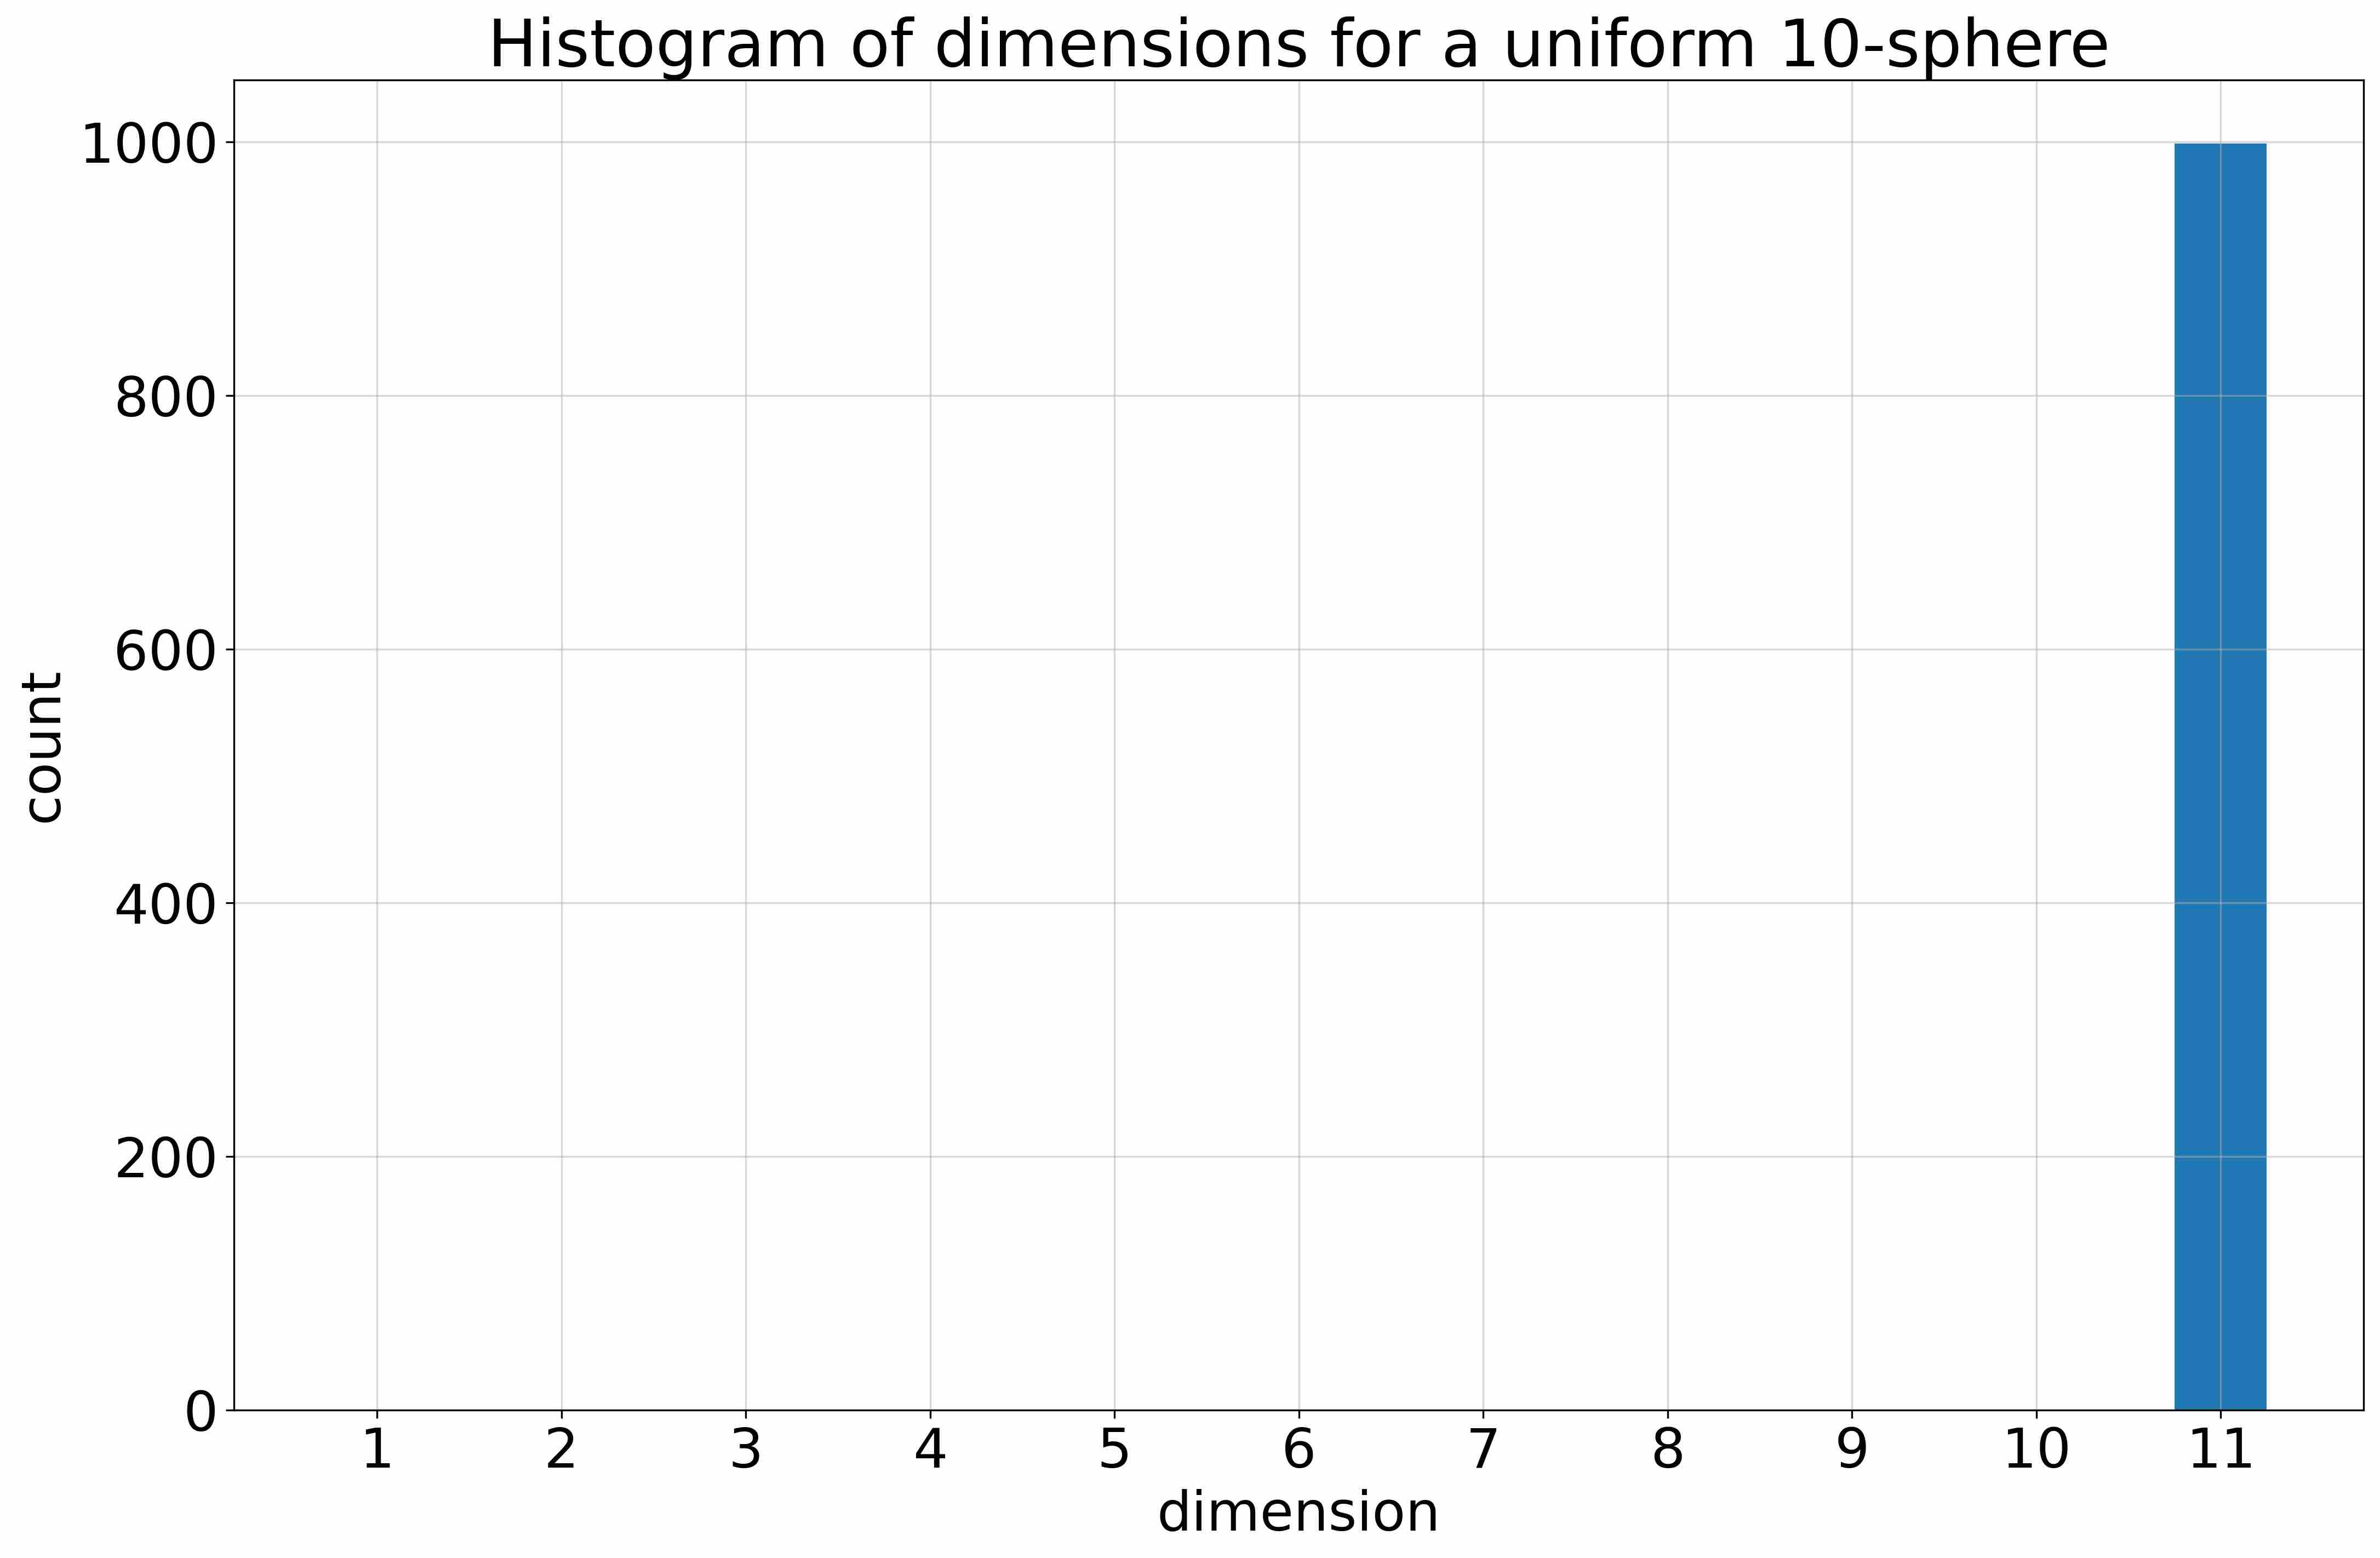
\includegraphics[width=0.95\linewidth]{chapter3/figures/non_uniform/dims_0.jpg}
        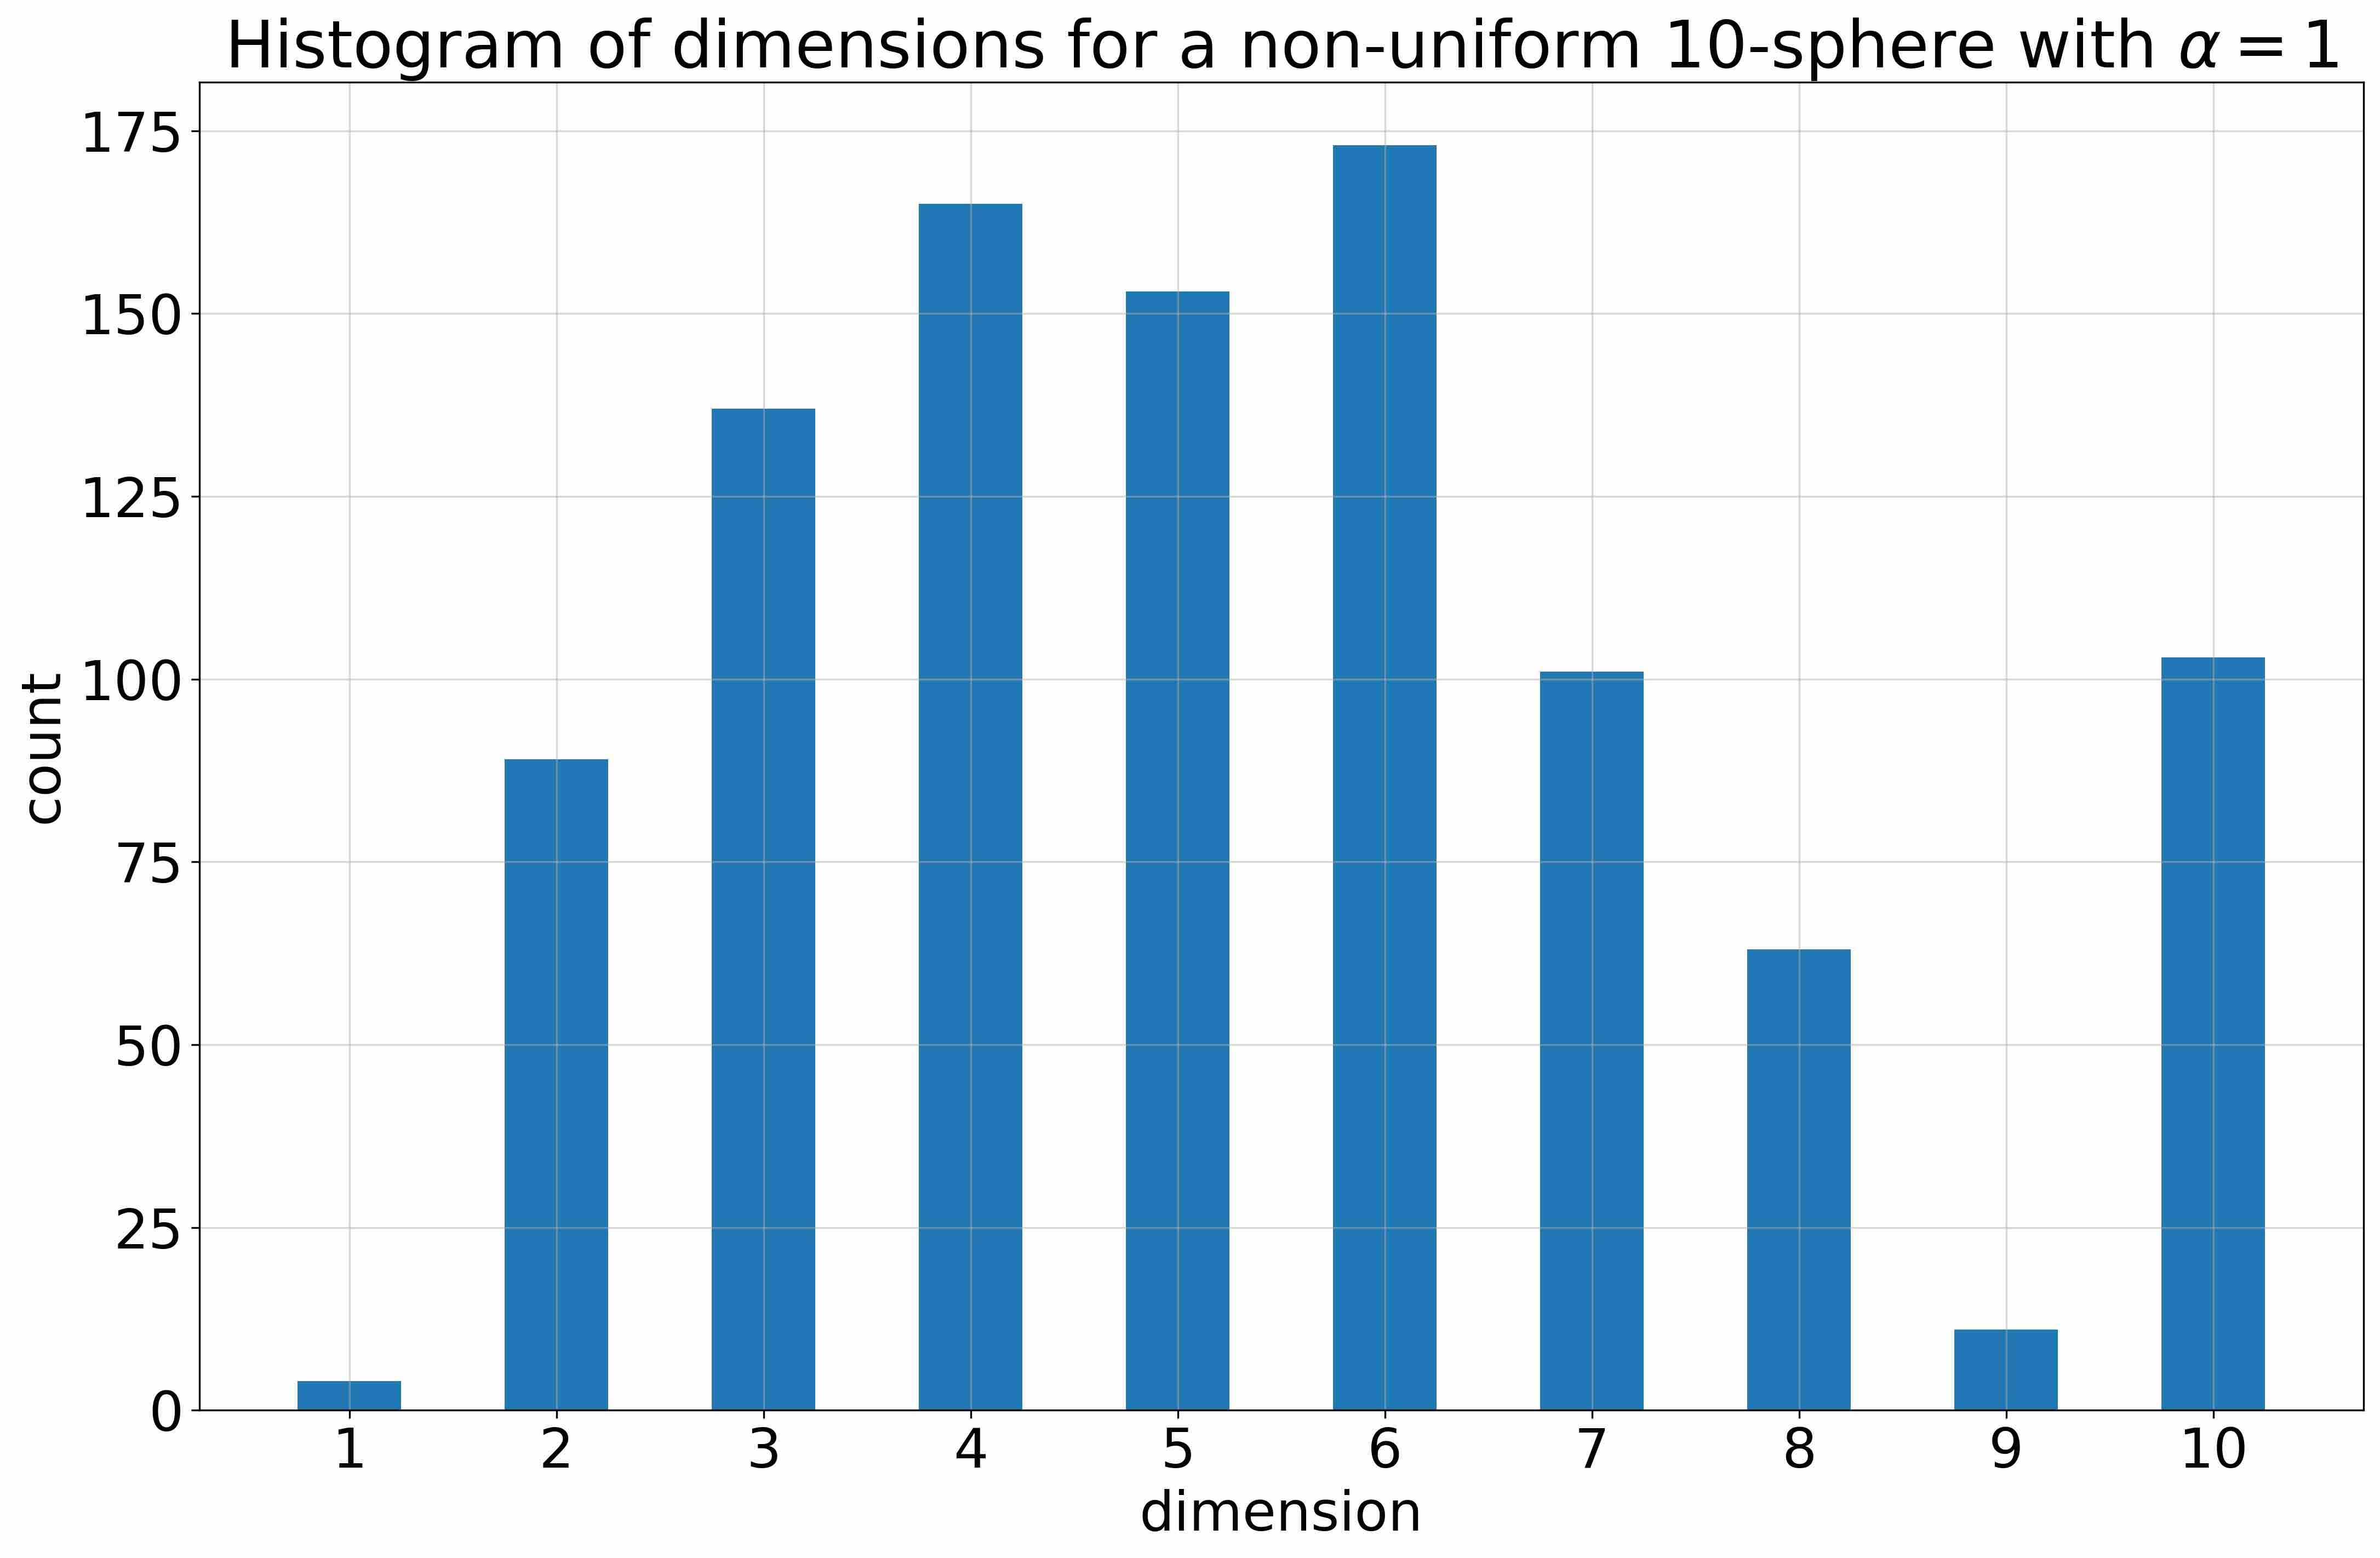
\includegraphics[width=0.95\linewidth]{chapter3/figures/non_uniform/dims_1.jpg}
        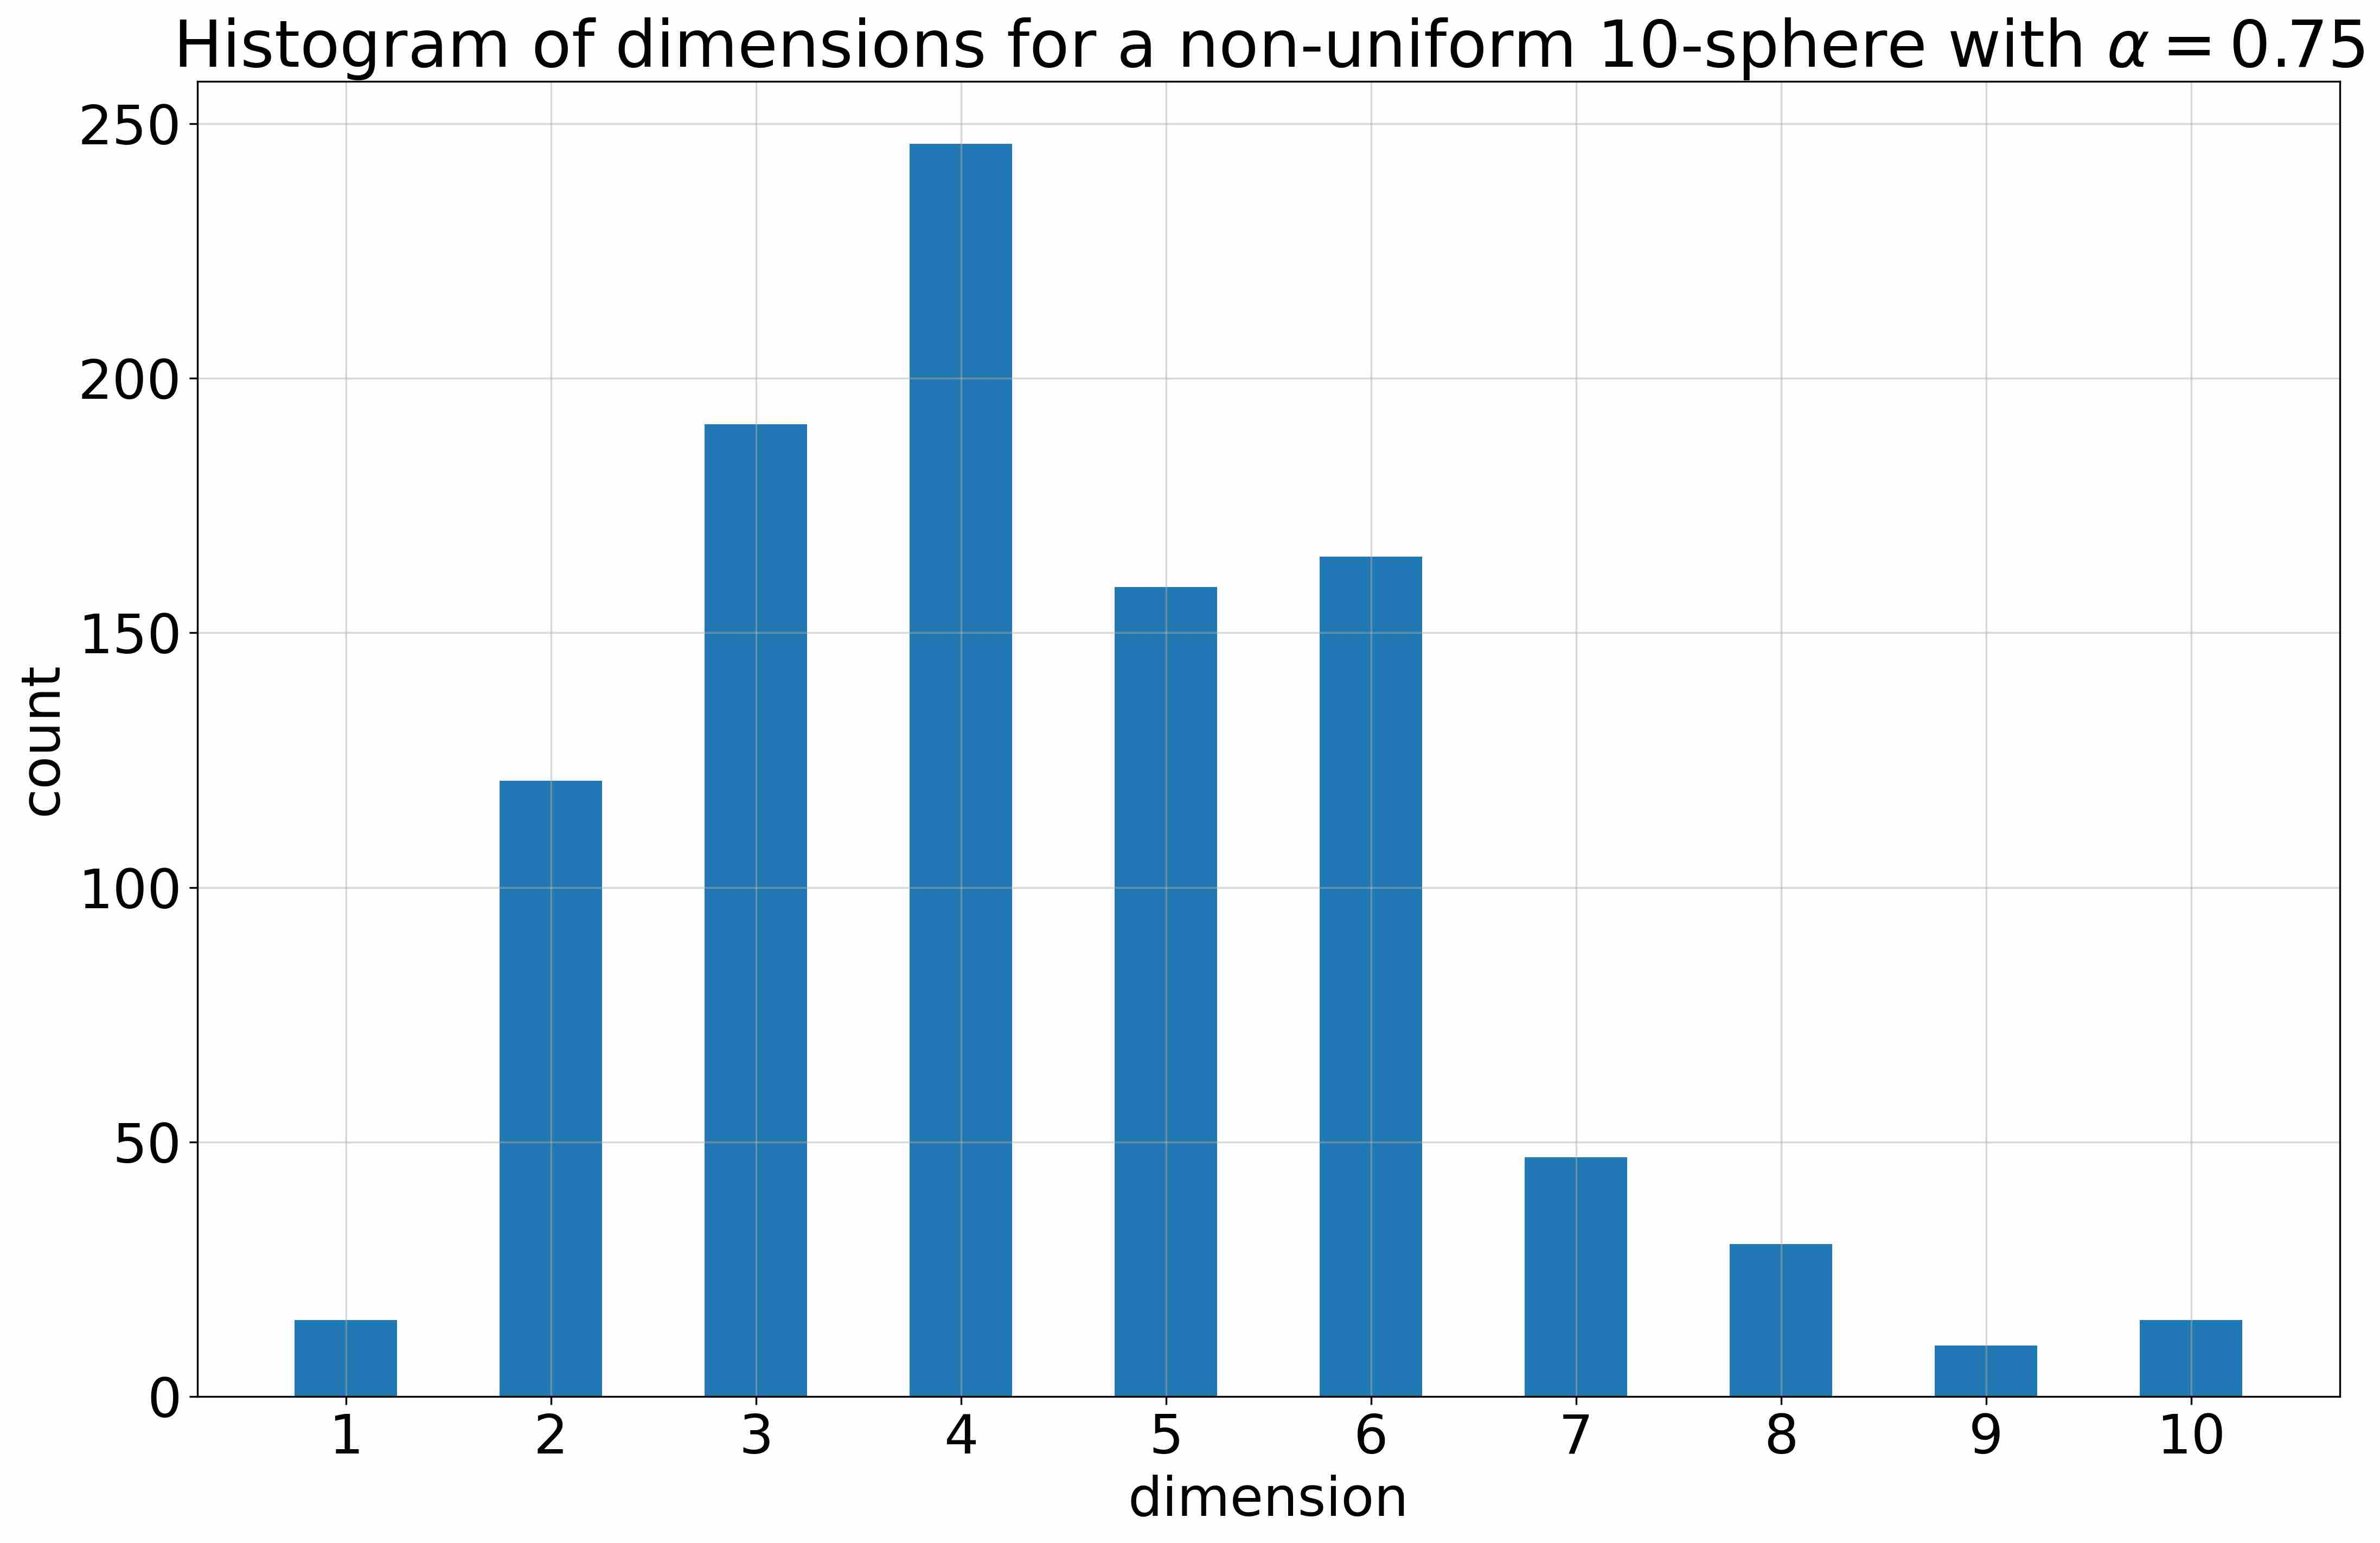
\includegraphics[width=0.95\linewidth]{chapter3/figures/non_uniform/dims_0.75.jpg}
        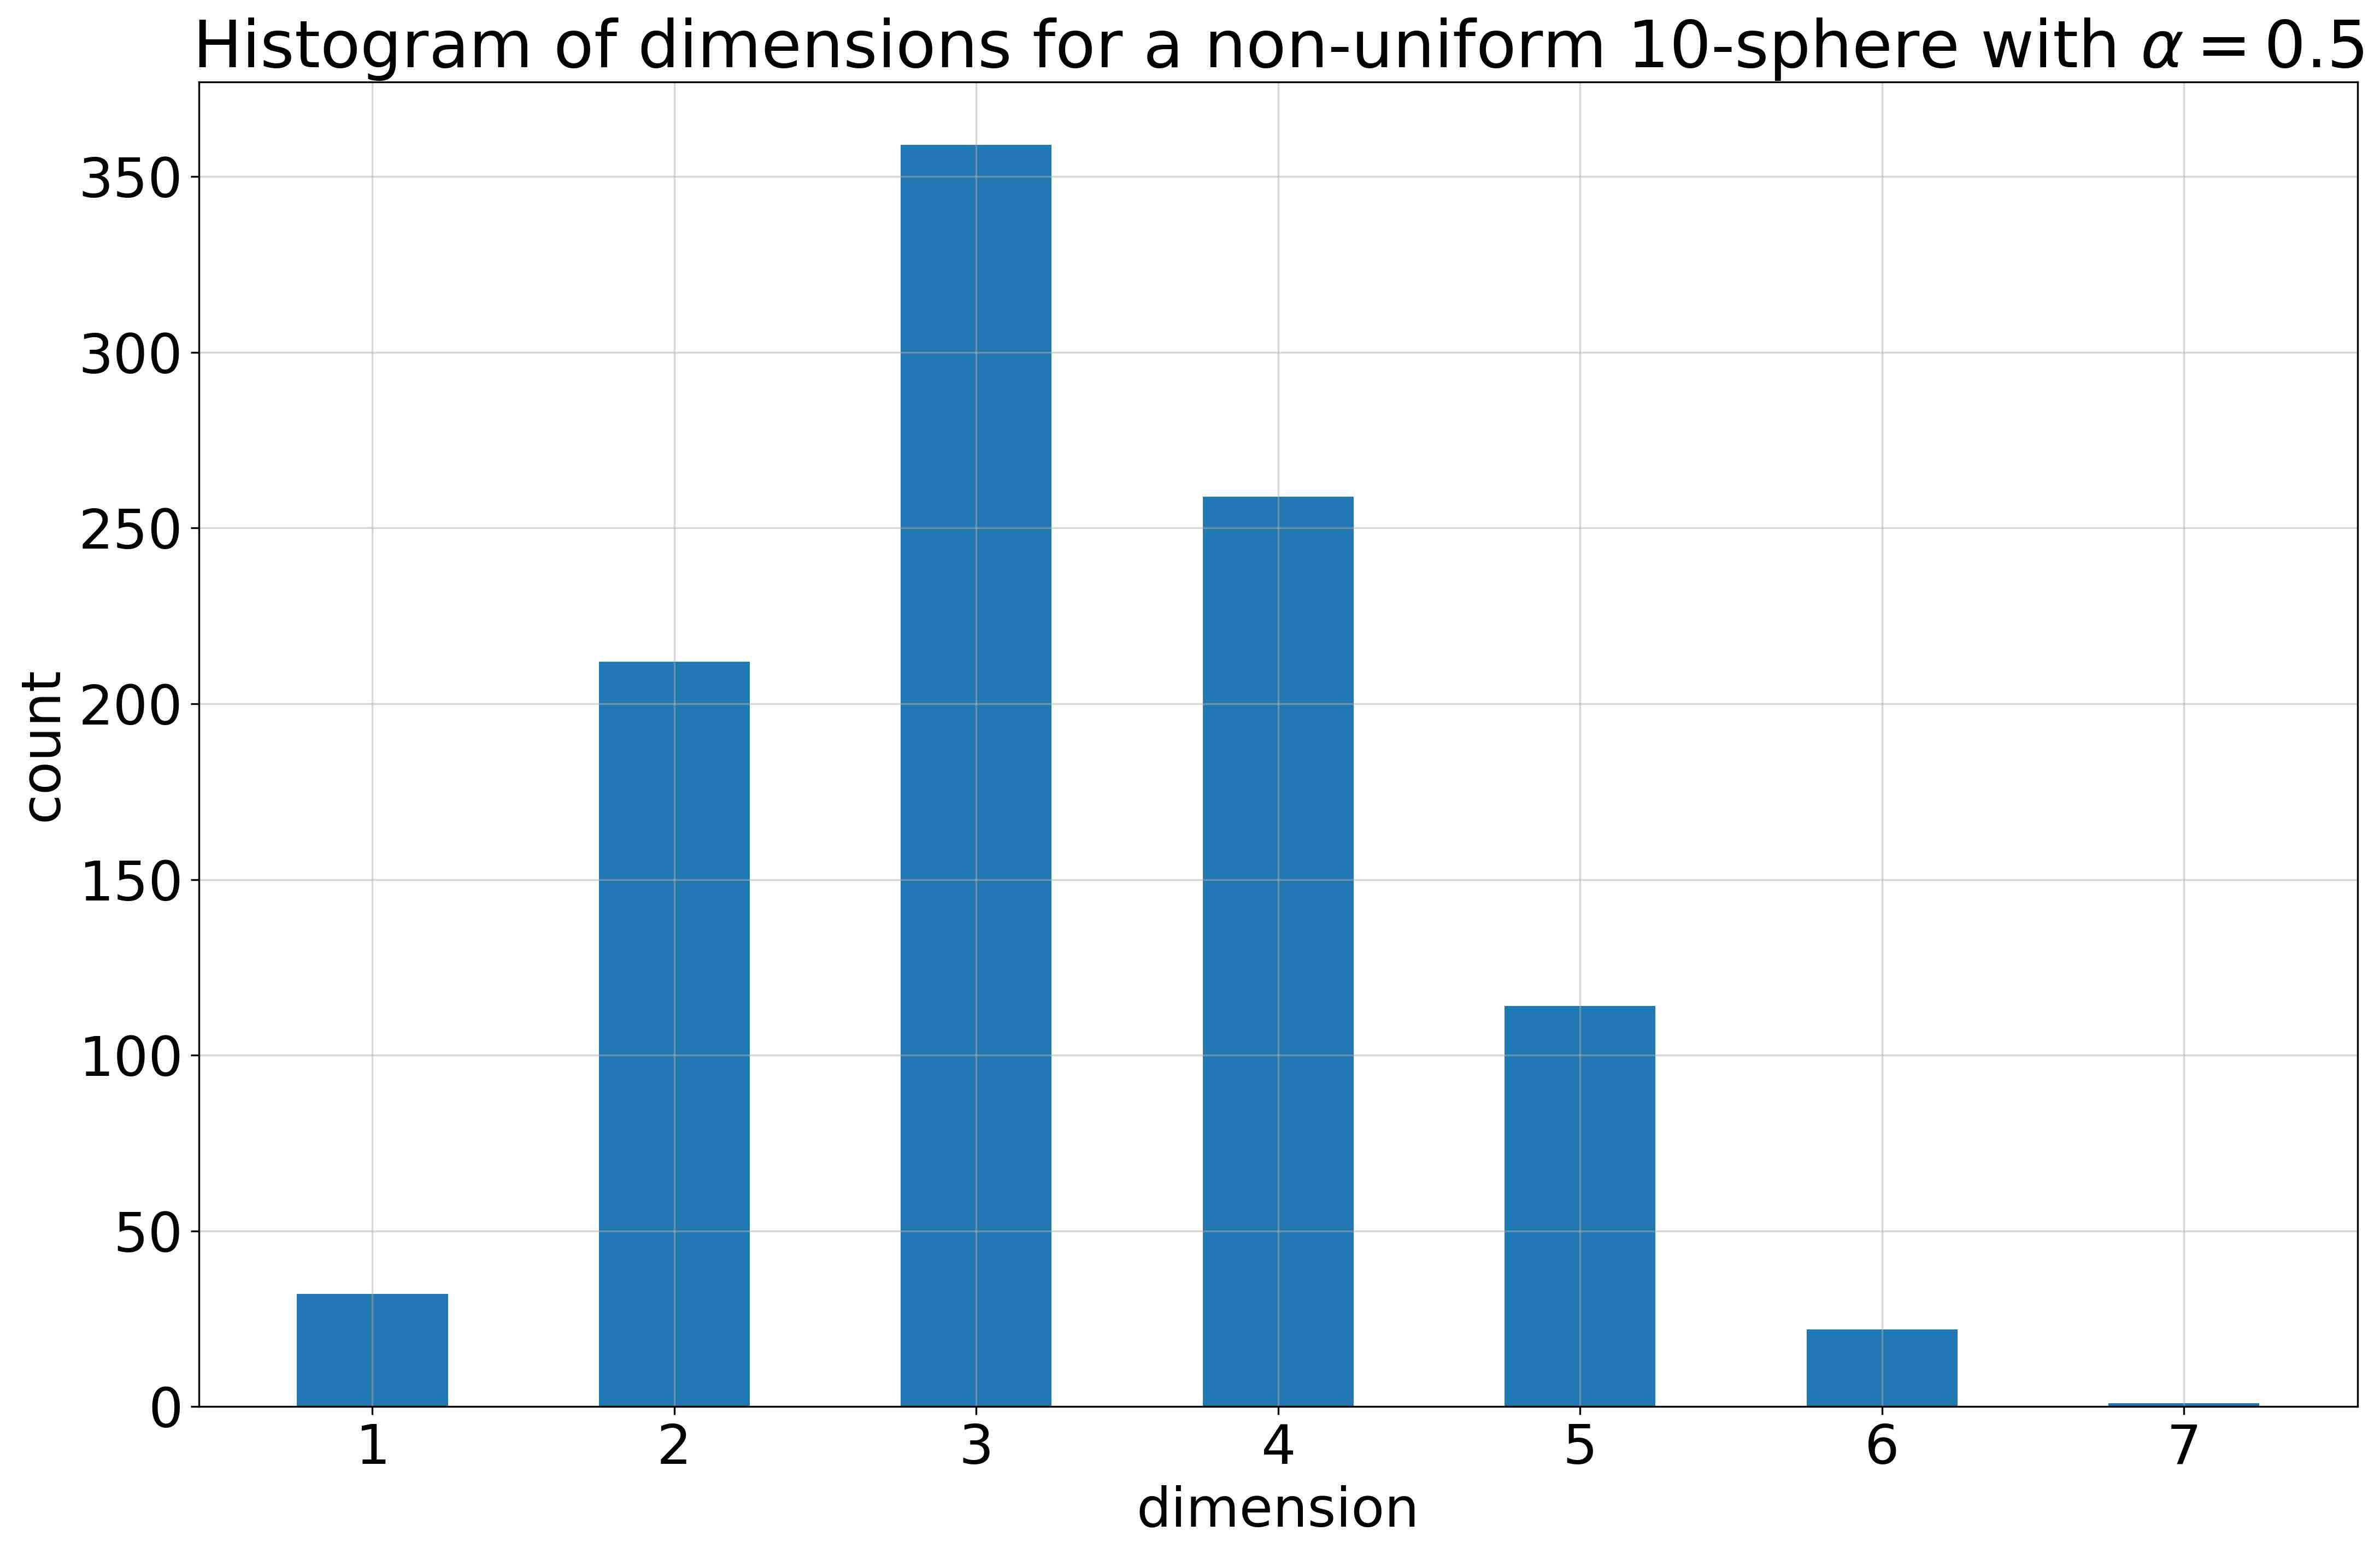
\includegraphics[width=0.95\linewidth]{chapter3/figures/non_uniform/dims_0.5.jpg}
    \end{minipage}
    \caption{Dimensionality estimates for uniform and non-uniform distributions on a 10-sphere. On the right, we present histograms showing how many points $\textbf{x}_0^{(j)}$ result in a given $\hat{k}(\textbf{x}_0^{(j)})$. Taking $\hat{k} = \max_j \hat{k}(\textbf{x}_0^{(j)})$ allows for robust estimation for moderate values of the concentration parameter $\alpha$.}
    \label{ch3:fig:non_uniform}
\end{figure*}

    
    \subsection{Relaxing the strict manifold assumption}
    The proof of the Theorem \ref{ch3:thm:score_orthogonal} assumes that $p_0$ is strictly contained on the data manifold $\mathcal{M}$, however in practice it is possible that the data distribution is concentrated around $\mathcal{M}$ rather then being contained within. Therefore, we conduct an empirical analysis, which examines how our method works in the case of the data contained around the manifold. We start with $p_0$ a uniform distribution on a unit $25$-sphere embedded in a 100 dimensional space and convolve it with a Gaussian distribution $\mathcal{N}(0, \sigma \mathbf{I})$ to obtain a distribution $p_0^\sigma$ that concentrates around $\mathcal{M}$. As $\sigma$ increases the distribution is blurred out more and more into the ambient space. We train score model on each of the resulting distributions and use our method to estimate the dimension. We find that our method produces correct estimation for for small values of $\sigma$ i.e. when $p_0^\sigma$ is still concentrated tightly around $\mathcal{M}$. This is expected since of high values of $\sigma$ the distribution isn't really concentrated around any manifold and therefore the notion of intrinsic dimension doesn't make any sense. The results are presented in Figure \ref{ch3:fig:robustness_samples}.
    
    \begin{figure}
        \centering
        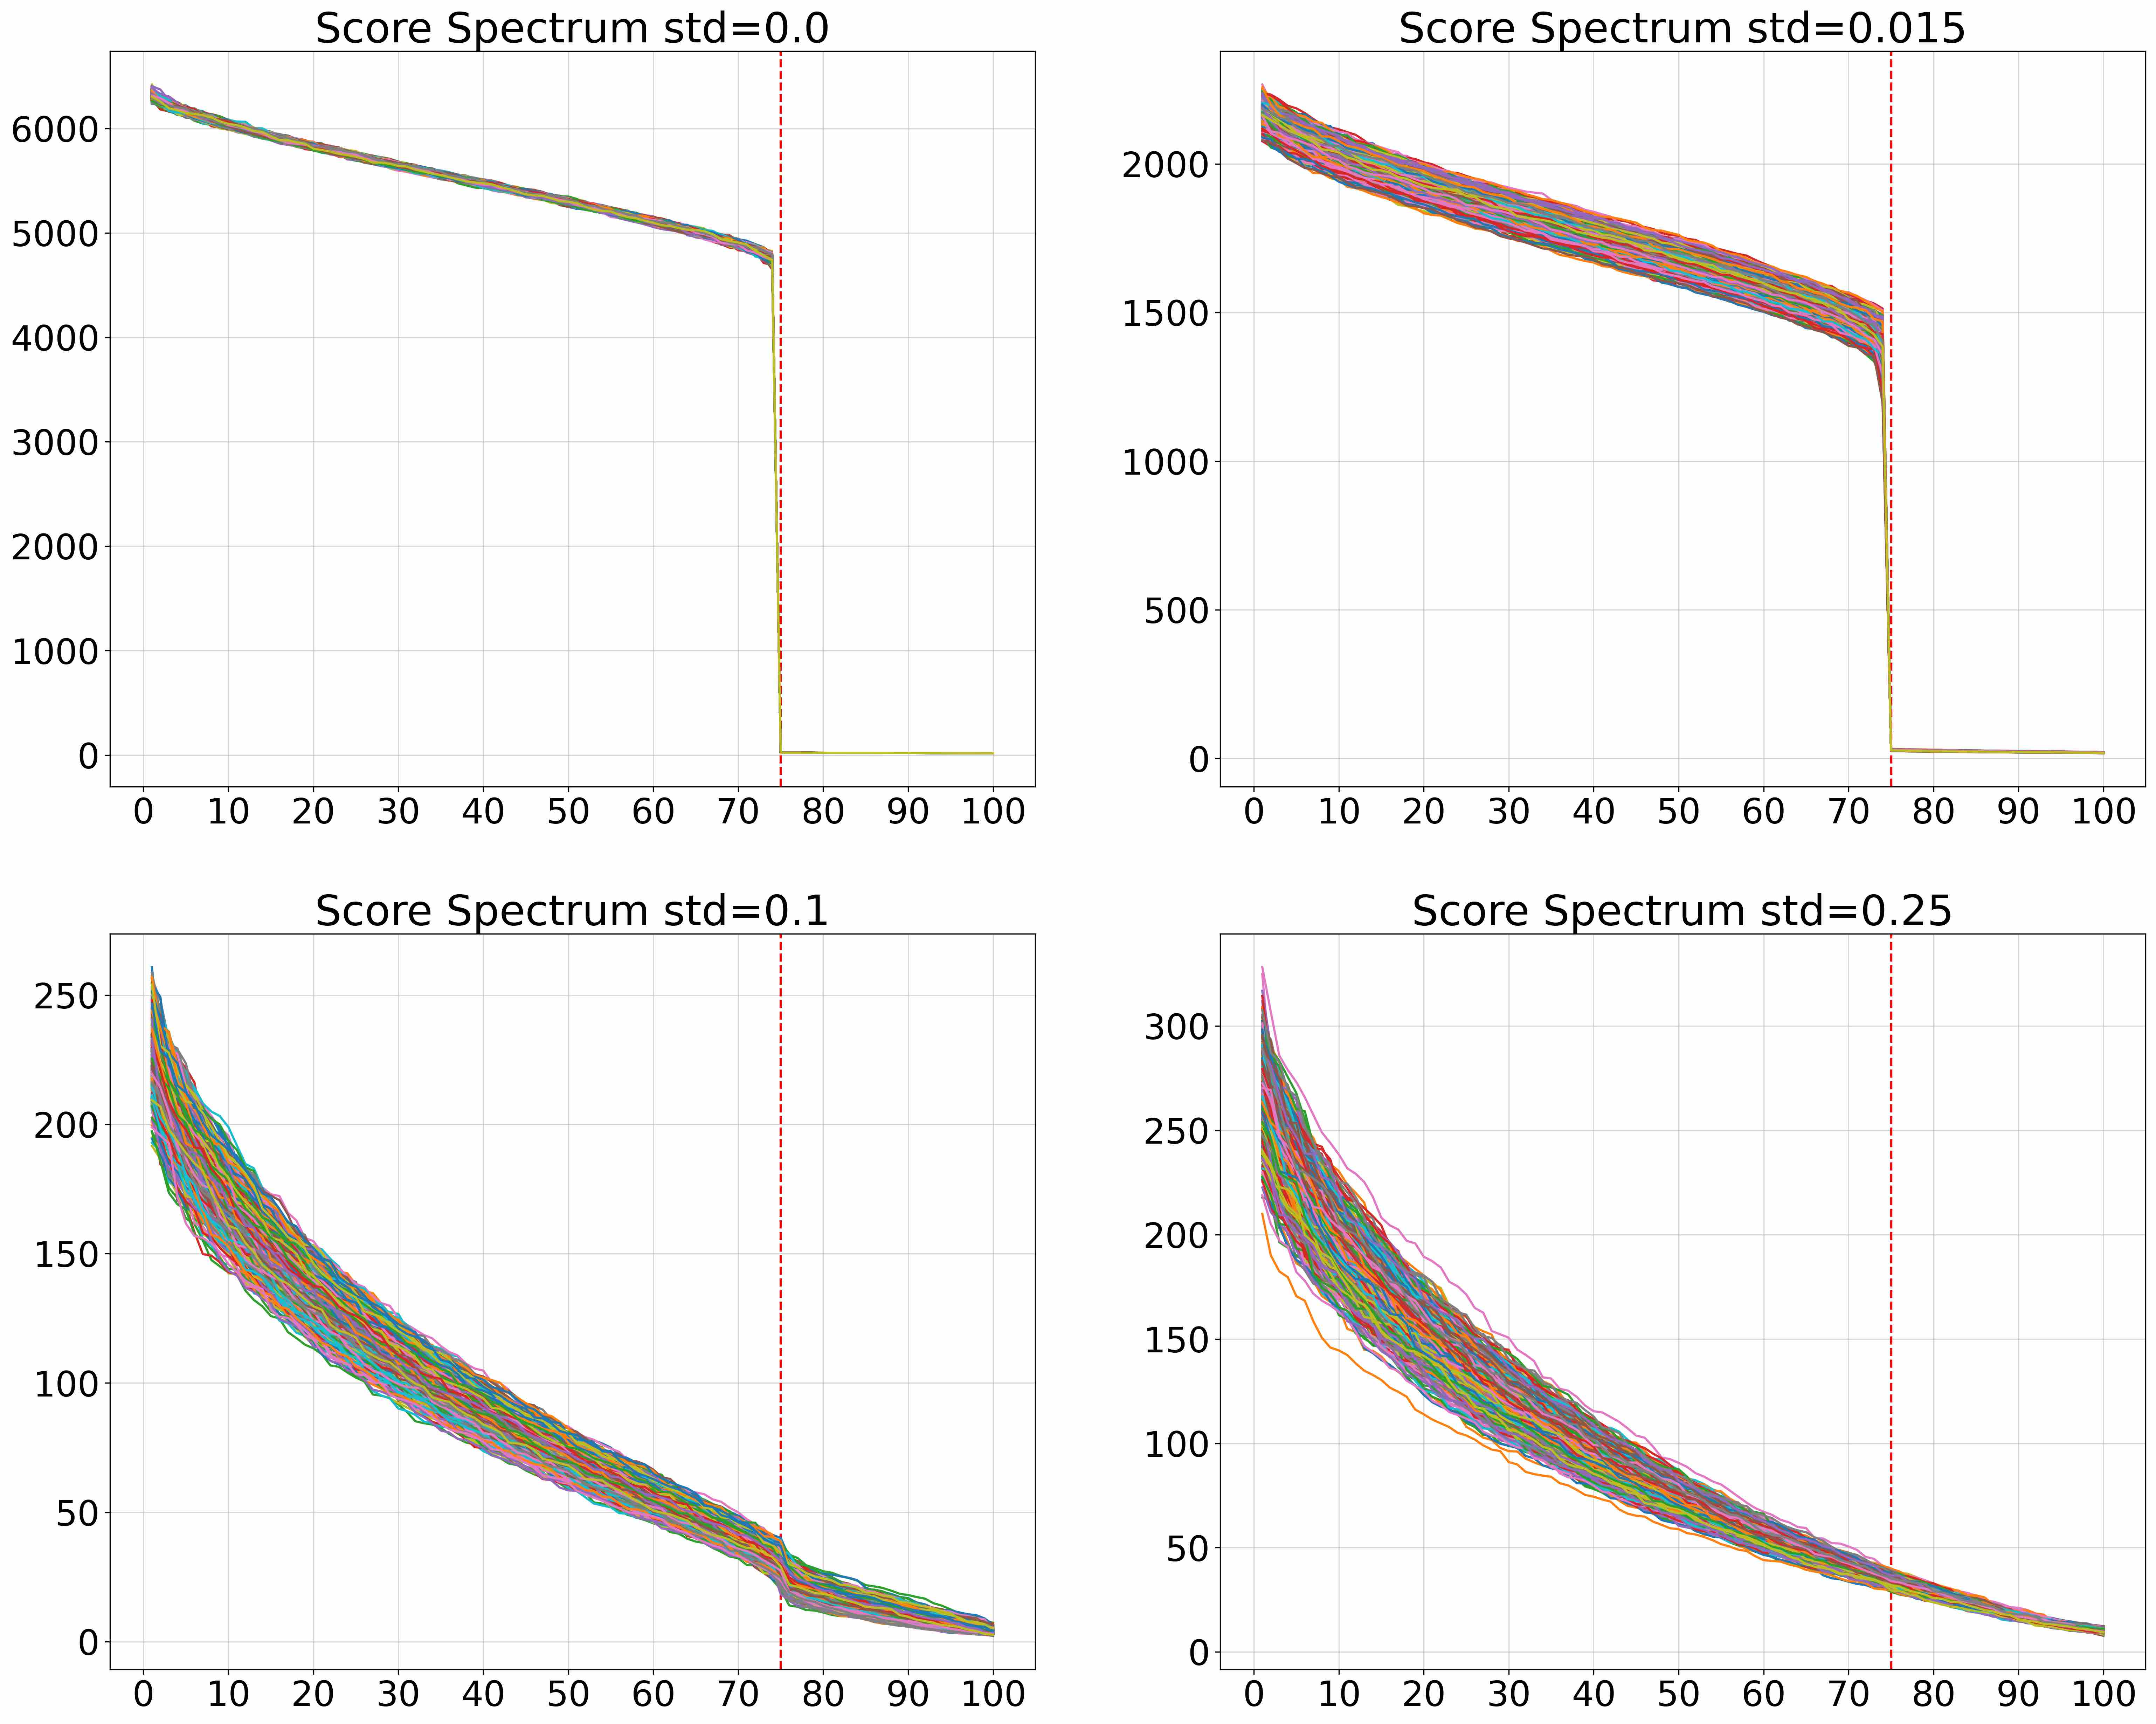
\includegraphics[width=\textwidth]{chapter3/figures/robustness_samples.jpg}
        \caption{Score spectra for score models on 25-sphere trained on noisy manifold data.}
        \label{ch3:fig:robustness_samples}
    \end{figure}

    
